\documentclass[twoside]{book}

% Packages required by doxygen
\usepackage{calc}
\usepackage{doxygen}
\usepackage{graphicx}
\usepackage[utf8]{inputenc}
\usepackage{makeidx}
\usepackage{multicol}
\usepackage{multirow}
\usepackage{textcomp}
\usepackage[table]{xcolor}

% Font selection
\usepackage[T1]{fontenc}
\usepackage{mathptmx}
\usepackage[scaled=.90]{helvet}
\usepackage{courier}
\usepackage{amssymb}
\usepackage{sectsty}
\renewcommand{\familydefault}{\sfdefault}
\allsectionsfont{%
  \fontseries{bc}\selectfont%
  \color{darkgray}%
}
\renewcommand{\DoxyLabelFont}{%
  \fontseries{bc}\selectfont%
  \color{darkgray}%
}

% Page & text layout
\usepackage{geometry}
\geometry{%
  a4paper,%
  top=2.5cm,%
  bottom=2.5cm,%
  left=2.5cm,%
  right=2.5cm%
}
\tolerance=750
\hfuzz=15pt
\hbadness=750
\setlength{\emergencystretch}{15pt}
\setlength{\parindent}{0cm}
\setlength{\parskip}{0.2cm}
\makeatletter
\renewcommand{\paragraph}{%
  \@startsection{paragraph}{4}{0ex}{-1.0ex}{1.0ex}{%
    \normalfont\normalsize\bfseries\SS@parafont%
  }%
}
\renewcommand{\subparagraph}{%
  \@startsection{subparagraph}{5}{0ex}{-1.0ex}{1.0ex}{%
    \normalfont\normalsize\bfseries\SS@subparafont%
  }%
}
\makeatother

% Headers & footers
\usepackage{fancyhdr}
\pagestyle{fancyplain}
\fancyhead[LE]{\fancyplain{}{\bfseries\thepage}}
\fancyhead[CE]{\fancyplain{}{}}
\fancyhead[RE]{\fancyplain{}{\bfseries\leftmark}}
\fancyhead[LO]{\fancyplain{}{\bfseries\rightmark}}
\fancyhead[CO]{\fancyplain{}{}}
\fancyhead[RO]{\fancyplain{}{\bfseries\thepage}}
\fancyfoot[LE]{\fancyplain{}{}}
\fancyfoot[CE]{\fancyplain{}{}}
\fancyfoot[RE]{\fancyplain{}{\bfseries\scriptsize Generated on Fri Apr 18 2014 23\-:45\-:46 for I\-S\-E by Doxygen }}
\fancyfoot[LO]{\fancyplain{}{\bfseries\scriptsize Generated on Fri Apr 18 2014 23\-:45\-:46 for I\-S\-E by Doxygen }}
\fancyfoot[CO]{\fancyplain{}{}}
\fancyfoot[RO]{\fancyplain{}{}}
\renewcommand{\footrulewidth}{0.4pt}
\renewcommand{\chaptermark}[1]{%
  \markboth{#1}{}%
}
\renewcommand{\sectionmark}[1]{%
  \markright{\thesection\ #1}%
}

% Indices & bibliography
\usepackage{natbib}
\usepackage[titles]{tocloft}
\setcounter{tocdepth}{3}
\setcounter{secnumdepth}{5}
\makeindex

% Hyperlinks (required, but should be loaded last)
\usepackage{ifpdf}
\ifpdf
  \usepackage[pdftex,pagebackref=true]{hyperref}
\else
  \usepackage[ps2pdf,pagebackref=true]{hyperref}
\fi
\hypersetup{%
  colorlinks=true,%
  linkcolor=blue,%
  citecolor=blue,%
  unicode%
}

% Custom commands
\newcommand{\clearemptydoublepage}{%
  \newpage{\pagestyle{empty}\cleardoublepage}%
}


%===== C O N T E N T S =====

\begin{document}

% Titlepage & ToC
\hypersetup{pageanchor=false}
\pagenumbering{roman}
\begin{titlepage}
\vspace*{7cm}
\begin{center}%
{\Large I\-S\-E }\\
\vspace*{1cm}
{\large Generated by Doxygen 1.8.6}\\
\vspace*{0.5cm}
{\small Fri Apr 18 2014 23:45:46}\\
\end{center}
\end{titlepage}
\clearemptydoublepage
\tableofcontents
\clearemptydoublepage
\pagenumbering{arabic}
\hypersetup{pageanchor=true}

%--- Begin generated contents ---
\chapter{Deprecated List}
\label{deprecated}
\hypertarget{deprecated}{}

\begin{DoxyRefList}
\item[\label{deprecated__deprecated000001}%
\hypertarget{deprecated__deprecated000001}{}%
Member \hyperlink{class_s_f_m_l___facade_a09e484b954d3b6a1a1590860f80e022b}{S\-F\-M\-L\-\_\-\-Facade\-:\-:get\-Event} ()]This fuction is no longer needed as a better way was found and implemented in the input engine  
\item[\label{deprecated__deprecated000003}%
\hypertarget{deprecated__deprecated000003}{}%
Member \hyperlink{class_window_a1f00d7696a8ef63e34313e5a5a1224b7}{Window\-:\-:get\-Event} ()]This function is no longer used it has been replaced by a better engine  
\item[\label{deprecated__deprecated000002}%
\hypertarget{deprecated__deprecated000002}{}%
Member \hyperlink{class_window_a4a680ada9e0fea7c45c8c84614cb5699}{Window\-:\-:Window} (\hyperlink{class_s_f_m_l___facade}{S\-F\-M\-L\-\_\-\-Facade} window)]This function is no longer used, there are better ways to get the key inputs from the user 
\end{DoxyRefList}
\chapter{Bug List}
\label{bug}
\hypertarget{bug}{}

\begin{DoxyRefList}
\item[\label{bug__bug000001}%
\hypertarget{bug__bug000001}{}%
Class \hyperlink{class_asset_mng}{Asset\-Mng} ]This function does not use the best of design, it could be easier to expand with the use of factories.  
\item[\label{bug__bug000002}%
\hypertarget{bug__bug000002}{}%
Class \hyperlink{class_camera}{Camera} ]\begin{DoxyNote}{Note}

\end{DoxyNote}
\begin{DoxyAuthor}{Author}
Welsley Gai-\/\-Yeen Lui 
\end{DoxyAuthor}
\begin{DoxyDate}{Date}

\end{DoxyDate}

\item[\label{bug__bug000003}%
\hypertarget{bug__bug000003}{}%
Class \hyperlink{class_loaderab}{Loaderab} ]Class not actually used due to a concerning due date  
\item[\label{bug__bug000004}%
\hypertarget{bug__bug000004}{}%
Member \hyperlink{class_render_a05951fdb27e9ad1fbc28be2c682aaf12}{Render\-:\-:set\-Colour} (float R, float G, float B)]this function is currently disabled due to falts in the code  
\item[\label{bug__bug000005}%
\hypertarget{bug__bug000005}{}%
Class \hyperlink{struct_vector3}{Vector3} ]\begin{DoxyNote}{Note}

\end{DoxyNote}
\begin{DoxyAuthor}{Author}
Welsley Gai-\/\-Yeen Lui 
\end{DoxyAuthor}
\begin{DoxyDate}{Date}

\end{DoxyDate}

\item[\label{bug__bug000006}%
\hypertarget{bug__bug000006}{}%
Member \hyperlink{class_window_a0d3072ad7bb6198c4a8f8b2eee9cb65a}{Window\-:\-:enable\-Lighting} ()]the functionality of this has not been implemented yet please don't use it unless you can call light 
\end{DoxyRefList}
\chapter{Hierarchical Index}
\section{Class Hierarchy}
This inheritance list is sorted roughly, but not completely, alphabetically\-:\begin{DoxyCompactList}
\item \contentsline{section}{Asset\-Mng}{\pageref{class_asset_mng}}{}
\item \contentsline{section}{Camera}{\pageref{class_camera}}{}
\item \contentsline{section}{Clock}{\pageref{class_clock}}{}
\item \contentsline{section}{Game\-Object}{\pageref{class_game_object}}{}
\begin{DoxyCompactList}
\item \contentsline{section}{Effect}{\pageref{class_effect}}{}
\item \contentsline{section}{H\-U\-D}{\pageref{class_h_u_d}}{}
\item \contentsline{section}{Object2\-D}{\pageref{class_object2_d}}{}
\item \contentsline{section}{Object3\-D}{\pageref{class_object3_d}}{}
\end{DoxyCompactList}
\item \contentsline{section}{Game\-Object\-Factory}{\pageref{class_game_object_factory}}{}
\item \contentsline{section}{Input}{\pageref{class_input}}{}
\item \contentsline{section}{I\-S\-E}{\pageref{class_i_s_e}}{}
\item \contentsline{section}{Keyboard}{\pageref{class_keyboard}}{}
\item \contentsline{section}{Loaderab}{\pageref{class_loaderab}}{}
\item \contentsline{section}{Mouse}{\pageref{class_mouse}}{}
\item \contentsline{section}{obj\-Loader}{\pageref{classobj_loader}}{}
\item \contentsline{section}{O\-P\-E\-N\-G\-L\-\_\-\-Facade}{\pageref{class_o_p_e_n_g_l___facade}}{}
\item \contentsline{section}{Render}{\pageref{class_render}}{}
\item \contentsline{section}{Render\-Engine}{\pageref{class_render_engine}}{}
\item \contentsline{section}{S\-F\-M\-L\-\_\-\-Clock}{\pageref{class_s_f_m_l___clock}}{}
\item \contentsline{section}{S\-F\-M\-L\-\_\-\-Facade}{\pageref{class_s_f_m_l___facade}}{}
\item \contentsline{section}{S\-F\-M\-L\-\_\-\-Input}{\pageref{class_s_f_m_l___input}}{}
\item \contentsline{section}{S\-F\-M\-L\-\_\-\-Texture}{\pageref{class_s_f_m_l___texture}}{}
\item \contentsline{section}{structure}{\pageref{classstructure}}{}
\begin{DoxyCompactList}
\item \contentsline{section}{Error}{\pageref{class_error}}{}
\item \contentsline{section}{V\-A\-O}{\pageref{class_v_a_o}}{}
\end{DoxyCompactList}
\item \contentsline{section}{Texture}{\pageref{class_texture}}{}
\item \contentsline{section}{Vector3}{\pageref{struct_vector3}}{}
\item \contentsline{section}{Window}{\pageref{class_window}}{}
\end{DoxyCompactList}

\chapter{Class Index}
\section{Class List}
Here are the classes, structs, unions and interfaces with brief descriptions\-:\begin{DoxyCompactList}
\item\contentsline{section}{\hyperlink{class_asset_mng}{Asset\-Mng} \\*This class stores and manages all the assets in the engine }{\pageref{class_asset_mng}}{}
\item\contentsline{section}{\hyperlink{class_camera}{Camera} \\*The \hyperlink{class_camera}{Camera} class }{\pageref{class_camera}}{}
\item\contentsline{section}{\hyperlink{class_clock}{Clock} }{\pageref{class_clock}}{}
\item\contentsline{section}{\hyperlink{class_effect}{Effect} \\*\mbox{[}brief description\mbox{]} }{\pageref{class_effect}}{}
\item\contentsline{section}{\hyperlink{class_error}{Error} }{\pageref{class_error}}{}
\item\contentsline{section}{\hyperlink{class_game_object}{Game\-Object} \\*\mbox{[}brief description\mbox{]} }{\pageref{class_game_object}}{}
\item\contentsline{section}{\hyperlink{class_game_object_factory}{Game\-Object\-Factory} \\*\mbox{[}brief description\mbox{]} }{\pageref{class_game_object_factory}}{}
\item\contentsline{section}{\hyperlink{class_h_u_d}{H\-U\-D} \\*\mbox{[}brief description\mbox{]} }{\pageref{class_h_u_d}}{}
\item\contentsline{section}{\hyperlink{class_input}{Input} \\*The input class }{\pageref{class_input}}{}
\item\contentsline{section}{\hyperlink{class_i_s_e}{I\-S\-E} \\*\mbox{[}brief description\mbox{]} }{\pageref{class_i_s_e}}{}
\item\contentsline{section}{\hyperlink{class_keyboard}{Keyboard} \\*\hyperlink{class_keyboard}{Keyboard} Enums }{\pageref{class_keyboard}}{}
\item\contentsline{section}{\hyperlink{class_loaderab}{Loaderab} \\*Abstract class all Asset Manager things should inherit from }{\pageref{class_loaderab}}{}
\item\contentsline{section}{\hyperlink{class_mouse}{Mouse} \\*\hyperlink{class_mouse}{Mouse} Enums }{\pageref{class_mouse}}{}
\item\contentsline{section}{\hyperlink{class_object2_d}{Object2\-D} \\*\mbox{[}brief description\mbox{]} }{\pageref{class_object2_d}}{}
\item\contentsline{section}{\hyperlink{class_object3_d}{Object3\-D} \\*\mbox{[}brief description\mbox{]} }{\pageref{class_object3_d}}{}
\item\contentsline{section}{\hyperlink{classobj_loader}{obj\-Loader} \\*A Loader function that converts the model data into the common \hyperlink{class_v_a_o}{V\-A\-O} format }{\pageref{classobj_loader}}{}
\item\contentsline{section}{\hyperlink{class_o_p_e_n_g_l___facade}{O\-P\-E\-N\-G\-L\-\_\-\-Facade} }{\pageref{class_o_p_e_n_g_l___facade}}{}
\item\contentsline{section}{\hyperlink{class_render}{Render} \\*The render portion of the \hyperlink{class_render_engine}{Render\-Engine} }{\pageref{class_render}}{}
\item\contentsline{section}{\hyperlink{class_render_engine}{Render\-Engine} \\*\hyperlink{class_render}{Render} Engine }{\pageref{class_render_engine}}{}
\item\contentsline{section}{\hyperlink{class_s_f_m_l___clock}{S\-F\-M\-L\-\_\-\-Clock} }{\pageref{class_s_f_m_l___clock}}{}
\item\contentsline{section}{\hyperlink{class_s_f_m_l___facade}{S\-F\-M\-L\-\_\-\-Facade} \\*The Facade of S\-F\-M\-L }{\pageref{class_s_f_m_l___facade}}{}
\item\contentsline{section}{\hyperlink{class_s_f_m_l___input}{S\-F\-M\-L\-\_\-\-Input} \\*The Facade of the input portion of S\-F\-M\-L }{\pageref{class_s_f_m_l___input}}{}
\item\contentsline{section}{\hyperlink{class_s_f_m_l___texture}{S\-F\-M\-L\-\_\-\-Texture} \\*Handles the textures }{\pageref{class_s_f_m_l___texture}}{}
\item\contentsline{section}{\hyperlink{classstructure}{structure} }{\pageref{classstructure}}{}
\item\contentsline{section}{\hyperlink{class_texture}{Texture} \\*Loads in the texture from a file }{\pageref{class_texture}}{}
\item\contentsline{section}{\hyperlink{class_v_a_o}{V\-A\-O} }{\pageref{class_v_a_o}}{}
\item\contentsline{section}{\hyperlink{struct_vector3}{Vector3} \\*The \hyperlink{struct_vector3}{Vector3} struct }{\pageref{struct_vector3}}{}
\item\contentsline{section}{\hyperlink{class_window}{Window} }{\pageref{class_window}}{}
\end{DoxyCompactList}

\chapter{Class Documentation}
\hypertarget{class_asset_mng}{\section{Asset\-Mng Class Reference}
\label{class_asset_mng}\index{Asset\-Mng@{Asset\-Mng}}
}


This class stores and manages all the assets in the engine.  




{\ttfamily \#include $<$Asset\-Mng.\-h$>$}

\subsection*{Public Types}
\begin{DoxyCompactItemize}
\item 
enum {\bfseries A\-S\-\_\-\-T\-Y\-P\-E} \{ {\bfseries A\-S\-\_\-\-T\-E\-X\-T\-U\-R\-E} = 0, 
{\bfseries A\-S\-\_\-\-O\-B\-J}
 \}
\end{DoxyCompactItemize}
\subsection*{Public Member Functions}
\begin{DoxyCompactItemize}
\item 
void \hyperlink{class_asset_mng_acd178c7a87bd71842e3af302c79983dd}{Load} (A\-S\-\_\-\-T\-Y\-P\-E, std\-::string location)
\begin{DoxyCompactList}\small\item\em Load in an asset from a file location. \end{DoxyCompactList}\item 
void \hyperlink{class_asset_mng_a2301ce67cfccde7ada003e61ff3cab4f}{get\-Data} (std\-::string location, \hyperlink{class_v_a_o}{V\-A\-O} \&data)
\begin{DoxyCompactList}\small\item\em gets a \hyperlink{class_v_a_o}{V\-A\-O} of the data with that string as its name \end{DoxyCompactList}\item 
void \hyperlink{class_asset_mng_a431fb64b5423f187ff2902eebfdcf654}{get\-Data} (std\-::string location)
\begin{DoxyCompactList}\small\item\em Get the texture associated with that file location (name) \end{DoxyCompactList}\end{DoxyCompactItemize}


\subsection{Detailed Description}
This class stores and manages all the assets in the engine. 

It takes in all Assets and loads them in, it will then take in the asset and only load it once. when asked for data it will return the same data if the request is the same.

\begin{DoxyAuthor}{Author}
Umar Badat 
\end{DoxyAuthor}
\begin{DoxyRefDesc}{Bug}
\item[\hyperlink{bug__bug000001}{Bug}]This function does not use the best of design, it could be easier to expand with the use of factories. \end{DoxyRefDesc}


\subsection{Member Function Documentation}
\hypertarget{class_asset_mng_a2301ce67cfccde7ada003e61ff3cab4f}{\index{Asset\-Mng@{Asset\-Mng}!get\-Data@{get\-Data}}
\index{get\-Data@{get\-Data}!AssetMng@{Asset\-Mng}}
\subsubsection[{get\-Data}]{\setlength{\rightskip}{0pt plus 5cm}void Asset\-Mng\-::get\-Data (
\begin{DoxyParamCaption}
\item[{std\-::string}]{location, }
\item[{{\bf V\-A\-O} \&}]{data}
\end{DoxyParamCaption}
)}}\label{class_asset_mng_a2301ce67cfccde7ada003e61ff3cab4f}


gets a \hyperlink{class_v_a_o}{V\-A\-O} of the data with that string as its name 

Takes in a string of the name and gives back a common data struxture


\begin{DoxyParams}{Parameters}
{\em location} & String, This is both the location and the name \\
\hline
{\em data} & \hyperlink{class_v_a_o}{V\-A\-O}, a data structure that we will assign the data to. \\
\hline
\end{DoxyParams}
\hypertarget{class_asset_mng_a431fb64b5423f187ff2902eebfdcf654}{\index{Asset\-Mng@{Asset\-Mng}!get\-Data@{get\-Data}}
\index{get\-Data@{get\-Data}!AssetMng@{Asset\-Mng}}
\subsubsection[{get\-Data}]{\setlength{\rightskip}{0pt plus 5cm}void Asset\-Mng\-::get\-Data (
\begin{DoxyParamCaption}
\item[{std\-::string}]{location}
\end{DoxyParamCaption}
)}}\label{class_asset_mng_a431fb64b5423f187ff2902eebfdcf654}


Get the texture associated with that file location (name) 


\begin{DoxyParams}{Parameters}
{\em location} & String, both the name and location of the file you want the data from \\
\hline
{\em text} & a place for us to assign the data you want \\
\hline
\end{DoxyParams}
\hypertarget{class_asset_mng_acd178c7a87bd71842e3af302c79983dd}{\index{Asset\-Mng@{Asset\-Mng}!Load@{Load}}
\index{Load@{Load}!AssetMng@{Asset\-Mng}}
\subsubsection[{Load}]{\setlength{\rightskip}{0pt plus 5cm}void Asset\-Mng\-::\-Load (
\begin{DoxyParamCaption}
\item[{A\-S\-\_\-\-T\-Y\-P\-E}]{type, }
\item[{std\-::string}]{location}
\end{DoxyParamCaption}
)}}\label{class_asset_mng_acd178c7a87bd71842e3af302c79983dd}


Load in an asset from a file location. 

A file is specified along with its asset type (texture, object or sound) an A\-S\-\_\-\-T\-Y\-P\-E is passed in to specify the type, while the string is for the location. This class checks to see if it exists to ensure assets are only loaded once.


\begin{DoxyParams}{Parameters}
{\em E} & A\-S\-\_\-\-T\-Y\-P\-E specifying what kind of data structure is waiting for it \\
\hline
{\em location} & the relative file location, and it is also the name \\
\hline
\end{DoxyParams}


The documentation for this class was generated from the following files\-:\begin{DoxyCompactItemize}
\item 
E\-:/\-G\-R\-A\-B\-L\-A\-U\-R\-G/\-I\-S\-E/\-I\-S\-E-\/\-Demo/\-I\-S\-E-\/\-Demo/Asset\-Mng.\-h\item 
E\-:/\-G\-R\-A\-B\-L\-A\-U\-R\-G/\-I\-S\-E/\-I\-S\-E-\/\-Demo/\-I\-S\-E-\/\-Demo/Asset\-Mng.\-cpp\end{DoxyCompactItemize}

\hypertarget{class_camera}{\section{Camera Class Reference}
\label{class_camera}\index{Camera@{Camera}}
}


The \hyperlink{class_camera}{Camera} class.  




{\ttfamily \#include $<$Camera.\-h$>$}

\subsection*{Public Types}
\begin{DoxyCompactItemize}
\item 
enum {\bfseries camera\-Mode} \{ {\bfseries F\-R\-E\-E\-C\-A\-M}, 
{\bfseries O\-R\-B\-I\-T}, 
{\bfseries F\-P\-S}
 \}
\end{DoxyCompactItemize}
\subsection*{Public Member Functions}
\begin{DoxyCompactItemize}
\item 
\hypertarget{class_camera_a01f94c3543f56ede7af49dc778f19331}{\hyperlink{class_camera_a01f94c3543f56ede7af49dc778f19331}{Camera} ()}\label{class_camera_a01f94c3543f56ede7af49dc778f19331}

\begin{DoxyCompactList}\small\item\em Default constructor of \hyperlink{class_camera}{Camera} class. \end{DoxyCompactList}\item 
\hypertarget{class_camera_ad1897942d0ccf91052386388a497349f}{\hyperlink{class_camera_ad1897942d0ccf91052386388a497349f}{$\sim$\-Camera} ()}\label{class_camera_ad1897942d0ccf91052386388a497349f}

\begin{DoxyCompactList}\small\item\em Default destructor of \hyperlink{class_camera}{Camera} class. \end{DoxyCompactList}\item 
\hypertarget{class_camera_a02be8aa0dbef77e02dddc715a726fb67}{void \hyperlink{class_camera_a02be8aa0dbef77e02dddc715a726fb67}{reset} ()}\label{class_camera_a02be8aa0dbef77e02dddc715a726fb67}

\begin{DoxyCompactList}\small\item\em The reset function for the \hyperlink{class_camera}{Camera} class. \end{DoxyCompactList}\item 
\hypertarget{class_camera_ad8adad1e759bbb6c96b83d92427300f1}{\hyperlink{struct_vector3}{Vector3} \hyperlink{class_camera_ad8adad1e759bbb6c96b83d92427300f1}{get\-Pos} ()}\label{class_camera_ad8adad1e759bbb6c96b83d92427300f1}

\begin{DoxyCompactList}\small\item\em Get camera positions by \hyperlink{struct_vector3}{Vector3}. \end{DoxyCompactList}\item 
\hypertarget{class_camera_a5bdb6874746357edbcb107f794243d68}{float \hyperlink{class_camera_a5bdb6874746357edbcb107f794243d68}{get\-Pos\-X} ()}\label{class_camera_a5bdb6874746357edbcb107f794243d68}

\begin{DoxyCompactList}\small\item\em Get camera x position as a float. \end{DoxyCompactList}\item 
\hypertarget{class_camera_ac88cee11c872e6a82d4da2e95f4ac97e}{float \hyperlink{class_camera_ac88cee11c872e6a82d4da2e95f4ac97e}{get\-Pos\-Y} ()}\label{class_camera_ac88cee11c872e6a82d4da2e95f4ac97e}

\begin{DoxyCompactList}\small\item\em Get camera y position as a float. \end{DoxyCompactList}\item 
\hypertarget{class_camera_a83526ad32976aadb05641a04bfbfd671}{float \hyperlink{class_camera_a83526ad32976aadb05641a04bfbfd671}{get\-Pos\-Z} ()}\label{class_camera_a83526ad32976aadb05641a04bfbfd671}

\begin{DoxyCompactList}\small\item\em Get camera z position as a float. \end{DoxyCompactList}\item 
\hypertarget{class_camera_abf45e1089bf96450471bbc36ee1fa3b8}{void \hyperlink{class_camera_abf45e1089bf96450471bbc36ee1fa3b8}{set\-Pos} (\hyperlink{struct_vector3}{Vector3} v)}\label{class_camera_abf45e1089bf96450471bbc36ee1fa3b8}

\begin{DoxyCompactList}\small\item\em Set camera positions with a \hyperlink{struct_vector3}{Vector3}. \end{DoxyCompactList}\item 
\hypertarget{class_camera_a3c4f432c567e59175968034c812eb56b}{void \hyperlink{class_camera_a3c4f432c567e59175968034c812eb56b}{set\-Pos} (float x, float y, float z)}\label{class_camera_a3c4f432c567e59175968034c812eb56b}

\begin{DoxyCompactList}\small\item\em Set camera positions with three floats. \end{DoxyCompactList}\item 
\hypertarget{class_camera_a72d55357ba92eac77e5d685f21a2b4be}{\hyperlink{struct_vector3}{Vector3} \hyperlink{class_camera_a72d55357ba92eac77e5d685f21a2b4be}{get\-Focus} ()}\label{class_camera_a72d55357ba92eac77e5d685f21a2b4be}

\begin{DoxyCompactList}\small\item\em Get camera focus positions by \hyperlink{struct_vector3}{Vector3}. \end{DoxyCompactList}\item 
\hypertarget{class_camera_a95069ab8c46776a4c63e65a436ee0c03}{float \hyperlink{class_camera_a95069ab8c46776a4c63e65a436ee0c03}{get\-Focus\-X} ()}\label{class_camera_a95069ab8c46776a4c63e65a436ee0c03}

\begin{DoxyCompactList}\small\item\em Get camera x focus position as a float. \end{DoxyCompactList}\item 
\hypertarget{class_camera_a54d046e2a6fbd638ff744b5fb8099ff3}{float \hyperlink{class_camera_a54d046e2a6fbd638ff744b5fb8099ff3}{get\-Focus\-Y} ()}\label{class_camera_a54d046e2a6fbd638ff744b5fb8099ff3}

\begin{DoxyCompactList}\small\item\em Get camera y focus position as a float. \end{DoxyCompactList}\item 
\hypertarget{class_camera_a6e7f36a5bd302adaf7e0671015fcd8f3}{float \hyperlink{class_camera_a6e7f36a5bd302adaf7e0671015fcd8f3}{get\-Focus\-Z} ()}\label{class_camera_a6e7f36a5bd302adaf7e0671015fcd8f3}

\begin{DoxyCompactList}\small\item\em Get camera z focus position as a float. \end{DoxyCompactList}\item 
\hypertarget{class_camera_a887dffb42dc92061221920a0a4087cb8}{void \hyperlink{class_camera_a887dffb42dc92061221920a0a4087cb8}{set\-Focus} (\hyperlink{struct_vector3}{Vector3} v)}\label{class_camera_a887dffb42dc92061221920a0a4087cb8}

\begin{DoxyCompactList}\small\item\em Set camera focus positions with a \hyperlink{struct_vector3}{Vector3}. \end{DoxyCompactList}\item 
\hypertarget{class_camera_a9b776c8967d097ce693ed6729d7d18eb}{void \hyperlink{class_camera_a9b776c8967d097ce693ed6729d7d18eb}{set\-Focus} (float x, float y, float z)}\label{class_camera_a9b776c8967d097ce693ed6729d7d18eb}

\begin{DoxyCompactList}\small\item\em Set camera focus positions with three floats. \end{DoxyCompactList}\item 
\hypertarget{class_camera_a907f2f1f337e4c62f52174167f6ea148}{\hyperlink{struct_vector3}{Vector3} \hyperlink{class_camera_a907f2f1f337e4c62f52174167f6ea148}{get\-Up} ()}\label{class_camera_a907f2f1f337e4c62f52174167f6ea148}

\begin{DoxyCompactList}\small\item\em Get camera up positions by \hyperlink{struct_vector3}{Vector3}. \end{DoxyCompactList}\item 
\hypertarget{class_camera_ae57276d6440259bbc960515c7894d431}{float \hyperlink{class_camera_ae57276d6440259bbc960515c7894d431}{get\-Up\-X} ()}\label{class_camera_ae57276d6440259bbc960515c7894d431}

\begin{DoxyCompactList}\small\item\em Get camera x up position as a float. \end{DoxyCompactList}\item 
\hypertarget{class_camera_a0366609e928163de2455a3d2f6d8673f}{float \hyperlink{class_camera_a0366609e928163de2455a3d2f6d8673f}{get\-Up\-Y} ()}\label{class_camera_a0366609e928163de2455a3d2f6d8673f}

\begin{DoxyCompactList}\small\item\em Get camera y up position as a float. \end{DoxyCompactList}\item 
\hypertarget{class_camera_abc66e19d6e2854f769cfad869e5d0828}{float \hyperlink{class_camera_abc66e19d6e2854f769cfad869e5d0828}{get\-Up\-Z} ()}\label{class_camera_abc66e19d6e2854f769cfad869e5d0828}

\begin{DoxyCompactList}\small\item\em Get camera z up position as a float. \end{DoxyCompactList}\item 
\hypertarget{class_camera_a05b6cdbe20ed483ba250e5cf014edcde}{void \hyperlink{class_camera_a05b6cdbe20ed483ba250e5cf014edcde}{set\-Up} (\hyperlink{struct_vector3}{Vector3} v)}\label{class_camera_a05b6cdbe20ed483ba250e5cf014edcde}

\begin{DoxyCompactList}\small\item\em Set camera up positions with a \hyperlink{struct_vector3}{Vector3}. \end{DoxyCompactList}\item 
\hypertarget{class_camera_a2c6de15f799c8e23c26d3a3f3ee1dcf8}{void \hyperlink{class_camera_a2c6de15f799c8e23c26d3a3f3ee1dcf8}{set\-Up} (float x, float y, float z)}\label{class_camera_a2c6de15f799c8e23c26d3a3f3ee1dcf8}

\begin{DoxyCompactList}\small\item\em Set camera up positions with three floats. \end{DoxyCompactList}\item 
\hypertarget{class_camera_a290fca3e908e04e51e4a785a14fba8a1}{void \hyperlink{class_camera_a290fca3e908e04e51e4a785a14fba8a1}{set\-Cam\-Mode} (camera\-Mode m)}\label{class_camera_a290fca3e908e04e51e4a785a14fba8a1}

\begin{DoxyCompactList}\small\item\em Set camera mode. \end{DoxyCompactList}\item 
\hypertarget{class_camera_aa67fdde5001bb777ad917c3a1a40fd60}{void \hyperlink{class_camera_aa67fdde5001bb777ad917c3a1a40fd60}{update\-Camera} ()}\label{class_camera_aa67fdde5001bb777ad917c3a1a40fd60}

\begin{DoxyCompactList}\small\item\em Function for updating the camera. \end{DoxyCompactList}\item 
\hypertarget{class_camera_ad47d745253d7c8151ce1d6988e8ccf43}{void \hyperlink{class_camera_ad47d745253d7c8151ce1d6988e8ccf43}{move\-Forward} (float amount)}\label{class_camera_ad47d745253d7c8151ce1d6988e8ccf43}

\begin{DoxyCompactList}\small\item\em Function for moving the camera forward. \end{DoxyCompactList}\item 
\hypertarget{class_camera_ab4f0342b7e3c5b15349a001c9607b6b2}{void \hyperlink{class_camera_ab4f0342b7e3c5b15349a001c9607b6b2}{move\-Right} (float amount)}\label{class_camera_ab4f0342b7e3c5b15349a001c9607b6b2}

\begin{DoxyCompactList}\small\item\em Function for moving the camera to the right. \end{DoxyCompactList}\item 
\hypertarget{class_camera_a0ca570bdc4e7687e3f8cab9eb982d0dc}{void \hyperlink{class_camera_a0ca570bdc4e7687e3f8cab9eb982d0dc}{rotate\-Down} (float amount)}\label{class_camera_a0ca570bdc4e7687e3f8cab9eb982d0dc}

\begin{DoxyCompactList}\small\item\em Function for rotating the camera down. \end{DoxyCompactList}\item 
\hypertarget{class_camera_ae9bfc5f67b5e5eb9bb47159db07365ea}{void \hyperlink{class_camera_ae9bfc5f67b5e5eb9bb47159db07365ea}{rotate\-Right} (float amount)}\label{class_camera_ae9bfc5f67b5e5eb9bb47159db07365ea}

\begin{DoxyCompactList}\small\item\em Function for rotating the camera to the right. \end{DoxyCompactList}\item 
\hypertarget{class_camera_a941378afae5e99c766f8bfd508c42008}{void \hyperlink{class_camera_a941378afae5e99c766f8bfd508c42008}{move\-Up} (float amount)}\label{class_camera_a941378afae5e99c766f8bfd508c42008}

\begin{DoxyCompactList}\small\item\em Function for moving the camera up. \end{DoxyCompactList}\item 
\hypertarget{class_camera_a5b65e0419860419673a4d00b430f599e}{void \hyperlink{class_camera_a5b65e0419860419673a4d00b430f599e}{set\-Cam\-Perspectives} (float fov, float ratio, float cnear, float cfar)}\label{class_camera_a5b65e0419860419673a4d00b430f599e}

\begin{DoxyCompactList}\small\item\em Function for setting the camera perspective. \end{DoxyCompactList}\item 
\hypertarget{class_camera_ade53ee61895c2143da3cec03d08ef3eb}{void \hyperlink{class_camera_ade53ee61895c2143da3cec03d08ef3eb}{set\-F\-O\-V} (float fov)}\label{class_camera_ade53ee61895c2143da3cec03d08ef3eb}

\begin{DoxyCompactList}\small\item\em Function for setting the camera Field Of Vision. \end{DoxyCompactList}\item 
\hypertarget{class_camera_a2ddcff55d196d1c57a3310d9c6119f95}{void \hyperlink{class_camera_a2ddcff55d196d1c57a3310d9c6119f95}{set\-Ratio} (float ratio)}\label{class_camera_a2ddcff55d196d1c57a3310d9c6119f95}

\begin{DoxyCompactList}\small\item\em Function for setting the camera perspective ratio. \end{DoxyCompactList}\item 
\hypertarget{class_camera_a72d9ada917618e3505fa0cd1f82f6272}{void \hyperlink{class_camera_a72d9ada917618e3505fa0cd1f82f6272}{set\-Near} (float near)}\label{class_camera_a72d9ada917618e3505fa0cd1f82f6272}

\begin{DoxyCompactList}\small\item\em Function for setting the camera near clipping (has to be a positive number!) \end{DoxyCompactList}\item 
\hypertarget{class_camera_a329cba7e3a6eeba957c9751007fc675e}{void \hyperlink{class_camera_a329cba7e3a6eeba957c9751007fc675e}{set\-Far} (float Far)}\label{class_camera_a329cba7e3a6eeba957c9751007fc675e}

\begin{DoxyCompactList}\small\item\em Function for setting the camera far clipping (has to be a positive number!) \end{DoxyCompactList}\item 
\hypertarget{class_camera_add35feeba6d994afcd9c3ed6d6a25929}{void {\bfseries set\-Cam\-Ortho2\-D} (float left, float right, float down, float up)}\label{class_camera_add35feeba6d994afcd9c3ed6d6a25929}

\item 
\hypertarget{class_camera_ade08194ea0d5b01fe913d6d22b78fa4a}{void {\bfseries set\-Ortho2\-D\-Begin} ()}\label{class_camera_ade08194ea0d5b01fe913d6d22b78fa4a}

\item 
\hypertarget{class_camera_a41a854c5eccc8b2f8463e2ffbb5b628e}{void {\bfseries set\-Ortho2\-D\-End} ()}\label{class_camera_a41a854c5eccc8b2f8463e2ffbb5b628e}

\end{DoxyCompactItemize}


\subsection{Detailed Description}
The \hyperlink{class_camera}{Camera} class. 

\begin{DoxyRefDesc}{Bug}
\item[\hyperlink{bug__bug000002}{Bug}]\begin{DoxyNote}{Note}

\end{DoxyNote}
\begin{DoxyAuthor}{Author}
Welsley Gai-\/\-Yeen Lui 
\end{DoxyAuthor}
\begin{DoxyDate}{Date}

\end{DoxyDate}
\end{DoxyRefDesc}


The documentation for this class was generated from the following files\-:\begin{DoxyCompactItemize}
\item 
E\-:/\-G\-R\-A\-B\-L\-A\-U\-R\-G/\-I\-S\-E/\-I\-S\-E-\/\-Demo/\-I\-S\-E-\/\-Demo/Camera.\-h\item 
E\-:/\-G\-R\-A\-B\-L\-A\-U\-R\-G/\-I\-S\-E/\-I\-S\-E-\/\-Demo/\-I\-S\-E-\/\-Demo/Camera.\-cpp\end{DoxyCompactItemize}

\hypertarget{class_clock}{\section{Clock Class Reference}
\label{class_clock}\index{Clock@{Clock}}
}
\subsection*{Public Member Functions}
\begin{DoxyCompactItemize}
\item 
\hypertarget{class_clock_a2787f0e91b0dbc751d8f91d7528eda87}{float {\bfseries get\-Elapsed} ()}\label{class_clock_a2787f0e91b0dbc751d8f91d7528eda87}

\end{DoxyCompactItemize}


The documentation for this class was generated from the following files\-:\begin{DoxyCompactItemize}
\item 
E\-:/\-G\-R\-A\-B\-L\-A\-U\-R\-G/\-I\-S\-E/\-I\-S\-E-\/\-Demo/\-I\-S\-E-\/\-Demo/Clock.\-h\item 
E\-:/\-G\-R\-A\-B\-L\-A\-U\-R\-G/\-I\-S\-E/\-I\-S\-E-\/\-Demo/\-I\-S\-E-\/\-Demo/Clock.\-cpp\end{DoxyCompactItemize}

\hypertarget{class_effect}{\section{Effect Class Reference}
\label{class_effect}\index{Effect@{Effect}}
}


\mbox{[}brief description\mbox{]}  




{\ttfamily \#include $<$Game\-Object.\-h$>$}

Inheritance diagram for Effect\-:\begin{figure}[H]
\begin{center}
\leavevmode
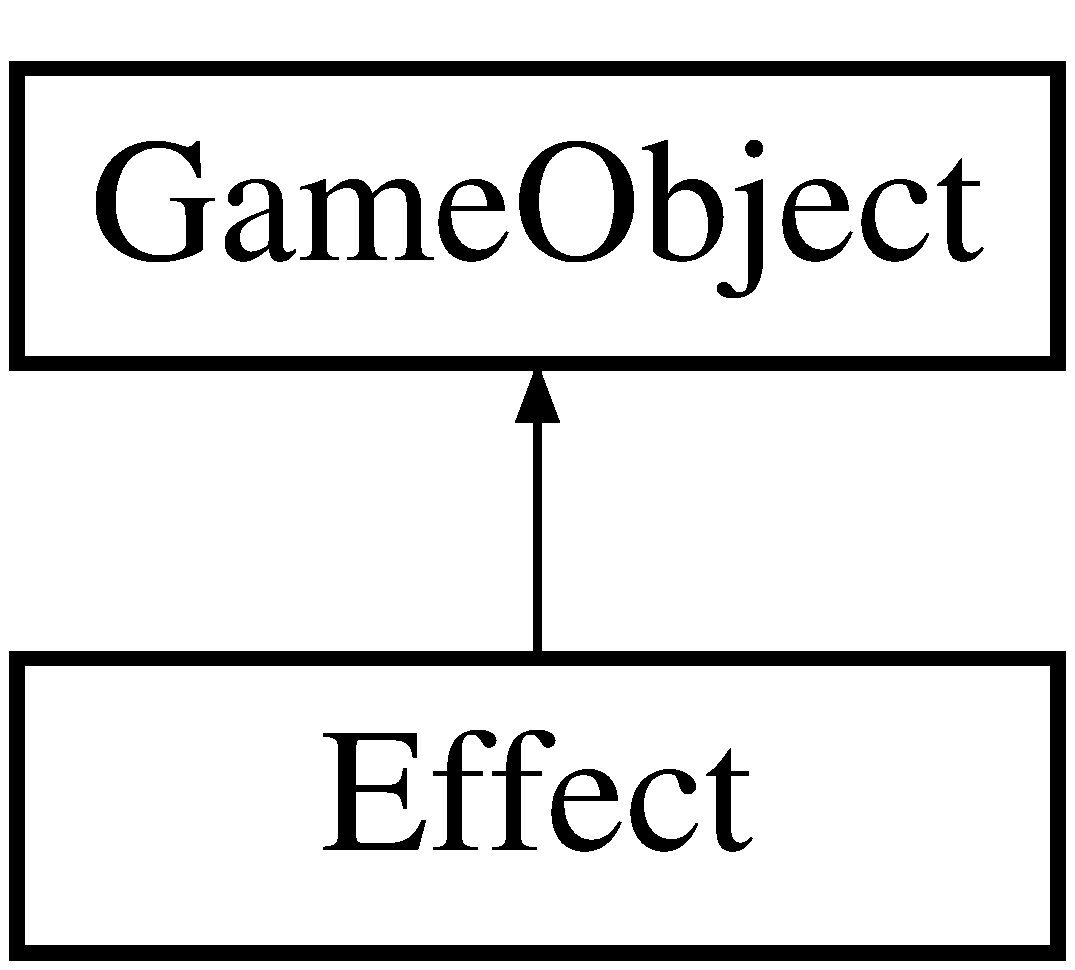
\includegraphics[height=2.000000cm]{class_effect}
\end{center}
\end{figure}
\subsection*{Public Member Functions}
\begin{DoxyCompactItemize}
\item 
\hyperlink{class_effect_a4dae74244f59936a49847da9217b4126}{Effect} ()
\begin{DoxyCompactList}\small\item\em \mbox{[}brief description\mbox{]} \end{DoxyCompactList}\item 
int \hyperlink{class_effect_a341dbd8ed4d921f21e041ad4c49f3ca5}{is\-Type} ()
\begin{DoxyCompactList}\small\item\em \mbox{[}brief description\mbox{]} \end{DoxyCompactList}\item 
void \hyperlink{class_effect_a8eef7dc5e13869286937eac91b6b4e82}{enable} (bool e)
\begin{DoxyCompactList}\small\item\em \mbox{[}brief description\mbox{]} \end{DoxyCompactList}\item 
bool \hyperlink{class_effect_a646edbd991706c9229ea1a87587a3ba3}{get\-Enable} ()
\begin{DoxyCompactList}\small\item\em \mbox{[}brief description\mbox{]} \end{DoxyCompactList}\item 
void \hyperlink{class_effect_a90509b57fed454734360a7bdad9e4441}{translate} (float x, float y, float z)
\begin{DoxyCompactList}\small\item\em \mbox{[}brief description\mbox{]} \end{DoxyCompactList}\item 
void \hyperlink{class_effect_a03da2911589ef11254c6ffd7ed0ca0ae}{set\-Pos} (float x, float y, float z)
\begin{DoxyCompactList}\small\item\em \mbox{[}brief description\mbox{]} \end{DoxyCompactList}\item 
\hyperlink{struct_vector3}{Vector3} \hyperlink{class_effect_a3439e1bf3ca53c04c408b94a5e62ceba}{get\-Pos} ()
\begin{DoxyCompactList}\small\item\em \mbox{[}brief description\mbox{]} \end{DoxyCompactList}\item 
float \hyperlink{class_effect_aacf6a5ad74b447aae18a18729c55a6f2}{get\-Pos\-X} ()
\begin{DoxyCompactList}\small\item\em \mbox{[}brief description\mbox{]} \end{DoxyCompactList}\item 
float \hyperlink{class_effect_a2ec270d5bf79b70e137e250abb115f55}{get\-Pos\-Y} ()
\begin{DoxyCompactList}\small\item\em \mbox{[}brief description\mbox{]} \end{DoxyCompactList}\item 
float \hyperlink{class_effect_a1dffa75aa0e151576d75882cf2ccfa9a}{get\-Pos\-Z} ()
\begin{DoxyCompactList}\small\item\em \mbox{[}brief description\mbox{]} \end{DoxyCompactList}\item 
void \hyperlink{class_effect_a1b58e2ce4a7bf8a8e5fbf19d60bc0f71}{set\-Script} (const char $\ast$file)
\begin{DoxyCompactList}\small\item\em \mbox{[}brief description\mbox{]} \end{DoxyCompactList}\item 
std\-::string \hyperlink{class_effect_a1fb8e7c630820f1313edfd120c661b38}{get\-Script} ()
\begin{DoxyCompactList}\small\item\em \mbox{[}brief description\mbox{]} \end{DoxyCompactList}\item 
\hypertarget{class_effect_ad9030a6b314f4a9e648908524fb83270}{std\-::string {\bfseries get\-Name} ()}\label{class_effect_ad9030a6b314f4a9e648908524fb83270}

\item 
\hypertarget{class_effect_a919b007b36957588ea56f835ef3acf37}{void {\bfseries set\-Name} (std\-::string n)}\label{class_effect_a919b007b36957588ea56f835ef3acf37}

\item 
\hypertarget{class_effect_a80b441abcfb87484c2ac01fafec7583c}{std\-::string {\bfseries get\-Texture} ()}\label{class_effect_a80b441abcfb87484c2ac01fafec7583c}

\item 
\hypertarget{class_effect_a06f9c033f26e418f9b4cc25d06e566ef}{void {\bfseries set\-Texture} (std\-::string t)}\label{class_effect_a06f9c033f26e418f9b4cc25d06e566ef}

\item 
\hypertarget{class_effect_aad6f7587068ecc284618c36e22a5a9fe}{float {\bfseries get\-Translate\-X} ()}\label{class_effect_aad6f7587068ecc284618c36e22a5a9fe}

\item 
\hypertarget{class_effect_a24280acf878697c283b659fa702d02f0}{float {\bfseries get\-Translate\-Y} ()}\label{class_effect_a24280acf878697c283b659fa702d02f0}

\item 
\hypertarget{class_effect_a3ca4ac0615dd911cbe815d9afef2cc15}{float {\bfseries get\-Translate\-Z} ()}\label{class_effect_a3ca4ac0615dd911cbe815d9afef2cc15}

\item 
\hypertarget{class_effect_ac7a5f58863d1ca0171a557e95afdf796}{void {\bfseries set\-Rotation} (Axis axis, float angle)}\label{class_effect_ac7a5f58863d1ca0171a557e95afdf796}

\item 
\hypertarget{class_effect_a5eb8688d83867718ae6ec63434ef1e72}{float {\bfseries get\-Rotation\-X} ()}\label{class_effect_a5eb8688d83867718ae6ec63434ef1e72}

\item 
\hypertarget{class_effect_aa15ba150e58d59861c4bdb2635682e14}{float {\bfseries get\-Rotation\-Y} ()}\label{class_effect_aa15ba150e58d59861c4bdb2635682e14}

\item 
\hypertarget{class_effect_a1f730389e0122a77b6a9dbf5cd2a2e74}{float {\bfseries get\-Rotation\-Z} ()}\label{class_effect_a1f730389e0122a77b6a9dbf5cd2a2e74}

\end{DoxyCompactItemize}
\subsection*{Additional Inherited Members}


\subsection{Detailed Description}
\mbox{[}brief description\mbox{]} 

\mbox{[}long description\mbox{]} \begin{DoxyReturn}{Returns}
\mbox{[}description\mbox{]} 
\end{DoxyReturn}
\begin{DoxyAuthor}{Author}
\mbox{[}author\mbox{]} 
\end{DoxyAuthor}


\subsection{Constructor \& Destructor Documentation}
\hypertarget{class_effect_a4dae74244f59936a49847da9217b4126}{\index{Effect@{Effect}!Effect@{Effect}}
\index{Effect@{Effect}!Effect@{Effect}}
\subsubsection[{Effect}]{\setlength{\rightskip}{0pt plus 5cm}Effect\-::\-Effect (
\begin{DoxyParamCaption}
{}
\end{DoxyParamCaption}
)}}\label{class_effect_a4dae74244f59936a49847da9217b4126}


\mbox{[}brief description\mbox{]} 

\mbox{[}long description\mbox{]} 

\subsection{Member Function Documentation}
\hypertarget{class_effect_a8eef7dc5e13869286937eac91b6b4e82}{\index{Effect@{Effect}!enable@{enable}}
\index{enable@{enable}!Effect@{Effect}}
\subsubsection[{enable}]{\setlength{\rightskip}{0pt plus 5cm}void Effect\-::enable (
\begin{DoxyParamCaption}
\item[{bool}]{e}
\end{DoxyParamCaption}
)\hspace{0.3cm}{\ttfamily [virtual]}}}\label{class_effect_a8eef7dc5e13869286937eac91b6b4e82}


\mbox{[}brief description\mbox{]} 

\mbox{[}long description\mbox{]}


\begin{DoxyParams}{Parameters}
{\em m} & \mbox{[}description\mbox{]} \\
\hline
{\em t} & \mbox{[}description\mbox{]} \\
\hline
\end{DoxyParams}


Implements \hyperlink{class_game_object_a5e7b5056ab92f998cda8fa3779bf44d1}{Game\-Object}.

\hypertarget{class_effect_a646edbd991706c9229ea1a87587a3ba3}{\index{Effect@{Effect}!get\-Enable@{get\-Enable}}
\index{get\-Enable@{get\-Enable}!Effect@{Effect}}
\subsubsection[{get\-Enable}]{\setlength{\rightskip}{0pt plus 5cm}bool Effect\-::get\-Enable (
\begin{DoxyParamCaption}
{}
\end{DoxyParamCaption}
)\hspace{0.3cm}{\ttfamily [virtual]}}}\label{class_effect_a646edbd991706c9229ea1a87587a3ba3}


\mbox{[}brief description\mbox{]} 

\mbox{[}long description\mbox{]}


\begin{DoxyParams}{Parameters}
{\em m} & \mbox{[}description\mbox{]} \\
\hline
{\em t} & \mbox{[}description\mbox{]} \\
\hline
\end{DoxyParams}


Implements \hyperlink{class_game_object_a0fa51b1d4bcf6756e4a5e1637fa01d78}{Game\-Object}.

\hypertarget{class_effect_a3439e1bf3ca53c04c408b94a5e62ceba}{\index{Effect@{Effect}!get\-Pos@{get\-Pos}}
\index{get\-Pos@{get\-Pos}!Effect@{Effect}}
\subsubsection[{get\-Pos}]{\setlength{\rightskip}{0pt plus 5cm}{\bf Vector3} Effect\-::get\-Pos (
\begin{DoxyParamCaption}
{}
\end{DoxyParamCaption}
)\hspace{0.3cm}{\ttfamily [virtual]}}}\label{class_effect_a3439e1bf3ca53c04c408b94a5e62ceba}


\mbox{[}brief description\mbox{]} 

\mbox{[}long description\mbox{]} \begin{DoxyReturn}{Returns}
\mbox{[}description\mbox{]} 
\end{DoxyReturn}


Implements \hyperlink{class_game_object_a01903e73800537f21d25040de96b1e0a}{Game\-Object}.

\hypertarget{class_effect_aacf6a5ad74b447aae18a18729c55a6f2}{\index{Effect@{Effect}!get\-Pos\-X@{get\-Pos\-X}}
\index{get\-Pos\-X@{get\-Pos\-X}!Effect@{Effect}}
\subsubsection[{get\-Pos\-X}]{\setlength{\rightskip}{0pt plus 5cm}float Effect\-::get\-Pos\-X (
\begin{DoxyParamCaption}
{}
\end{DoxyParamCaption}
)\hspace{0.3cm}{\ttfamily [virtual]}}}\label{class_effect_aacf6a5ad74b447aae18a18729c55a6f2}


\mbox{[}brief description\mbox{]} 

\mbox{[}long description\mbox{]} \begin{DoxyReturn}{Returns}
\mbox{[}description\mbox{]} 
\end{DoxyReturn}


Implements \hyperlink{class_game_object_ab41e4a13b4e37f7a40a9e5cf54db07d9}{Game\-Object}.

\hypertarget{class_effect_a2ec270d5bf79b70e137e250abb115f55}{\index{Effect@{Effect}!get\-Pos\-Y@{get\-Pos\-Y}}
\index{get\-Pos\-Y@{get\-Pos\-Y}!Effect@{Effect}}
\subsubsection[{get\-Pos\-Y}]{\setlength{\rightskip}{0pt plus 5cm}float Effect\-::get\-Pos\-Y (
\begin{DoxyParamCaption}
{}
\end{DoxyParamCaption}
)\hspace{0.3cm}{\ttfamily [virtual]}}}\label{class_effect_a2ec270d5bf79b70e137e250abb115f55}


\mbox{[}brief description\mbox{]} 

\mbox{[}long description\mbox{]} \begin{DoxyReturn}{Returns}
\mbox{[}description\mbox{]} 
\end{DoxyReturn}


Implements \hyperlink{class_game_object_aab59caeb6b903c23a76be1ddb1497a60}{Game\-Object}.

\hypertarget{class_effect_a1dffa75aa0e151576d75882cf2ccfa9a}{\index{Effect@{Effect}!get\-Pos\-Z@{get\-Pos\-Z}}
\index{get\-Pos\-Z@{get\-Pos\-Z}!Effect@{Effect}}
\subsubsection[{get\-Pos\-Z}]{\setlength{\rightskip}{0pt plus 5cm}float Effect\-::get\-Pos\-Z (
\begin{DoxyParamCaption}
{}
\end{DoxyParamCaption}
)\hspace{0.3cm}{\ttfamily [virtual]}}}\label{class_effect_a1dffa75aa0e151576d75882cf2ccfa9a}


\mbox{[}brief description\mbox{]} 

\mbox{[}long description\mbox{]} \begin{DoxyReturn}{Returns}
\mbox{[}description\mbox{]} 
\end{DoxyReturn}


Implements \hyperlink{class_game_object_a0eb3185aa4070664b4b7a6f23ae64f32}{Game\-Object}.

\hypertarget{class_effect_a1fb8e7c630820f1313edfd120c661b38}{\index{Effect@{Effect}!get\-Script@{get\-Script}}
\index{get\-Script@{get\-Script}!Effect@{Effect}}
\subsubsection[{get\-Script}]{\setlength{\rightskip}{0pt plus 5cm}std\-::string Effect\-::get\-Script (
\begin{DoxyParamCaption}
{}
\end{DoxyParamCaption}
)\hspace{0.3cm}{\ttfamily [virtual]}}}\label{class_effect_a1fb8e7c630820f1313edfd120c661b38}


\mbox{[}brief description\mbox{]} 

\mbox{[}long description\mbox{]} \begin{DoxyReturn}{Returns}
\mbox{[}description\mbox{]} 
\end{DoxyReturn}


Implements \hyperlink{class_game_object_af8c16297dbff83e1ae7c4f75f314b856}{Game\-Object}.

\hypertarget{class_effect_a341dbd8ed4d921f21e041ad4c49f3ca5}{\index{Effect@{Effect}!is\-Type@{is\-Type}}
\index{is\-Type@{is\-Type}!Effect@{Effect}}
\subsubsection[{is\-Type}]{\setlength{\rightskip}{0pt plus 5cm}int Effect\-::is\-Type (
\begin{DoxyParamCaption}
{}
\end{DoxyParamCaption}
)\hspace{0.3cm}{\ttfamily [virtual]}}}\label{class_effect_a341dbd8ed4d921f21e041ad4c49f3ca5}


\mbox{[}brief description\mbox{]} 

\mbox{[}long description\mbox{]} \begin{DoxyReturn}{Returns}
\mbox{[}description\mbox{]} 
\end{DoxyReturn}


Implements \hyperlink{class_game_object_a1d4237f8e511d5c6f0b1ad92480199b3}{Game\-Object}.

\hypertarget{class_effect_a03da2911589ef11254c6ffd7ed0ca0ae}{\index{Effect@{Effect}!set\-Pos@{set\-Pos}}
\index{set\-Pos@{set\-Pos}!Effect@{Effect}}
\subsubsection[{set\-Pos}]{\setlength{\rightskip}{0pt plus 5cm}void Effect\-::set\-Pos (
\begin{DoxyParamCaption}
\item[{float}]{x, }
\item[{float}]{y, }
\item[{float}]{z}
\end{DoxyParamCaption}
)\hspace{0.3cm}{\ttfamily [virtual]}}}\label{class_effect_a03da2911589ef11254c6ffd7ed0ca0ae}


\mbox{[}brief description\mbox{]} 

\mbox{[}long description\mbox{]}


\begin{DoxyParams}{Parameters}
{\em x} & \mbox{[}description\mbox{]} \\
\hline
{\em y} & \mbox{[}description\mbox{]} \\
\hline
{\em z} & \mbox{[}description\mbox{]} \\
\hline
\end{DoxyParams}


Implements \hyperlink{class_game_object_a6f33cf0e915855f22c7e115625138567}{Game\-Object}.

\hypertarget{class_effect_a1b58e2ce4a7bf8a8e5fbf19d60bc0f71}{\index{Effect@{Effect}!set\-Script@{set\-Script}}
\index{set\-Script@{set\-Script}!Effect@{Effect}}
\subsubsection[{set\-Script}]{\setlength{\rightskip}{0pt plus 5cm}void Effect\-::set\-Script (
\begin{DoxyParamCaption}
\item[{const char $\ast$}]{file}
\end{DoxyParamCaption}
)\hspace{0.3cm}{\ttfamily [virtual]}}}\label{class_effect_a1b58e2ce4a7bf8a8e5fbf19d60bc0f71}


\mbox{[}brief description\mbox{]} 

\mbox{[}long description\mbox{]}


\begin{DoxyParams}{Parameters}
{\em file} & \mbox{[}description\mbox{]} \\
\hline
\end{DoxyParams}


Implements \hyperlink{class_game_object_a3cdd9cb174d5fa4d4a5748df1ab09e87}{Game\-Object}.

\hypertarget{class_effect_a90509b57fed454734360a7bdad9e4441}{\index{Effect@{Effect}!translate@{translate}}
\index{translate@{translate}!Effect@{Effect}}
\subsubsection[{translate}]{\setlength{\rightskip}{0pt plus 5cm}void Effect\-::translate (
\begin{DoxyParamCaption}
\item[{float}]{x, }
\item[{float}]{y, }
\item[{float}]{z}
\end{DoxyParamCaption}
)\hspace{0.3cm}{\ttfamily [virtual]}}}\label{class_effect_a90509b57fed454734360a7bdad9e4441}


\mbox{[}brief description\mbox{]} 

\mbox{[}long description\mbox{]}


\begin{DoxyParams}{Parameters}
{\em x} & \mbox{[}description\mbox{]} \\
\hline
{\em y} & \mbox{[}description\mbox{]} \\
\hline
{\em z} & \mbox{[}description\mbox{]} \\
\hline
\end{DoxyParams}


Implements \hyperlink{class_game_object_a00ebf6691d90a55af08dd1b1afd7abaf}{Game\-Object}.



The documentation for this class was generated from the following files\-:\begin{DoxyCompactItemize}
\item 
E\-:/\-G\-R\-A\-B\-L\-A\-U\-R\-G/\-I\-S\-E/\-I\-S\-E-\/\-Demo/\-I\-S\-E-\/\-Demo/Game\-Object.\-h\item 
E\-:/\-G\-R\-A\-B\-L\-A\-U\-R\-G/\-I\-S\-E/\-I\-S\-E-\/\-Demo/\-I\-S\-E-\/\-Demo/Effect.\-cpp\end{DoxyCompactItemize}

\hypertarget{class_error}{\section{Error Class Reference}
\label{class_error}\index{Error@{Error}}
}
Inheritance diagram for Error\-:\begin{figure}[H]
\begin{center}
\leavevmode
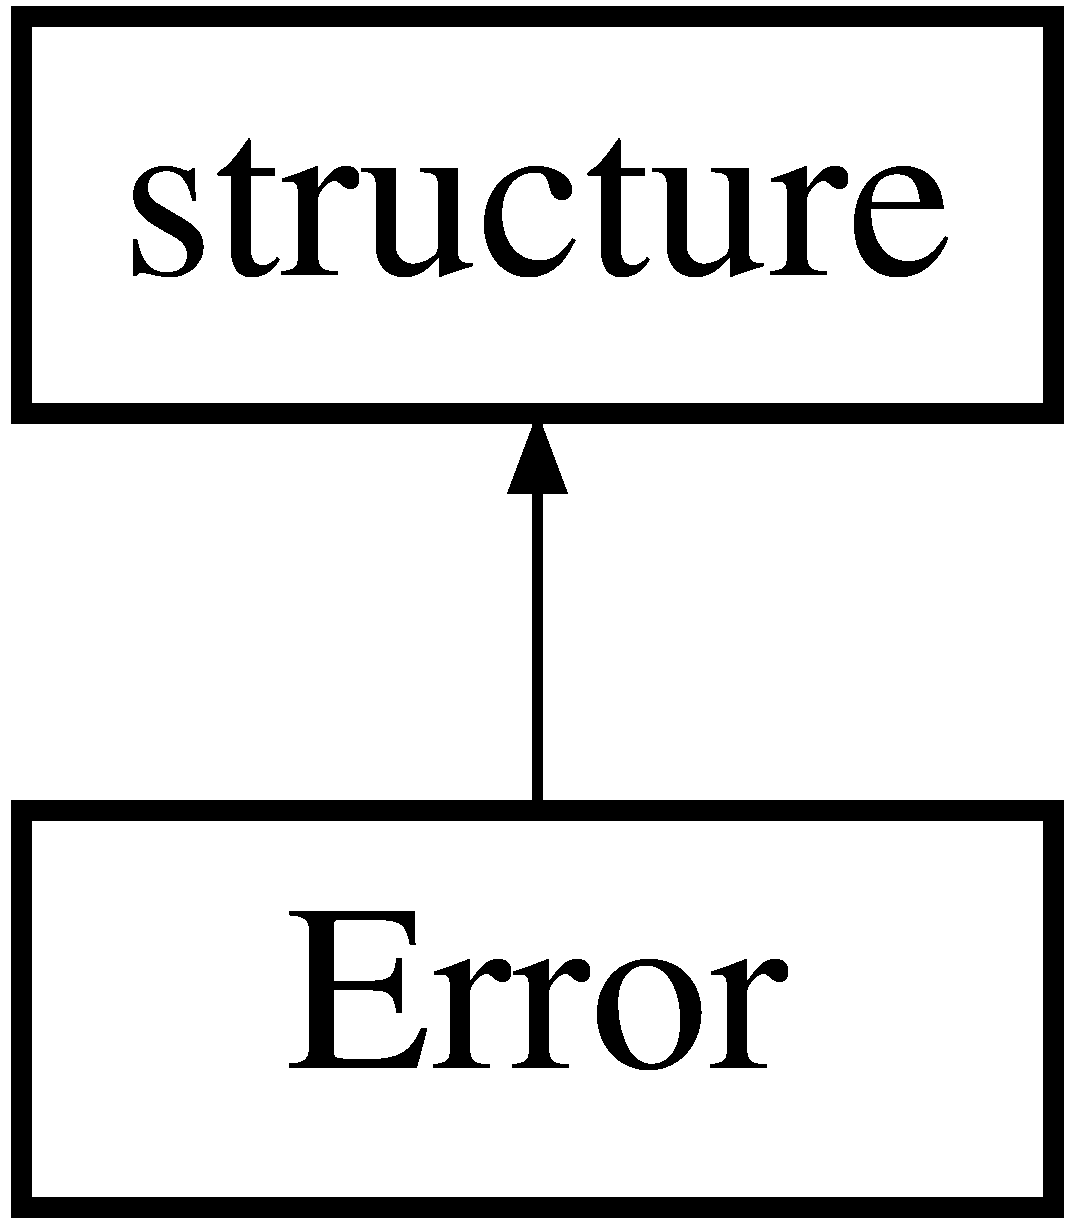
\includegraphics[height=2.000000cm]{class_error}
\end{center}
\end{figure}
\subsection*{Public Attributes}
\begin{DoxyCompactItemize}
\item 
\hypertarget{class_error_a7ca1958fd4898587d70b88c0c0dc0695}{std\-::string {\bfseries error}}\label{class_error_a7ca1958fd4898587d70b88c0c0dc0695}

\end{DoxyCompactItemize}


The documentation for this class was generated from the following file\-:\begin{DoxyCompactItemize}
\item 
E\-:/\-G\-R\-A\-B\-L\-A\-U\-R\-G/\-I\-S\-E/\-I\-S\-E-\/\-Demo/\-I\-S\-E-\/\-Demo/V\-A\-O.\-h\end{DoxyCompactItemize}

\hypertarget{class_game_object}{\section{Game\-Object Class Reference}
\label{class_game_object}\index{Game\-Object@{Game\-Object}}
}


\mbox{[}brief description\mbox{]}  




{\ttfamily \#include $<$Game\-Object.\-h$>$}

Inheritance diagram for Game\-Object\-:\begin{figure}[H]
\begin{center}
\leavevmode
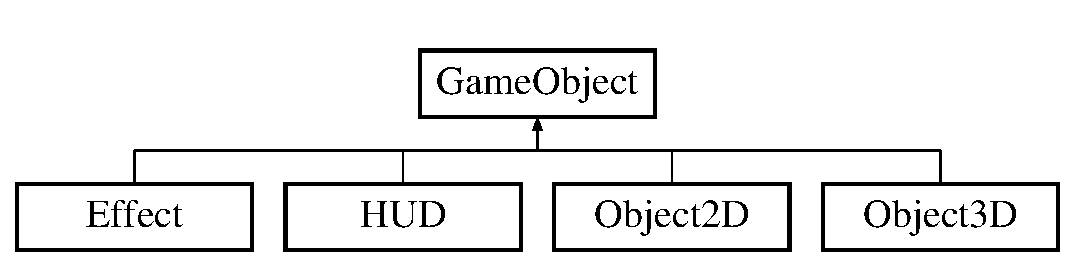
\includegraphics[height=2.000000cm]{class_game_object}
\end{center}
\end{figure}
\subsection*{Public Member Functions}
\begin{DoxyCompactItemize}
\item 
\hyperlink{class_game_object_a0348e3ee2e83d56eafca7a3547f432c4}{Game\-Object} ()
\begin{DoxyCompactList}\small\item\em \mbox{[}brief description\mbox{]} \end{DoxyCompactList}\item 
virtual void \hyperlink{class_game_object_a5e7b5056ab92f998cda8fa3779bf44d1}{enable} (bool e)=0
\begin{DoxyCompactList}\small\item\em \mbox{[}brief description\mbox{]} \end{DoxyCompactList}\item 
virtual bool \hyperlink{class_game_object_a0fa51b1d4bcf6756e4a5e1637fa01d78}{get\-Enable} ()=0
\begin{DoxyCompactList}\small\item\em \mbox{[}brief description\mbox{]} \end{DoxyCompactList}\item 
virtual int \hyperlink{class_game_object_a1d4237f8e511d5c6f0b1ad92480199b3}{is\-Type} ()=0
\begin{DoxyCompactList}\small\item\em \mbox{[}brief description\mbox{]} \end{DoxyCompactList}\item 
virtual void \hyperlink{class_game_object_a00ebf6691d90a55af08dd1b1afd7abaf}{translate} (float x, float y, float z)=0
\begin{DoxyCompactList}\small\item\em \mbox{[}brief description\mbox{]} \end{DoxyCompactList}\item 
virtual void \hyperlink{class_game_object_a6f33cf0e915855f22c7e115625138567}{set\-Pos} (float x, float y, float z)=0
\begin{DoxyCompactList}\small\item\em \mbox{[}brief description\mbox{]} \end{DoxyCompactList}\item 
virtual \hyperlink{struct_vector3}{Vector3} \hyperlink{class_game_object_a01903e73800537f21d25040de96b1e0a}{get\-Pos} ()=0
\begin{DoxyCompactList}\small\item\em \mbox{[}brief description\mbox{]} \end{DoxyCompactList}\item 
virtual float \hyperlink{class_game_object_ab41e4a13b4e37f7a40a9e5cf54db07d9}{get\-Pos\-X} ()=0
\begin{DoxyCompactList}\small\item\em \mbox{[}brief description\mbox{]} \end{DoxyCompactList}\item 
virtual float \hyperlink{class_game_object_aab59caeb6b903c23a76be1ddb1497a60}{get\-Pos\-Y} ()=0
\begin{DoxyCompactList}\small\item\em \mbox{[}brief description\mbox{]} \end{DoxyCompactList}\item 
virtual float \hyperlink{class_game_object_a0eb3185aa4070664b4b7a6f23ae64f32}{get\-Pos\-Z} ()=0
\begin{DoxyCompactList}\small\item\em \mbox{[}brief description\mbox{]} \end{DoxyCompactList}\item 
virtual void \hyperlink{class_game_object_a3cdd9cb174d5fa4d4a5748df1ab09e87}{set\-Script} (const char $\ast$file)=0
\begin{DoxyCompactList}\small\item\em \mbox{[}brief description\mbox{]} \end{DoxyCompactList}\item 
virtual std\-::string \hyperlink{class_game_object_af8c16297dbff83e1ae7c4f75f314b856}{get\-Script} ()=0
\begin{DoxyCompactList}\small\item\em \mbox{[}brief description\mbox{]} \end{DoxyCompactList}\item 
\hypertarget{class_game_object_a1157a25f56fbb0d748e0b21d0f4e0316}{virtual std\-::string {\bfseries get\-Name} ()=0}\label{class_game_object_a1157a25f56fbb0d748e0b21d0f4e0316}

\item 
\hypertarget{class_game_object_abc8fe45887eb41973b3c7880a599475f}{virtual void {\bfseries set\-Name} (std\-::string n)=0}\label{class_game_object_abc8fe45887eb41973b3c7880a599475f}

\item 
\hypertarget{class_game_object_a4f276ac2bb0e6820ebc22d2d79ed0d47}{virtual std\-::string {\bfseries get\-Texture} ()=0}\label{class_game_object_a4f276ac2bb0e6820ebc22d2d79ed0d47}

\item 
\hypertarget{class_game_object_a448191b3ecefd69425f3966792ac2bb9}{virtual void {\bfseries set\-Texture} (std\-::string t)=0}\label{class_game_object_a448191b3ecefd69425f3966792ac2bb9}

\item 
\hypertarget{class_game_object_a1d0422282bbb5f85bc6987ec46c6b276}{virtual float {\bfseries get\-Translate\-X} ()=0}\label{class_game_object_a1d0422282bbb5f85bc6987ec46c6b276}

\item 
\hypertarget{class_game_object_a22f094a0b08f06855ecbd17b9845ef50}{virtual float {\bfseries get\-Translate\-Y} ()=0}\label{class_game_object_a22f094a0b08f06855ecbd17b9845ef50}

\item 
\hypertarget{class_game_object_ac0efd129c13bf95753299fe85f97467a}{virtual float {\bfseries get\-Translate\-Z} ()=0}\label{class_game_object_ac0efd129c13bf95753299fe85f97467a}

\item 
\hypertarget{class_game_object_a1144922a11a0e343366a8a3fb8521725}{virtual void {\bfseries set\-Rotation} (Axis axis, float angle)=0}\label{class_game_object_a1144922a11a0e343366a8a3fb8521725}

\item 
\hypertarget{class_game_object_ab46716c3230c5d11eebff87c84ca22f5}{virtual float {\bfseries get\-Rotation\-X} ()=0}\label{class_game_object_ab46716c3230c5d11eebff87c84ca22f5}

\item 
\hypertarget{class_game_object_a6c98f336114110131ad3215409b23534}{virtual float {\bfseries get\-Rotation\-Y} ()=0}\label{class_game_object_a6c98f336114110131ad3215409b23534}

\item 
\hypertarget{class_game_object_ac377db42aef03de064f7bd06336a0be6}{virtual float {\bfseries get\-Rotation\-Z} ()=0}\label{class_game_object_ac377db42aef03de064f7bd06336a0be6}

\end{DoxyCompactItemize}
\subsection*{Protected Attributes}
\begin{DoxyCompactItemize}
\item 
\hypertarget{class_game_object_afd5103849de5f37ca335db6f3130ee82}{\hyperlink{struct_vector3}{Vector3} {\bfseries m\-\_\-pos}}\label{class_game_object_afd5103849de5f37ca335db6f3130ee82}

\item 
\hypertarget{class_game_object_a23ef635ddc2f31cb7598603bebe40606}{\hyperlink{struct_vector3}{Vector3} {\bfseries m\-\_\-translate}}\label{class_game_object_a23ef635ddc2f31cb7598603bebe40606}

\item 
\hypertarget{class_game_object_a6c819c0580be60c85aea1461b2b53d78}{\hyperlink{struct_vector3}{Vector3} {\bfseries m\-\_\-angle}}\label{class_game_object_a6c819c0580be60c85aea1461b2b53d78}

\item 
\hypertarget{class_game_object_a99c54e4fc64ef1fbdb94265073cb4922}{std\-::string {\bfseries m\-\_\-\-Script}}\label{class_game_object_a99c54e4fc64ef1fbdb94265073cb4922}

\item 
\hypertarget{class_game_object_afa7a039775a78a0ba3c0a4f03a1d12b9}{std\-::string {\bfseries m\-\_\-\-Name}}\label{class_game_object_afa7a039775a78a0ba3c0a4f03a1d12b9}

\item 
\hypertarget{class_game_object_a3d6c8380de814ab1c847cd7137fa1967}{std\-::string {\bfseries m\-\_\-\-Texture}}\label{class_game_object_a3d6c8380de814ab1c847cd7137fa1967}

\item 
\hypertarget{class_game_object_a45eabe6a1c3d55f65efeddf57c60e2c0}{bool {\bfseries m\-\_\-\-Enable}}\label{class_game_object_a45eabe6a1c3d55f65efeddf57c60e2c0}

\end{DoxyCompactItemize}


\subsection{Detailed Description}
\mbox{[}brief description\mbox{]} 

\mbox{[}long description\mbox{]} \begin{DoxyReturn}{Returns}
\mbox{[}description\mbox{]} 
\end{DoxyReturn}
\begin{DoxyAuthor}{Author}
\mbox{[}author\mbox{]} 
\end{DoxyAuthor}


\subsection{Constructor \& Destructor Documentation}
\hypertarget{class_game_object_a0348e3ee2e83d56eafca7a3547f432c4}{\index{Game\-Object@{Game\-Object}!Game\-Object@{Game\-Object}}
\index{Game\-Object@{Game\-Object}!GameObject@{Game\-Object}}
\subsubsection[{Game\-Object}]{\setlength{\rightskip}{0pt plus 5cm}Game\-Object\-::\-Game\-Object (
\begin{DoxyParamCaption}
{}
\end{DoxyParamCaption}
)}}\label{class_game_object_a0348e3ee2e83d56eafca7a3547f432c4}


\mbox{[}brief description\mbox{]} 

\mbox{[}long description\mbox{]} 

\subsection{Member Function Documentation}
\hypertarget{class_game_object_a5e7b5056ab92f998cda8fa3779bf44d1}{\index{Game\-Object@{Game\-Object}!enable@{enable}}
\index{enable@{enable}!GameObject@{Game\-Object}}
\subsubsection[{enable}]{\setlength{\rightskip}{0pt plus 5cm}virtual void Game\-Object\-::enable (
\begin{DoxyParamCaption}
\item[{bool}]{e}
\end{DoxyParamCaption}
)\hspace{0.3cm}{\ttfamily [pure virtual]}}}\label{class_game_object_a5e7b5056ab92f998cda8fa3779bf44d1}


\mbox{[}brief description\mbox{]} 

\mbox{[}long description\mbox{]}


\begin{DoxyParams}{Parameters}
{\em m} & \mbox{[}description\mbox{]} \\
\hline
{\em t} & \mbox{[}description\mbox{]} \\
\hline
\end{DoxyParams}


Implemented in \hyperlink{class_h_u_d_a680aa1c6c3562e75d8992e98c760c396}{H\-U\-D}, \hyperlink{class_effect_a8eef7dc5e13869286937eac91b6b4e82}{Effect}, \hyperlink{class_object3_d_a83b58f2bd94df5fb41cdd2ad2718b738}{Object3\-D}, and \hyperlink{class_object2_d_a5a2f5ce24ca8a271932fbdb86bc8aa8e}{Object2\-D}.

\hypertarget{class_game_object_a0fa51b1d4bcf6756e4a5e1637fa01d78}{\index{Game\-Object@{Game\-Object}!get\-Enable@{get\-Enable}}
\index{get\-Enable@{get\-Enable}!GameObject@{Game\-Object}}
\subsubsection[{get\-Enable}]{\setlength{\rightskip}{0pt plus 5cm}virtual bool Game\-Object\-::get\-Enable (
\begin{DoxyParamCaption}
{}
\end{DoxyParamCaption}
)\hspace{0.3cm}{\ttfamily [pure virtual]}}}\label{class_game_object_a0fa51b1d4bcf6756e4a5e1637fa01d78}


\mbox{[}brief description\mbox{]} 

\mbox{[}long description\mbox{]}


\begin{DoxyParams}{Parameters}
{\em m} & \mbox{[}description\mbox{]} \\
\hline
{\em t} & \mbox{[}description\mbox{]} \\
\hline
\end{DoxyParams}


Implemented in \hyperlink{class_h_u_d_a6a5223de11b980f618c1d668ba1e251e}{H\-U\-D}, \hyperlink{class_effect_a646edbd991706c9229ea1a87587a3ba3}{Effect}, \hyperlink{class_object3_d_ac51d638d70d1200d44d468945bfc0356}{Object3\-D}, and \hyperlink{class_object2_d_a8a36288b9032a3ae53cac87e37c66716}{Object2\-D}.

\hypertarget{class_game_object_a01903e73800537f21d25040de96b1e0a}{\index{Game\-Object@{Game\-Object}!get\-Pos@{get\-Pos}}
\index{get\-Pos@{get\-Pos}!GameObject@{Game\-Object}}
\subsubsection[{get\-Pos}]{\setlength{\rightskip}{0pt plus 5cm}virtual {\bf Vector3} Game\-Object\-::get\-Pos (
\begin{DoxyParamCaption}
{}
\end{DoxyParamCaption}
)\hspace{0.3cm}{\ttfamily [pure virtual]}}}\label{class_game_object_a01903e73800537f21d25040de96b1e0a}


\mbox{[}brief description\mbox{]} 

\mbox{[}long description\mbox{]} \begin{DoxyReturn}{Returns}
\mbox{[}description\mbox{]} 
\end{DoxyReturn}


Implemented in \hyperlink{class_h_u_d_a4894b3dfc5a21277a39466624fc3b820}{H\-U\-D}, \hyperlink{class_effect_a3439e1bf3ca53c04c408b94a5e62ceba}{Effect}, \hyperlink{class_object3_d_a7c4949df5017e162cd5921ed18061730}{Object3\-D}, and \hyperlink{class_object2_d_a4d74800b53451bfa94d89f4dfba3d00a}{Object2\-D}.

\hypertarget{class_game_object_ab41e4a13b4e37f7a40a9e5cf54db07d9}{\index{Game\-Object@{Game\-Object}!get\-Pos\-X@{get\-Pos\-X}}
\index{get\-Pos\-X@{get\-Pos\-X}!GameObject@{Game\-Object}}
\subsubsection[{get\-Pos\-X}]{\setlength{\rightskip}{0pt plus 5cm}virtual float Game\-Object\-::get\-Pos\-X (
\begin{DoxyParamCaption}
{}
\end{DoxyParamCaption}
)\hspace{0.3cm}{\ttfamily [pure virtual]}}}\label{class_game_object_ab41e4a13b4e37f7a40a9e5cf54db07d9}


\mbox{[}brief description\mbox{]} 

\mbox{[}long description\mbox{]} \begin{DoxyReturn}{Returns}
\mbox{[}description\mbox{]} 
\end{DoxyReturn}


Implemented in \hyperlink{class_h_u_d_ac1a3147a38bce30a51121929b45d2465}{H\-U\-D}, \hyperlink{class_effect_aacf6a5ad74b447aae18a18729c55a6f2}{Effect}, \hyperlink{class_object3_d_a76e35761a85a8660b078a3a4780c2525}{Object3\-D}, and \hyperlink{class_object2_d_a1e3b86ae9f6ab4c443ce12df0ef1730b}{Object2\-D}.

\hypertarget{class_game_object_aab59caeb6b903c23a76be1ddb1497a60}{\index{Game\-Object@{Game\-Object}!get\-Pos\-Y@{get\-Pos\-Y}}
\index{get\-Pos\-Y@{get\-Pos\-Y}!GameObject@{Game\-Object}}
\subsubsection[{get\-Pos\-Y}]{\setlength{\rightskip}{0pt plus 5cm}virtual float Game\-Object\-::get\-Pos\-Y (
\begin{DoxyParamCaption}
{}
\end{DoxyParamCaption}
)\hspace{0.3cm}{\ttfamily [pure virtual]}}}\label{class_game_object_aab59caeb6b903c23a76be1ddb1497a60}


\mbox{[}brief description\mbox{]} 

\mbox{[}long description\mbox{]} \begin{DoxyReturn}{Returns}
\mbox{[}description\mbox{]} 
\end{DoxyReturn}


Implemented in \hyperlink{class_h_u_d_a4891c528401f73e9b343a7d9ca46031e}{H\-U\-D}, \hyperlink{class_effect_a2ec270d5bf79b70e137e250abb115f55}{Effect}, \hyperlink{class_object3_d_a960a658a0c324bb13f5c230a52dabed9}{Object3\-D}, and \hyperlink{class_object2_d_a284eb150bf8c8ef6b383955302409a44}{Object2\-D}.

\hypertarget{class_game_object_a0eb3185aa4070664b4b7a6f23ae64f32}{\index{Game\-Object@{Game\-Object}!get\-Pos\-Z@{get\-Pos\-Z}}
\index{get\-Pos\-Z@{get\-Pos\-Z}!GameObject@{Game\-Object}}
\subsubsection[{get\-Pos\-Z}]{\setlength{\rightskip}{0pt plus 5cm}virtual float Game\-Object\-::get\-Pos\-Z (
\begin{DoxyParamCaption}
{}
\end{DoxyParamCaption}
)\hspace{0.3cm}{\ttfamily [pure virtual]}}}\label{class_game_object_a0eb3185aa4070664b4b7a6f23ae64f32}


\mbox{[}brief description\mbox{]} 

\mbox{[}long description\mbox{]} \begin{DoxyReturn}{Returns}
\mbox{[}description\mbox{]} 
\end{DoxyReturn}


Implemented in \hyperlink{class_h_u_d_a217856936008edbc9d885ab83a758be3}{H\-U\-D}, \hyperlink{class_effect_a1dffa75aa0e151576d75882cf2ccfa9a}{Effect}, \hyperlink{class_object3_d_a065ea3924cb5d9ba4fa70e2226d74e8d}{Object3\-D}, and \hyperlink{class_object2_d_a8a72705600b30cb9594c21aa66b219a0}{Object2\-D}.

\hypertarget{class_game_object_af8c16297dbff83e1ae7c4f75f314b856}{\index{Game\-Object@{Game\-Object}!get\-Script@{get\-Script}}
\index{get\-Script@{get\-Script}!GameObject@{Game\-Object}}
\subsubsection[{get\-Script}]{\setlength{\rightskip}{0pt plus 5cm}virtual std\-::string Game\-Object\-::get\-Script (
\begin{DoxyParamCaption}
{}
\end{DoxyParamCaption}
)\hspace{0.3cm}{\ttfamily [pure virtual]}}}\label{class_game_object_af8c16297dbff83e1ae7c4f75f314b856}


\mbox{[}brief description\mbox{]} 

\mbox{[}long description\mbox{]} \begin{DoxyReturn}{Returns}
\mbox{[}description\mbox{]} 
\end{DoxyReturn}


Implemented in \hyperlink{class_h_u_d_a135c55681055940941643fe9c11abeae}{H\-U\-D}, \hyperlink{class_effect_a1fb8e7c630820f1313edfd120c661b38}{Effect}, \hyperlink{class_object3_d_a9e3a956e808621d37029941057724fab}{Object3\-D}, and \hyperlink{class_object2_d_a953f9ebfc88c7d4ea4d155646c4f4a85}{Object2\-D}.

\hypertarget{class_game_object_a1d4237f8e511d5c6f0b1ad92480199b3}{\index{Game\-Object@{Game\-Object}!is\-Type@{is\-Type}}
\index{is\-Type@{is\-Type}!GameObject@{Game\-Object}}
\subsubsection[{is\-Type}]{\setlength{\rightskip}{0pt plus 5cm}virtual int Game\-Object\-::is\-Type (
\begin{DoxyParamCaption}
{}
\end{DoxyParamCaption}
)\hspace{0.3cm}{\ttfamily [pure virtual]}}}\label{class_game_object_a1d4237f8e511d5c6f0b1ad92480199b3}


\mbox{[}brief description\mbox{]} 

\mbox{[}long description\mbox{]} \begin{DoxyReturn}{Returns}
\mbox{[}description\mbox{]} 
\end{DoxyReturn}


Implemented in \hyperlink{class_h_u_d_a1f1b15d877fedfb447a0196bc26f150a}{H\-U\-D}, \hyperlink{class_effect_a341dbd8ed4d921f21e041ad4c49f3ca5}{Effect}, \hyperlink{class_object3_d_af9a973bc07b6dcdacefebe20023a1d51}{Object3\-D}, and \hyperlink{class_object2_d_abeb56d59b3bd118d9ba5f098bae0c763}{Object2\-D}.

\hypertarget{class_game_object_a6f33cf0e915855f22c7e115625138567}{\index{Game\-Object@{Game\-Object}!set\-Pos@{set\-Pos}}
\index{set\-Pos@{set\-Pos}!GameObject@{Game\-Object}}
\subsubsection[{set\-Pos}]{\setlength{\rightskip}{0pt plus 5cm}virtual void Game\-Object\-::set\-Pos (
\begin{DoxyParamCaption}
\item[{float}]{x, }
\item[{float}]{y, }
\item[{float}]{z}
\end{DoxyParamCaption}
)\hspace{0.3cm}{\ttfamily [pure virtual]}}}\label{class_game_object_a6f33cf0e915855f22c7e115625138567}


\mbox{[}brief description\mbox{]} 

\mbox{[}long description\mbox{]}


\begin{DoxyParams}{Parameters}
{\em x} & \mbox{[}description\mbox{]} \\
\hline
{\em y} & \mbox{[}description\mbox{]} \\
\hline
{\em z} & \mbox{[}description\mbox{]} \\
\hline
\end{DoxyParams}


Implemented in \hyperlink{class_h_u_d_a798eafd1edc326512a5dee73a09fd031}{H\-U\-D}, \hyperlink{class_effect_a03da2911589ef11254c6ffd7ed0ca0ae}{Effect}, \hyperlink{class_object3_d_a4913643d7f24106e2272e3cf6c49bb8e}{Object3\-D}, and \hyperlink{class_object2_d_ab07a1bb40355a3f4c0a46357aa51a132}{Object2\-D}.

\hypertarget{class_game_object_a3cdd9cb174d5fa4d4a5748df1ab09e87}{\index{Game\-Object@{Game\-Object}!set\-Script@{set\-Script}}
\index{set\-Script@{set\-Script}!GameObject@{Game\-Object}}
\subsubsection[{set\-Script}]{\setlength{\rightskip}{0pt plus 5cm}virtual void Game\-Object\-::set\-Script (
\begin{DoxyParamCaption}
\item[{const char $\ast$}]{file}
\end{DoxyParamCaption}
)\hspace{0.3cm}{\ttfamily [pure virtual]}}}\label{class_game_object_a3cdd9cb174d5fa4d4a5748df1ab09e87}


\mbox{[}brief description\mbox{]} 

\mbox{[}long description\mbox{]}


\begin{DoxyParams}{Parameters}
{\em file} & \mbox{[}description\mbox{]} \\
\hline
\end{DoxyParams}


Implemented in \hyperlink{class_h_u_d_a50588942ce8fbfe1690c4a39134606d7}{H\-U\-D}, \hyperlink{class_effect_a1b58e2ce4a7bf8a8e5fbf19d60bc0f71}{Effect}, \hyperlink{class_object3_d_a2f0bffd2963d34f7496531f35cfcb5ef}{Object3\-D}, and \hyperlink{class_object2_d_ae9379f6e64ee1d7661df355b91999d8d}{Object2\-D}.

\hypertarget{class_game_object_a00ebf6691d90a55af08dd1b1afd7abaf}{\index{Game\-Object@{Game\-Object}!translate@{translate}}
\index{translate@{translate}!GameObject@{Game\-Object}}
\subsubsection[{translate}]{\setlength{\rightskip}{0pt plus 5cm}virtual void Game\-Object\-::translate (
\begin{DoxyParamCaption}
\item[{float}]{x, }
\item[{float}]{y, }
\item[{float}]{z}
\end{DoxyParamCaption}
)\hspace{0.3cm}{\ttfamily [pure virtual]}}}\label{class_game_object_a00ebf6691d90a55af08dd1b1afd7abaf}


\mbox{[}brief description\mbox{]} 

\mbox{[}long description\mbox{]}


\begin{DoxyParams}{Parameters}
{\em x} & \mbox{[}description\mbox{]} \\
\hline
{\em y} & \mbox{[}description\mbox{]} \\
\hline
{\em z} & \mbox{[}description\mbox{]} \\
\hline
\end{DoxyParams}


Implemented in \hyperlink{class_h_u_d_a6bb647684d8c30cfa1e663549da37496}{H\-U\-D}, \hyperlink{class_effect_a90509b57fed454734360a7bdad9e4441}{Effect}, \hyperlink{class_object3_d_a1362e9e4752b6ce4bddb1fa69e0e0894}{Object3\-D}, and \hyperlink{class_object2_d_a2d47915dce9714aecbc03038ff408df7}{Object2\-D}.



The documentation for this class was generated from the following files\-:\begin{DoxyCompactItemize}
\item 
E\-:/\-G\-R\-A\-B\-L\-A\-U\-R\-G/\-I\-S\-E/\-I\-S\-E-\/\-Demo/\-I\-S\-E-\/\-Demo/Game\-Object.\-h\item 
E\-:/\-G\-R\-A\-B\-L\-A\-U\-R\-G/\-I\-S\-E/\-I\-S\-E-\/\-Demo/\-I\-S\-E-\/\-Demo/Gameobject.\-cpp\end{DoxyCompactItemize}

\hypertarget{class_game_object_factory}{\section{Game\-Object\-Factory Class Reference}
\label{class_game_object_factory}\index{Game\-Object\-Factory@{Game\-Object\-Factory}}
}


\mbox{[}brief description\mbox{]}  




{\ttfamily \#include $<$Game\-Object\-Factory.\-h$>$}

\subsection*{Public Types}
\begin{DoxyCompactItemize}
\item 
enum {\bfseries object\-Type} \{ {\bfseries O\-B\-J\-E\-C\-T2\-D} = 0, 
{\bfseries O\-B\-J\-E\-C\-T3\-D}, 
{\bfseries E\-F\-F\-E\-C\-T}, 
{\bfseries hud}
 \}
\end{DoxyCompactItemize}
\subsection*{Public Member Functions}
\begin{DoxyCompactItemize}
\item 
\hyperlink{class_game_object_factory_acb06c511e88956d6e47c28d026dc8ddd}{Game\-Object\-Factory} ()
\begin{DoxyCompactList}\small\item\em \mbox{[}brief description\mbox{]} \end{DoxyCompactList}\item 
\hyperlink{class_game_object}{Game\-Object} $\ast$ \hyperlink{class_game_object_factory_a5929bc6ad461c9668b478cf68bfd7311}{Create} (object\-Type ot)
\begin{DoxyCompactList}\small\item\em \mbox{[}brief description\mbox{]} \end{DoxyCompactList}\end{DoxyCompactItemize}


\subsection{Detailed Description}
\mbox{[}brief description\mbox{]} 

\mbox{[}long description\mbox{]} \begin{DoxyReturn}{Returns}
\mbox{[}description\mbox{]} 
\end{DoxyReturn}
\begin{DoxyAuthor}{Author}
\mbox{[}author\mbox{]} 
\end{DoxyAuthor}


\subsection{Constructor \& Destructor Documentation}
\hypertarget{class_game_object_factory_acb06c511e88956d6e47c28d026dc8ddd}{\index{Game\-Object\-Factory@{Game\-Object\-Factory}!Game\-Object\-Factory@{Game\-Object\-Factory}}
\index{Game\-Object\-Factory@{Game\-Object\-Factory}!GameObjectFactory@{Game\-Object\-Factory}}
\subsubsection[{Game\-Object\-Factory}]{\setlength{\rightskip}{0pt plus 5cm}Game\-Object\-Factory\-::\-Game\-Object\-Factory (
\begin{DoxyParamCaption}
{}
\end{DoxyParamCaption}
)}}\label{class_game_object_factory_acb06c511e88956d6e47c28d026dc8ddd}


\mbox{[}brief description\mbox{]} 

\mbox{[}long description\mbox{]} 

\subsection{Member Function Documentation}
\hypertarget{class_game_object_factory_a5929bc6ad461c9668b478cf68bfd7311}{\index{Game\-Object\-Factory@{Game\-Object\-Factory}!Create@{Create}}
\index{Create@{Create}!GameObjectFactory@{Game\-Object\-Factory}}
\subsubsection[{Create}]{\setlength{\rightskip}{0pt plus 5cm}{\bf Game\-Object} $\ast$ Game\-Object\-Factory\-::\-Create (
\begin{DoxyParamCaption}
\item[{object\-Type}]{ot}
\end{DoxyParamCaption}
)}}\label{class_game_object_factory_a5929bc6ad461c9668b478cf68bfd7311}


\mbox{[}brief description\mbox{]} 

\mbox{[}long description\mbox{]}


\begin{DoxyParams}{Parameters}
{\em ot} & \mbox{[}description\mbox{]} \\
\hline
\end{DoxyParams}
\begin{DoxyReturn}{Returns}
\mbox{[}description\mbox{]} 
\end{DoxyReturn}


The documentation for this class was generated from the following files\-:\begin{DoxyCompactItemize}
\item 
E\-:/\-G\-R\-A\-B\-L\-A\-U\-R\-G/\-I\-S\-E/\-I\-S\-E-\/\-Demo/\-I\-S\-E-\/\-Demo/Game\-Object\-Factory.\-h\item 
E\-:/\-G\-R\-A\-B\-L\-A\-U\-R\-G/\-I\-S\-E/\-I\-S\-E-\/\-Demo/\-I\-S\-E-\/\-Demo/Game\-Object\-Factory.\-cpp\end{DoxyCompactItemize}

\hypertarget{class_h_u_d}{\section{H\-U\-D Class Reference}
\label{class_h_u_d}\index{H\-U\-D@{H\-U\-D}}
}


\mbox{[}brief description\mbox{]}  




{\ttfamily \#include $<$Game\-Object.\-h$>$}

Inheritance diagram for H\-U\-D\-:\begin{figure}[H]
\begin{center}
\leavevmode
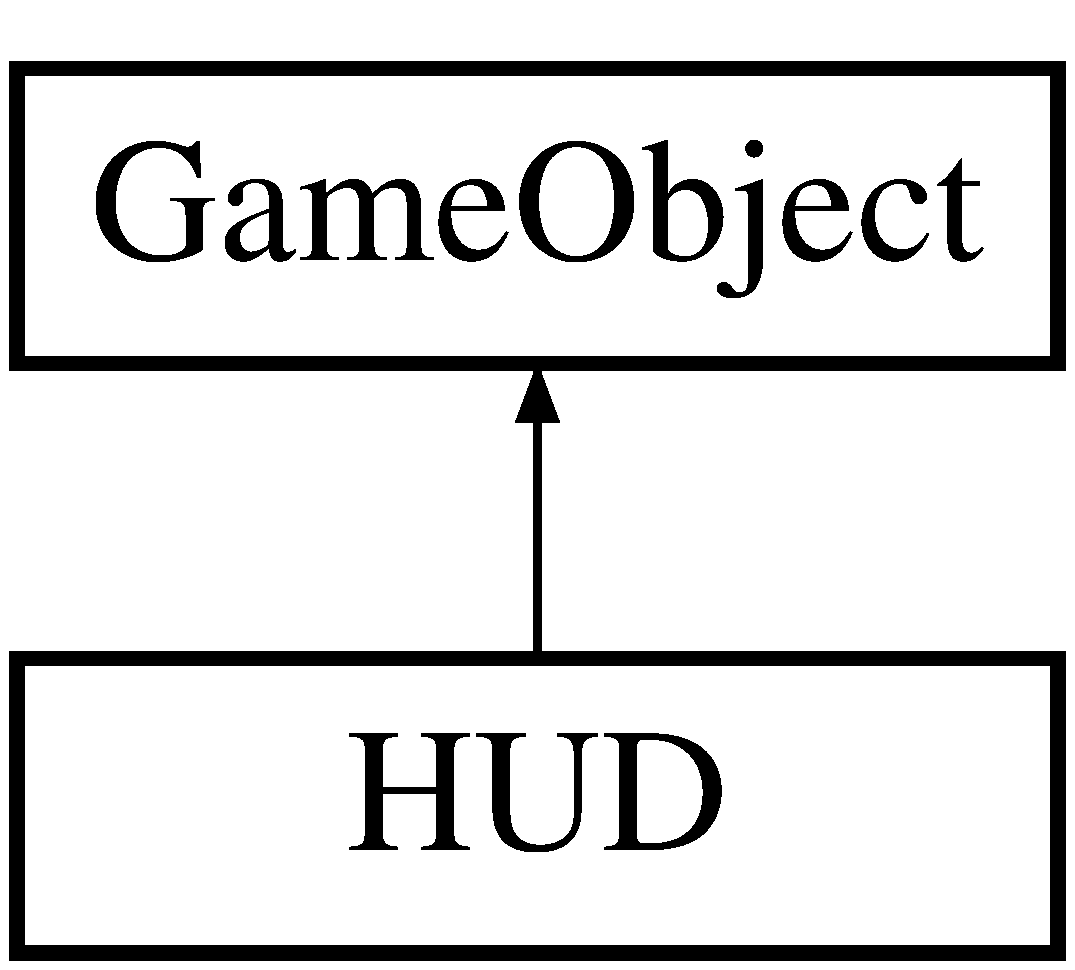
\includegraphics[height=2.000000cm]{class_h_u_d}
\end{center}
\end{figure}
\subsection*{Public Member Functions}
\begin{DoxyCompactItemize}
\item 
\hyperlink{class_h_u_d_a568b8ee1591f9ba3ed36ae05966f6b56}{H\-U\-D} ()
\begin{DoxyCompactList}\small\item\em \mbox{[}brief description\mbox{]} \end{DoxyCompactList}\item 
int \hyperlink{class_h_u_d_a1f1b15d877fedfb447a0196bc26f150a}{is\-Type} ()
\begin{DoxyCompactList}\small\item\em \mbox{[}brief description\mbox{]} \end{DoxyCompactList}\item 
void \hyperlink{class_h_u_d_a680aa1c6c3562e75d8992e98c760c396}{enable} (bool e)
\begin{DoxyCompactList}\small\item\em \mbox{[}brief description\mbox{]} \end{DoxyCompactList}\item 
bool \hyperlink{class_h_u_d_a6a5223de11b980f618c1d668ba1e251e}{get\-Enable} ()
\begin{DoxyCompactList}\small\item\em \mbox{[}brief description\mbox{]} \end{DoxyCompactList}\item 
void \hyperlink{class_h_u_d_a6bb647684d8c30cfa1e663549da37496}{translate} (float x, float y, float z)
\begin{DoxyCompactList}\small\item\em \mbox{[}brief description\mbox{]} \end{DoxyCompactList}\item 
void \hyperlink{class_h_u_d_a798eafd1edc326512a5dee73a09fd031}{set\-Pos} (float x, float y, float z)
\begin{DoxyCompactList}\small\item\em \mbox{[}brief description\mbox{]} \end{DoxyCompactList}\item 
\hyperlink{struct_vector3}{Vector3} \hyperlink{class_h_u_d_a4894b3dfc5a21277a39466624fc3b820}{get\-Pos} ()
\begin{DoxyCompactList}\small\item\em \mbox{[}brief description\mbox{]} \end{DoxyCompactList}\item 
float \hyperlink{class_h_u_d_ac1a3147a38bce30a51121929b45d2465}{get\-Pos\-X} ()
\begin{DoxyCompactList}\small\item\em \mbox{[}brief description\mbox{]} \end{DoxyCompactList}\item 
float \hyperlink{class_h_u_d_a4891c528401f73e9b343a7d9ca46031e}{get\-Pos\-Y} ()
\begin{DoxyCompactList}\small\item\em \mbox{[}brief description\mbox{]} \end{DoxyCompactList}\item 
float \hyperlink{class_h_u_d_a217856936008edbc9d885ab83a758be3}{get\-Pos\-Z} ()
\begin{DoxyCompactList}\small\item\em \mbox{[}brief description\mbox{]} \end{DoxyCompactList}\item 
void \hyperlink{class_h_u_d_a50588942ce8fbfe1690c4a39134606d7}{set\-Script} (const char $\ast$file)
\begin{DoxyCompactList}\small\item\em \mbox{[}brief description\mbox{]} \end{DoxyCompactList}\item 
std\-::string \hyperlink{class_h_u_d_a135c55681055940941643fe9c11abeae}{get\-Script} ()
\begin{DoxyCompactList}\small\item\em \mbox{[}brief description\mbox{]} \end{DoxyCompactList}\item 
\hypertarget{class_h_u_d_acec7f0a2b62edd40b6f2b7ffd99e4704}{std\-::string {\bfseries get\-Name} ()}\label{class_h_u_d_acec7f0a2b62edd40b6f2b7ffd99e4704}

\item 
\hypertarget{class_h_u_d_ad150c73b14f4433e9c1b0441d4e1a102}{void {\bfseries set\-Name} (std\-::string n)}\label{class_h_u_d_ad150c73b14f4433e9c1b0441d4e1a102}

\item 
\hypertarget{class_h_u_d_a244309dd23d2714db4ae6edf0591e040}{std\-::string {\bfseries get\-Texture} ()}\label{class_h_u_d_a244309dd23d2714db4ae6edf0591e040}

\item 
\hypertarget{class_h_u_d_ac69dae9ef6e44c7252482abb6e4877cc}{void {\bfseries set\-Texture} (std\-::string t)}\label{class_h_u_d_ac69dae9ef6e44c7252482abb6e4877cc}

\item 
\hypertarget{class_h_u_d_a1d8709e44f5b7fcefe5a338bebd689d8}{float {\bfseries get\-Translate\-X} ()}\label{class_h_u_d_a1d8709e44f5b7fcefe5a338bebd689d8}

\item 
\hypertarget{class_h_u_d_a7885a78f10b2e115a22d58a0ae93dfe8}{float {\bfseries get\-Translate\-Y} ()}\label{class_h_u_d_a7885a78f10b2e115a22d58a0ae93dfe8}

\item 
\hypertarget{class_h_u_d_abb85f040769e3d3394a1ab3d13eb710d}{float {\bfseries get\-Translate\-Z} ()}\label{class_h_u_d_abb85f040769e3d3394a1ab3d13eb710d}

\item 
\hypertarget{class_h_u_d_af102f097d1bd88a6592250b1d36c9b45}{void {\bfseries set\-Rotation} (Axis axis, float angle)}\label{class_h_u_d_af102f097d1bd88a6592250b1d36c9b45}

\item 
\hypertarget{class_h_u_d_a2ab2a6e8b81ccb700d664c0357d9370b}{float {\bfseries get\-Rotation\-X} ()}\label{class_h_u_d_a2ab2a6e8b81ccb700d664c0357d9370b}

\item 
\hypertarget{class_h_u_d_a86c4c0ddc76f0b2f21fa919d59d443f4}{float {\bfseries get\-Rotation\-Y} ()}\label{class_h_u_d_a86c4c0ddc76f0b2f21fa919d59d443f4}

\item 
\hypertarget{class_h_u_d_a52e54a745af110884f7af992fb3dc313}{float {\bfseries get\-Rotation\-Z} ()}\label{class_h_u_d_a52e54a745af110884f7af992fb3dc313}

\end{DoxyCompactItemize}
\subsection*{Additional Inherited Members}


\subsection{Detailed Description}
\mbox{[}brief description\mbox{]} 

\mbox{[}long description\mbox{]} \begin{DoxyReturn}{Returns}
\mbox{[}description\mbox{]} 
\end{DoxyReturn}
\begin{DoxyAuthor}{Author}
\mbox{[}author\mbox{]} 
\end{DoxyAuthor}


\subsection{Constructor \& Destructor Documentation}
\hypertarget{class_h_u_d_a568b8ee1591f9ba3ed36ae05966f6b56}{\index{H\-U\-D@{H\-U\-D}!H\-U\-D@{H\-U\-D}}
\index{H\-U\-D@{H\-U\-D}!HUD@{H\-U\-D}}
\subsubsection[{H\-U\-D}]{\setlength{\rightskip}{0pt plus 5cm}H\-U\-D\-::\-H\-U\-D (
\begin{DoxyParamCaption}
{}
\end{DoxyParamCaption}
)}}\label{class_h_u_d_a568b8ee1591f9ba3ed36ae05966f6b56}


\mbox{[}brief description\mbox{]} 

\mbox{[}long description\mbox{]} 

\subsection{Member Function Documentation}
\hypertarget{class_h_u_d_a680aa1c6c3562e75d8992e98c760c396}{\index{H\-U\-D@{H\-U\-D}!enable@{enable}}
\index{enable@{enable}!HUD@{H\-U\-D}}
\subsubsection[{enable}]{\setlength{\rightskip}{0pt plus 5cm}void H\-U\-D\-::enable (
\begin{DoxyParamCaption}
\item[{bool}]{e}
\end{DoxyParamCaption}
)\hspace{0.3cm}{\ttfamily [virtual]}}}\label{class_h_u_d_a680aa1c6c3562e75d8992e98c760c396}


\mbox{[}brief description\mbox{]} 

\mbox{[}long description\mbox{]}


\begin{DoxyParams}{Parameters}
{\em m} & \mbox{[}description\mbox{]} \\
\hline
{\em t} & \mbox{[}description\mbox{]} \\
\hline
\end{DoxyParams}


Implements \hyperlink{class_game_object_a5e7b5056ab92f998cda8fa3779bf44d1}{Game\-Object}.

\hypertarget{class_h_u_d_a6a5223de11b980f618c1d668ba1e251e}{\index{H\-U\-D@{H\-U\-D}!get\-Enable@{get\-Enable}}
\index{get\-Enable@{get\-Enable}!HUD@{H\-U\-D}}
\subsubsection[{get\-Enable}]{\setlength{\rightskip}{0pt plus 5cm}bool H\-U\-D\-::get\-Enable (
\begin{DoxyParamCaption}
{}
\end{DoxyParamCaption}
)\hspace{0.3cm}{\ttfamily [virtual]}}}\label{class_h_u_d_a6a5223de11b980f618c1d668ba1e251e}


\mbox{[}brief description\mbox{]} 

\mbox{[}long description\mbox{]}


\begin{DoxyParams}{Parameters}
{\em m} & \mbox{[}description\mbox{]} \\
\hline
{\em t} & \mbox{[}description\mbox{]} \\
\hline
\end{DoxyParams}


Implements \hyperlink{class_game_object_a0fa51b1d4bcf6756e4a5e1637fa01d78}{Game\-Object}.

\hypertarget{class_h_u_d_a4894b3dfc5a21277a39466624fc3b820}{\index{H\-U\-D@{H\-U\-D}!get\-Pos@{get\-Pos}}
\index{get\-Pos@{get\-Pos}!HUD@{H\-U\-D}}
\subsubsection[{get\-Pos}]{\setlength{\rightskip}{0pt plus 5cm}{\bf Vector3} H\-U\-D\-::get\-Pos (
\begin{DoxyParamCaption}
{}
\end{DoxyParamCaption}
)\hspace{0.3cm}{\ttfamily [virtual]}}}\label{class_h_u_d_a4894b3dfc5a21277a39466624fc3b820}


\mbox{[}brief description\mbox{]} 

\mbox{[}long description\mbox{]} \begin{DoxyReturn}{Returns}
\mbox{[}description\mbox{]} 
\end{DoxyReturn}


Implements \hyperlink{class_game_object_a01903e73800537f21d25040de96b1e0a}{Game\-Object}.

\hypertarget{class_h_u_d_ac1a3147a38bce30a51121929b45d2465}{\index{H\-U\-D@{H\-U\-D}!get\-Pos\-X@{get\-Pos\-X}}
\index{get\-Pos\-X@{get\-Pos\-X}!HUD@{H\-U\-D}}
\subsubsection[{get\-Pos\-X}]{\setlength{\rightskip}{0pt plus 5cm}float H\-U\-D\-::get\-Pos\-X (
\begin{DoxyParamCaption}
{}
\end{DoxyParamCaption}
)\hspace{0.3cm}{\ttfamily [virtual]}}}\label{class_h_u_d_ac1a3147a38bce30a51121929b45d2465}


\mbox{[}brief description\mbox{]} 

\mbox{[}long description\mbox{]} \begin{DoxyReturn}{Returns}
\mbox{[}description\mbox{]} 
\end{DoxyReturn}


Implements \hyperlink{class_game_object_ab41e4a13b4e37f7a40a9e5cf54db07d9}{Game\-Object}.

\hypertarget{class_h_u_d_a4891c528401f73e9b343a7d9ca46031e}{\index{H\-U\-D@{H\-U\-D}!get\-Pos\-Y@{get\-Pos\-Y}}
\index{get\-Pos\-Y@{get\-Pos\-Y}!HUD@{H\-U\-D}}
\subsubsection[{get\-Pos\-Y}]{\setlength{\rightskip}{0pt plus 5cm}float H\-U\-D\-::get\-Pos\-Y (
\begin{DoxyParamCaption}
{}
\end{DoxyParamCaption}
)\hspace{0.3cm}{\ttfamily [virtual]}}}\label{class_h_u_d_a4891c528401f73e9b343a7d9ca46031e}


\mbox{[}brief description\mbox{]} 

\mbox{[}long description\mbox{]} \begin{DoxyReturn}{Returns}
\mbox{[}description\mbox{]} 
\end{DoxyReturn}


Implements \hyperlink{class_game_object_aab59caeb6b903c23a76be1ddb1497a60}{Game\-Object}.

\hypertarget{class_h_u_d_a217856936008edbc9d885ab83a758be3}{\index{H\-U\-D@{H\-U\-D}!get\-Pos\-Z@{get\-Pos\-Z}}
\index{get\-Pos\-Z@{get\-Pos\-Z}!HUD@{H\-U\-D}}
\subsubsection[{get\-Pos\-Z}]{\setlength{\rightskip}{0pt plus 5cm}float H\-U\-D\-::get\-Pos\-Z (
\begin{DoxyParamCaption}
{}
\end{DoxyParamCaption}
)\hspace{0.3cm}{\ttfamily [virtual]}}}\label{class_h_u_d_a217856936008edbc9d885ab83a758be3}


\mbox{[}brief description\mbox{]} 

\mbox{[}long description\mbox{]} \begin{DoxyReturn}{Returns}
\mbox{[}description\mbox{]} 
\end{DoxyReturn}


Implements \hyperlink{class_game_object_a0eb3185aa4070664b4b7a6f23ae64f32}{Game\-Object}.

\hypertarget{class_h_u_d_a135c55681055940941643fe9c11abeae}{\index{H\-U\-D@{H\-U\-D}!get\-Script@{get\-Script}}
\index{get\-Script@{get\-Script}!HUD@{H\-U\-D}}
\subsubsection[{get\-Script}]{\setlength{\rightskip}{0pt plus 5cm}std\-::string H\-U\-D\-::get\-Script (
\begin{DoxyParamCaption}
{}
\end{DoxyParamCaption}
)\hspace{0.3cm}{\ttfamily [virtual]}}}\label{class_h_u_d_a135c55681055940941643fe9c11abeae}


\mbox{[}brief description\mbox{]} 

\mbox{[}long description\mbox{]} \begin{DoxyReturn}{Returns}
\mbox{[}description\mbox{]} 
\end{DoxyReturn}


Implements \hyperlink{class_game_object_af8c16297dbff83e1ae7c4f75f314b856}{Game\-Object}.

\hypertarget{class_h_u_d_a1f1b15d877fedfb447a0196bc26f150a}{\index{H\-U\-D@{H\-U\-D}!is\-Type@{is\-Type}}
\index{is\-Type@{is\-Type}!HUD@{H\-U\-D}}
\subsubsection[{is\-Type}]{\setlength{\rightskip}{0pt plus 5cm}int H\-U\-D\-::is\-Type (
\begin{DoxyParamCaption}
{}
\end{DoxyParamCaption}
)\hspace{0.3cm}{\ttfamily [virtual]}}}\label{class_h_u_d_a1f1b15d877fedfb447a0196bc26f150a}


\mbox{[}brief description\mbox{]} 

\mbox{[}long description\mbox{]} \begin{DoxyReturn}{Returns}
\mbox{[}description\mbox{]} 
\end{DoxyReturn}


Implements \hyperlink{class_game_object_a1d4237f8e511d5c6f0b1ad92480199b3}{Game\-Object}.

\hypertarget{class_h_u_d_a798eafd1edc326512a5dee73a09fd031}{\index{H\-U\-D@{H\-U\-D}!set\-Pos@{set\-Pos}}
\index{set\-Pos@{set\-Pos}!HUD@{H\-U\-D}}
\subsubsection[{set\-Pos}]{\setlength{\rightskip}{0pt plus 5cm}void H\-U\-D\-::set\-Pos (
\begin{DoxyParamCaption}
\item[{float}]{x, }
\item[{float}]{y, }
\item[{float}]{z}
\end{DoxyParamCaption}
)\hspace{0.3cm}{\ttfamily [virtual]}}}\label{class_h_u_d_a798eafd1edc326512a5dee73a09fd031}


\mbox{[}brief description\mbox{]} 

\mbox{[}long description\mbox{]}


\begin{DoxyParams}{Parameters}
{\em x} & \mbox{[}description\mbox{]} \\
\hline
{\em y} & \mbox{[}description\mbox{]} \\
\hline
{\em z} & \mbox{[}description\mbox{]} \\
\hline
\end{DoxyParams}


Implements \hyperlink{class_game_object_a6f33cf0e915855f22c7e115625138567}{Game\-Object}.

\hypertarget{class_h_u_d_a50588942ce8fbfe1690c4a39134606d7}{\index{H\-U\-D@{H\-U\-D}!set\-Script@{set\-Script}}
\index{set\-Script@{set\-Script}!HUD@{H\-U\-D}}
\subsubsection[{set\-Script}]{\setlength{\rightskip}{0pt plus 5cm}void H\-U\-D\-::set\-Script (
\begin{DoxyParamCaption}
\item[{const char $\ast$}]{file}
\end{DoxyParamCaption}
)\hspace{0.3cm}{\ttfamily [virtual]}}}\label{class_h_u_d_a50588942ce8fbfe1690c4a39134606d7}


\mbox{[}brief description\mbox{]} 

\mbox{[}long description\mbox{]}


\begin{DoxyParams}{Parameters}
{\em file} & \mbox{[}description\mbox{]} \\
\hline
\end{DoxyParams}


Implements \hyperlink{class_game_object_a3cdd9cb174d5fa4d4a5748df1ab09e87}{Game\-Object}.

\hypertarget{class_h_u_d_a6bb647684d8c30cfa1e663549da37496}{\index{H\-U\-D@{H\-U\-D}!translate@{translate}}
\index{translate@{translate}!HUD@{H\-U\-D}}
\subsubsection[{translate}]{\setlength{\rightskip}{0pt plus 5cm}void H\-U\-D\-::translate (
\begin{DoxyParamCaption}
\item[{float}]{x, }
\item[{float}]{y, }
\item[{float}]{z}
\end{DoxyParamCaption}
)\hspace{0.3cm}{\ttfamily [virtual]}}}\label{class_h_u_d_a6bb647684d8c30cfa1e663549da37496}


\mbox{[}brief description\mbox{]} 

\mbox{[}long description\mbox{]}


\begin{DoxyParams}{Parameters}
{\em x} & \mbox{[}description\mbox{]} \\
\hline
{\em y} & \mbox{[}description\mbox{]} \\
\hline
{\em z} & \mbox{[}description\mbox{]} \\
\hline
\end{DoxyParams}


Implements \hyperlink{class_game_object_a00ebf6691d90a55af08dd1b1afd7abaf}{Game\-Object}.



The documentation for this class was generated from the following files\-:\begin{DoxyCompactItemize}
\item 
E\-:/\-G\-R\-A\-B\-L\-A\-U\-R\-G/\-I\-S\-E/\-I\-S\-E-\/\-Demo/\-I\-S\-E-\/\-Demo/Game\-Object.\-h\item 
E\-:/\-G\-R\-A\-B\-L\-A\-U\-R\-G/\-I\-S\-E/\-I\-S\-E-\/\-Demo/\-I\-S\-E-\/\-Demo/H\-U\-D.\-cpp\end{DoxyCompactItemize}

\hypertarget{class_input}{\section{Input Class Reference}
\label{class_input}\index{Input@{Input}}
}


The input class.  




{\ttfamily \#include $<$Input.\-h$>$}

\subsection*{Public Member Functions}
\begin{DoxyCompactItemize}
\item 
bool \hyperlink{class_input_a9f5845c6e557825117e57455f97bf557}{is\-Press} (Keyboard\-::\-Key key)
\begin{DoxyCompactList}\small\item\em check is a key is pressed \end{DoxyCompactList}\item 
bool \hyperlink{class_input_aadcf0bcc21873a7bb1ac6e54f74d7c76}{is\-Released} (Keyboard\-::\-Key key)
\begin{DoxyCompactList}\small\item\em check if a key has been released (once occurs once after a press) \end{DoxyCompactList}\item 
bool \hyperlink{class_input_ae263e207d1f27420a393054f60ce4f67}{is\-Mouse\-Press} (Mouse\-::\-Button but)
\begin{DoxyCompactList}\small\item\em check if a mouse button has been pressed \end{DoxyCompactList}\item 
bool \hyperlink{class_input_a049d3da4ae94d9e3ebb522d9dd3eb5de}{is\-Mouse\-Released} (Mouse\-::\-Button but)
\begin{DoxyCompactList}\small\item\em check if a mouse button has been released \end{DoxyCompactList}\item 
void \hyperlink{class_input_ad540f1ea1157518fcfc51ba303913dce}{lock\-Mouse} ()
\begin{DoxyCompactList}\small\item\em lock the mouse in a position \end{DoxyCompactList}\item 
void \hyperlink{class_input_a2af99e8e16adb1d99684edf8b77e53ea}{release\-Mouse} ()
\begin{DoxyCompactList}\small\item\em release the mouse from its lock \end{DoxyCompactList}\item 
void \hyperlink{class_input_aae244dc7ffdd7736b1c8660631c51793}{set\-Mouse\-Lock\-Position} (int x, int y)
\begin{DoxyCompactList}\small\item\em Set the mouse lock position. \end{DoxyCompactList}\item 
void \hyperlink{class_input_adb2a5b2e67f5516254b515675ed99a46}{get\-Mouse\-Location} (int \&x, int \&y)
\begin{DoxyCompactList}\small\item\em get the current mouse location \end{DoxyCompactList}\item 
void \hyperlink{class_input_a6739e45b765de931e931c2048bed6cb1}{get\-Mouse\-Vec} (int \&x, int \&y)
\begin{DoxyCompactList}\small\item\em get the difference in movement from one call to the next \end{DoxyCompactList}\item 
void \hyperlink{class_input_a4491443d2a0c9e8c562d798d38017651}{mouse\-Update} ()
\begin{DoxyCompactList}\small\item\em Call to keep the mouse function good. \end{DoxyCompactList}\end{DoxyCompactItemize}


\subsection{Detailed Description}
The input class. 

This is the engine it takes in the inputs from other parts and puts them into an eays to work with file.

\begin{DoxyAuthor}{Author}
Umar Badat 
\end{DoxyAuthor}
\begin{DoxyNote}{Note}
store the input and can keep track of when a button is releaed (only occurs once after it has been pressed) 
\end{DoxyNote}


\subsection{Member Function Documentation}
\hypertarget{class_input_adb2a5b2e67f5516254b515675ed99a46}{\index{Input@{Input}!get\-Mouse\-Location@{get\-Mouse\-Location}}
\index{get\-Mouse\-Location@{get\-Mouse\-Location}!Input@{Input}}
\subsubsection[{get\-Mouse\-Location}]{\setlength{\rightskip}{0pt plus 5cm}void Input\-::get\-Mouse\-Location (
\begin{DoxyParamCaption}
\item[{int \&}]{x, }
\item[{int \&}]{y}
\end{DoxyParamCaption}
)}}\label{class_input_adb2a5b2e67f5516254b515675ed99a46}


get the current mouse location 

Get the current mouse location in windows space (not relative to your window)


\begin{DoxyParams}{Parameters}
{\em x} & address of an int, x is then assigned \\
\hline
{\em y} & address of an int, y is then assigned \\
\hline
\end{DoxyParams}
\hypertarget{class_input_a6739e45b765de931e931c2048bed6cb1}{\index{Input@{Input}!get\-Mouse\-Vec@{get\-Mouse\-Vec}}
\index{get\-Mouse\-Vec@{get\-Mouse\-Vec}!Input@{Input}}
\subsubsection[{get\-Mouse\-Vec}]{\setlength{\rightskip}{0pt plus 5cm}void Input\-::get\-Mouse\-Vec (
\begin{DoxyParamCaption}
\item[{int \&}]{x, }
\item[{int \&}]{y}
\end{DoxyParamCaption}
)}}\label{class_input_a6739e45b765de931e931c2048bed6cb1}


get the difference in movement from one call to the next 

get the vector of a movement of the mouse from one call to the next


\begin{DoxyParams}{Parameters}
{\em x} & address x gives the mouses x position \\
\hline
{\em y} & address y gives the mouses y position \\
\hline
\end{DoxyParams}
\hypertarget{class_input_ae263e207d1f27420a393054f60ce4f67}{\index{Input@{Input}!is\-Mouse\-Press@{is\-Mouse\-Press}}
\index{is\-Mouse\-Press@{is\-Mouse\-Press}!Input@{Input}}
\subsubsection[{is\-Mouse\-Press}]{\setlength{\rightskip}{0pt plus 5cm}bool Input\-::is\-Mouse\-Press (
\begin{DoxyParamCaption}
\item[{Mouse\-::\-Button}]{but}
\end{DoxyParamCaption}
)}}\label{class_input_ae263e207d1f27420a393054f60ce4f67}


check if a mouse button has been pressed 

Check if a mouse button has been pressed


\begin{DoxyParams}{Parameters}
{\em but} & enum representing a key \\
\hline
\end{DoxyParams}
\begin{DoxyReturn}{Returns}
true if the button is being pressed 
\end{DoxyReturn}
\hypertarget{class_input_a049d3da4ae94d9e3ebb522d9dd3eb5de}{\index{Input@{Input}!is\-Mouse\-Released@{is\-Mouse\-Released}}
\index{is\-Mouse\-Released@{is\-Mouse\-Released}!Input@{Input}}
\subsubsection[{is\-Mouse\-Released}]{\setlength{\rightskip}{0pt plus 5cm}bool Input\-::is\-Mouse\-Released (
\begin{DoxyParamCaption}
\item[{Mouse\-::\-Button}]{but}
\end{DoxyParamCaption}
)}}\label{class_input_a049d3da4ae94d9e3ebb522d9dd3eb5de}


check if a mouse button has been released 

only registers once after the key has been released


\begin{DoxyParams}{Parameters}
{\em but} & an enum representing a button on the mouse \\
\hline
\end{DoxyParams}
\begin{DoxyReturn}{Returns}
returns true once after the button wass released 
\end{DoxyReturn}
\hypertarget{class_input_a9f5845c6e557825117e57455f97bf557}{\index{Input@{Input}!is\-Press@{is\-Press}}
\index{is\-Press@{is\-Press}!Input@{Input}}
\subsubsection[{is\-Press}]{\setlength{\rightskip}{0pt plus 5cm}bool Input\-::is\-Press (
\begin{DoxyParamCaption}
\item[{Keyboard\-::\-Key}]{key}
\end{DoxyParamCaption}
)}}\label{class_input_a9f5845c6e557825117e57455f97bf557}


check is a key is pressed 

Use the enum from the key class to determin what kind of input is being checked


\begin{DoxyParams}{Parameters}
{\em key,an} & Enum of the key being estted \\
\hline
\end{DoxyParams}
\begin{DoxyReturn}{Returns}
bool, true if it is being pressed 
\end{DoxyReturn}
\hypertarget{class_input_aadcf0bcc21873a7bb1ac6e54f74d7c76}{\index{Input@{Input}!is\-Released@{is\-Released}}
\index{is\-Released@{is\-Released}!Input@{Input}}
\subsubsection[{is\-Released}]{\setlength{\rightskip}{0pt plus 5cm}bool Input\-::is\-Released (
\begin{DoxyParamCaption}
\item[{Keyboard\-::\-Key}]{key}
\end{DoxyParamCaption}
)}}\label{class_input_aadcf0bcc21873a7bb1ac6e54f74d7c76}


check if a key has been released (once occurs once after a press) 


\begin{DoxyParams}{Parameters}
{\em key} & key to check \\
\hline
\end{DoxyParams}
\begin{DoxyReturn}{Returns}
bool if the key has been released 
\end{DoxyReturn}
\hypertarget{class_input_ad540f1ea1157518fcfc51ba303913dce}{\index{Input@{Input}!lock\-Mouse@{lock\-Mouse}}
\index{lock\-Mouse@{lock\-Mouse}!Input@{Input}}
\subsubsection[{lock\-Mouse}]{\setlength{\rightskip}{0pt plus 5cm}void Input\-::lock\-Mouse (
\begin{DoxyParamCaption}
{}
\end{DoxyParamCaption}
)}}\label{class_input_ad540f1ea1157518fcfc51ba303913dce}


lock the mouse in a position 

Locks the mouse in a position set by the set\-Mouse\-Lock\-Postion(intx, int y) function; \hypertarget{class_input_a4491443d2a0c9e8c562d798d38017651}{\index{Input@{Input}!mouse\-Update@{mouse\-Update}}
\index{mouse\-Update@{mouse\-Update}!Input@{Input}}
\subsubsection[{mouse\-Update}]{\setlength{\rightskip}{0pt plus 5cm}void Input\-::mouse\-Update (
\begin{DoxyParamCaption}
{}
\end{DoxyParamCaption}
)}}\label{class_input_a4491443d2a0c9e8c562d798d38017651}


Call to keep the mouse function good. 

This function keeps track of the user mouse so we can alwasy see the movement of it \hypertarget{class_input_a2af99e8e16adb1d99684edf8b77e53ea}{\index{Input@{Input}!release\-Mouse@{release\-Mouse}}
\index{release\-Mouse@{release\-Mouse}!Input@{Input}}
\subsubsection[{release\-Mouse}]{\setlength{\rightskip}{0pt plus 5cm}void Input\-::release\-Mouse (
\begin{DoxyParamCaption}
{}
\end{DoxyParamCaption}
)}}\label{class_input_a2af99e8e16adb1d99684edf8b77e53ea}


release the mouse from its lock 

releases the mouse from its locked position \hypertarget{class_input_aae244dc7ffdd7736b1c8660631c51793}{\index{Input@{Input}!set\-Mouse\-Lock\-Position@{set\-Mouse\-Lock\-Position}}
\index{set\-Mouse\-Lock\-Position@{set\-Mouse\-Lock\-Position}!Input@{Input}}
\subsubsection[{set\-Mouse\-Lock\-Position}]{\setlength{\rightskip}{0pt plus 5cm}void Input\-::set\-Mouse\-Lock\-Position (
\begin{DoxyParamCaption}
\item[{int}]{x, }
\item[{int}]{y}
\end{DoxyParamCaption}
)}}\label{class_input_aae244dc7ffdd7736b1c8660631c51793}


Set the mouse lock position. 

When it is locked this is the position it will be set to


\begin{DoxyParams}{Parameters}
{\em x} & int, position on the screen \\
\hline
{\em y} & int, position on the screen \\
\hline
\end{DoxyParams}


The documentation for this class was generated from the following files\-:\begin{DoxyCompactItemize}
\item 
E\-:/\-G\-R\-A\-B\-L\-A\-U\-R\-G/\-I\-S\-E/\-I\-S\-E-\/\-Demo/\-I\-S\-E-\/\-Demo/Input.\-h\item 
E\-:/\-G\-R\-A\-B\-L\-A\-U\-R\-G/\-I\-S\-E/\-I\-S\-E-\/\-Demo/\-I\-S\-E-\/\-Demo/Input.\-cpp\end{DoxyCompactItemize}

\hypertarget{class_i_s_e}{\section{I\-S\-E Class Reference}
\label{class_i_s_e}\index{I\-S\-E@{I\-S\-E}}
}


\mbox{[}brief description\mbox{]}  




{\ttfamily \#include $<$I\-S\-E.\-h$>$}

\subsection*{Public Member Functions}
\begin{DoxyCompactItemize}
\item 
\hypertarget{class_i_s_e_af6de6ea731783192c5657a9148561871}{void {\bfseries I\-S\-Eupdate} ()}\label{class_i_s_e_af6de6ea731783192c5657a9148561871}

\item 
\hypertarget{class_i_s_e_acdd404a57871611a26bef342f099d0a1}{float {\bfseries M\-Iget\-Delta\-Time} ()}\label{class_i_s_e_acdd404a57871611a26bef342f099d0a1}

\item 
\hypertarget{class_i_s_e_ae4a785680eecc677a8c3b8e25d46e3e3}{void {\bfseries A\-Mload\-Model} (std\-::string l)}\label{class_i_s_e_ae4a785680eecc677a8c3b8e25d46e3e3}

\item 
\hypertarget{class_i_s_e_aeb016fca4592015d0295b2139e9da7a6}{void {\bfseries A\-Mload\-Texture} (std\-::string l)}\label{class_i_s_e_aeb016fca4592015d0295b2139e9da7a6}

\item 
\hypertarget{class_i_s_e_ad3948af692b52ff73f48276f06f56fc4}{void {\bfseries G\-Ocreate3\-D\-Object} (std\-::string name, std\-::string texture)}\label{class_i_s_e_ad3948af692b52ff73f48276f06f56fc4}

\item 
\hypertarget{class_i_s_e_a1b2798117041860b8f63a234d358d7db}{void {\bfseries G\-Oset3\-D\-Object\-Model} (int i, std\-::string l)}\label{class_i_s_e_a1b2798117041860b8f63a234d358d7db}

\item 
\hypertarget{class_i_s_e_aaa9f3feea6622822d9399cd840f68081}{void {\bfseries G\-Oset3\-D\-Object\-Texture} (int i, std\-::string l)}\label{class_i_s_e_aaa9f3feea6622822d9399cd840f68081}

\item 
\hypertarget{class_i_s_e_a523f49982e18a389e8b8e860c000a4d1}{void {\bfseries G\-Oenable3\-D\-Object} (int i, bool e)}\label{class_i_s_e_a523f49982e18a389e8b8e860c000a4d1}

\item 
\hypertarget{class_i_s_e_a3bc1cf01e12a531bc6947a6683d44647}{void {\bfseries G\-Otranslate3\-D\-Object} (int i, float x, float y, float z)}\label{class_i_s_e_a3bc1cf01e12a531bc6947a6683d44647}

\item 
\hypertarget{class_i_s_e_a0d81cfe1ecae75769d1b4c9be2b8782c}{void {\bfseries G\-Orotate3\-D\-Object} (int i, float x, float y, float z)}\label{class_i_s_e_a0d81cfe1ecae75769d1b4c9be2b8782c}

\item 
\hypertarget{class_i_s_e_a30ee9e809cae19ce4b27f374b661194a}{void {\bfseries G\-Ocreate\-H\-U\-D} (std\-::string name, std\-::string texture)}\label{class_i_s_e_a30ee9e809cae19ce4b27f374b661194a}

\item 
\hypertarget{class_i_s_e_a9cfdbcb7d771a266be56de7162c8826b}{void {\bfseries G\-Oset\-H\-U\-D\-Model} (int i, std\-::string l)}\label{class_i_s_e_a9cfdbcb7d771a266be56de7162c8826b}

\item 
\hypertarget{class_i_s_e_a6cc254ab083124145235f693b14405a5}{void {\bfseries G\-Oset\-H\-U\-D\-Texture} (int i, std\-::string l)}\label{class_i_s_e_a6cc254ab083124145235f693b14405a5}

\item 
\hypertarget{class_i_s_e_ae0d9089b4df165f944179c37f3e35b38}{void {\bfseries G\-Oenable\-H\-U\-D} (int i, bool e)}\label{class_i_s_e_ae0d9089b4df165f944179c37f3e35b38}

\item 
\hypertarget{class_i_s_e_ab342208e1436b0e9f456434c65d7b96c}{void {\bfseries G\-Otranslate\-H\-U\-D} (int i, float x, float y, float z)}\label{class_i_s_e_ab342208e1436b0e9f456434c65d7b96c}

\item 
\hypertarget{class_i_s_e_ae0dc006a24643cc17ca2ab407836822c}{void {\bfseries G\-Orotate\-H\-U\-D} (int i, float x, float y, float z)}\label{class_i_s_e_ae0dc006a24643cc17ca2ab407836822c}

\item 
\hypertarget{class_i_s_e_a5c48de8d0d22cd4fa08f3ee5dca77eb9}{bool {\bfseries I\-Ois\-Key\-Pressed} (Keyboard\-::\-Key k)}\label{class_i_s_e_a5c48de8d0d22cd4fa08f3ee5dca77eb9}

\item 
\hypertarget{class_i_s_e_a0b650a4d6cc0fa8cd70f66be985f929b}{bool {\bfseries I\-Ois\-Key\-Released} (Keyboard\-::\-Key k)}\label{class_i_s_e_a0b650a4d6cc0fa8cd70f66be985f929b}

\item 
\hypertarget{class_i_s_e_a0e5cfd21f7f37d2cfc1c0ccad6ce5e12}{bool {\bfseries I\-Ois\-Mouse\-Pressed} (Mouse\-::\-Button m)}\label{class_i_s_e_a0e5cfd21f7f37d2cfc1c0ccad6ce5e12}

\item 
\hypertarget{class_i_s_e_a50ecdecf1809907d1f2dccae7d85c3e5}{bool {\bfseries I\-Ois\-Mouse\-Released} (Mouse\-::\-Button m)}\label{class_i_s_e_a50ecdecf1809907d1f2dccae7d85c3e5}

\item 
\hypertarget{class_i_s_e_af5cdbfd74c5da50ad53ac90618b6bfbe}{void {\bfseries I\-Olock\-Mouse} ()}\label{class_i_s_e_af5cdbfd74c5da50ad53ac90618b6bfbe}

\item 
\hypertarget{class_i_s_e_a1fa48a4c97ca6b3ff2eac4bbc674e106}{void {\bfseries I\-Ounlock\-Mouse} ()}\label{class_i_s_e_a1fa48a4c97ca6b3ff2eac4bbc674e106}

\item 
\hypertarget{class_i_s_e_ac476e53b1c7fb6ef168fc5de0eb89988}{void {\bfseries I\-Oset\-Lock\-Mouse\-Position} (int x, int y)}\label{class_i_s_e_ac476e53b1c7fb6ef168fc5de0eb89988}

\item 
\hypertarget{class_i_s_e_a74fd5406b106ec927470bc7329abe38e}{int {\bfseries I\-Oget\-Mouse\-X\-Position} ()}\label{class_i_s_e_a74fd5406b106ec927470bc7329abe38e}

\item 
\hypertarget{class_i_s_e_a0f9c9a2f79bb7d8773debf78d2cdbbc1}{int {\bfseries I\-Oget\-Mouse\-Y\-Position} ()}\label{class_i_s_e_a0f9c9a2f79bb7d8773debf78d2cdbbc1}

\item 
\hypertarget{class_i_s_e_a1b076037e55f2426dab4ce3145ca17f6}{int {\bfseries I\-Oget\-Mouse\-X\-Vector} ()}\label{class_i_s_e_a1b076037e55f2426dab4ce3145ca17f6}

\item 
\hypertarget{class_i_s_e_a1a81ea6d316cff89168c518005c09037}{int {\bfseries I\-Oget\-Mouse\-Y\-Vector} ()}\label{class_i_s_e_a1a81ea6d316cff89168c518005c09037}

\item 
\hypertarget{class_i_s_e_a6a5e83f6e8e6204a9bc0812c3b0b2940}{void {\bfseries R\-Ewindow\-Set\-Size} (int w, int h)}\label{class_i_s_e_a6a5e83f6e8e6204a9bc0812c3b0b2940}

\item 
\hypertarget{class_i_s_e_adf082603197ef3c9252c03c16ec31cae}{int {\bfseries R\-Ewindow\-Get\-Width} ()}\label{class_i_s_e_adf082603197ef3c9252c03c16ec31cae}

\item 
\hypertarget{class_i_s_e_adb3302c6bfad978aa8dbe5c03ccf3280}{int {\bfseries R\-Ewindow\-Get\-Height} ()}\label{class_i_s_e_adb3302c6bfad978aa8dbe5c03ccf3280}

\item 
\hypertarget{class_i_s_e_a9de85a7b59329612bd8533c1976be1e6}{void {\bfseries R\-Ewindow\-Set\-Title} (std\-::string t)}\label{class_i_s_e_a9de85a7b59329612bd8533c1976be1e6}

\item 
\hypertarget{class_i_s_e_a50d1bef6e0184967784e1e854c69abe6}{void {\bfseries R\-Erender\-Game\-Objects} ()}\label{class_i_s_e_a50d1bef6e0184967784e1e854c69abe6}

\item 
\hypertarget{class_i_s_e_a1860069b186938d3075caad0d9049e2b}{void {\bfseries R\-Esystem\-Cycle} ()}\label{class_i_s_e_a1860069b186938d3075caad0d9049e2b}

\item 
\hypertarget{class_i_s_e_a48d5364292ea4e39c0b49f25c0ee6338}{void {\bfseries R\-Ecamera\-Set\-Perspective} (float fov, float cnear, float cfar)}\label{class_i_s_e_a48d5364292ea4e39c0b49f25c0ee6338}

\item 
\hypertarget{class_i_s_e_a4dc3bb36f0e4ce0e317838b9104f51b9}{void {\bfseries R\-Ecamera\-Move\-Forward} (float x)}\label{class_i_s_e_a4dc3bb36f0e4ce0e317838b9104f51b9}

\item 
\hypertarget{class_i_s_e_a78c36080045f23df6aa612bf56166c51}{void {\bfseries R\-Ecamera\-Move\-Backward} (float x)}\label{class_i_s_e_a78c36080045f23df6aa612bf56166c51}

\item 
\hypertarget{class_i_s_e_adbad68f681d707bab79722714d259c8b}{void {\bfseries R\-Ecamera\-Move\-Left} (float x)}\label{class_i_s_e_adbad68f681d707bab79722714d259c8b}

\item 
\hypertarget{class_i_s_e_a7c8671deaa658b729581366dd8c6e52e}{void {\bfseries R\-Ecamera\-Move\-Right} (float x)}\label{class_i_s_e_a7c8671deaa658b729581366dd8c6e52e}

\item 
\hypertarget{class_i_s_e_a569076f9c5287ca8be6643d2ca88570c}{void {\bfseries R\-Ecamera\-Move\-Up} (float x)}\label{class_i_s_e_a569076f9c5287ca8be6643d2ca88570c}

\item 
\hypertarget{class_i_s_e_a2a7a08c1bfd2bec4f9c6f36c2e8525cf}{void {\bfseries R\-Ecamera\-Move\-Down} (float x)}\label{class_i_s_e_a2a7a08c1bfd2bec4f9c6f36c2e8525cf}

\item 
\hypertarget{class_i_s_e_a6f575da4f156b4f781c074c914c0f916}{void {\bfseries R\-Ecamera\-Change\-Mode} (Camera\-::camera\-Mode m)}\label{class_i_s_e_a6f575da4f156b4f781c074c914c0f916}

\item 
\hypertarget{class_i_s_e_a24b550f263464fb9ac75d68b75e123ab}{void {\bfseries R\-Ecamera\-Look\-Up} (float x)}\label{class_i_s_e_a24b550f263464fb9ac75d68b75e123ab}

\item 
\hypertarget{class_i_s_e_ab7a40ee7f17546a2d00234b420870202}{void {\bfseries R\-Ecamera\-Look\-Down} (float x)}\label{class_i_s_e_ab7a40ee7f17546a2d00234b420870202}

\item 
\hypertarget{class_i_s_e_ae3eb6e3a02a12d3d1c7d3e786a3a5b69}{void {\bfseries R\-Ecamera\-Look\-Left} (float x)}\label{class_i_s_e_ae3eb6e3a02a12d3d1c7d3e786a3a5b69}

\item 
\hypertarget{class_i_s_e_a47278cfe9c73168f56596994418c24d0}{void {\bfseries R\-Ecamera\-Look\-Right} (float x)}\label{class_i_s_e_a47278cfe9c73168f56596994418c24d0}

\item 
\hypertarget{class_i_s_e_a07bb014636d0f75ea59303f8fd042db5}{void {\bfseries R\-Eenable\-Wireframe} (bool e)}\label{class_i_s_e_a07bb014636d0f75ea59303f8fd042db5}

\item 
\hypertarget{class_i_s_e_a80f5ce9c8eb7e7a9f5a40b5affd53f34}{bool {\bfseries R\-Ewireframe\-State} ()}\label{class_i_s_e_a80f5ce9c8eb7e7a9f5a40b5affd53f34}

\item 
\hypertarget{class_i_s_e_a08dbe2845f2abffaeb1645b205da8442}{void {\bfseries R\-Eload\-Texture} (std\-::string t)}\label{class_i_s_e_a08dbe2845f2abffaeb1645b205da8442}

\end{DoxyCompactItemize}


\subsection{Detailed Description}
\mbox{[}brief description\mbox{]} 

\mbox{[}long description\mbox{]} \begin{DoxyAuthor}{Author}
\mbox{[}author\mbox{]} 
\end{DoxyAuthor}


The documentation for this class was generated from the following files\-:\begin{DoxyCompactItemize}
\item 
E\-:/\-G\-R\-A\-B\-L\-A\-U\-R\-G/\-I\-S\-E/\-I\-S\-E-\/\-Demo/\-I\-S\-E-\/\-Demo/I\-S\-E.\-h\item 
E\-:/\-G\-R\-A\-B\-L\-A\-U\-R\-G/\-I\-S\-E/\-I\-S\-E-\/\-Demo/\-I\-S\-E-\/\-Demo/I\-S\-E.\-cpp\end{DoxyCompactItemize}

\hypertarget{class_keyboard}{\section{Keyboard Class Reference}
\label{class_keyboard}\index{Keyboard@{Keyboard}}
}


\hyperlink{class_keyboard}{Keyboard} Enums.  




{\ttfamily \#include $<$Key.\-h$>$}

\subsection*{Public Types}
\begin{DoxyCompactItemize}
\item 
enum {\bfseries Key} \{ \\*
{\bfseries Unknown} = -\/1, 
{\bfseries A} = 0, 
{\bfseries B}, 
{\bfseries C}, 
\\*
{\bfseries D}, 
{\bfseries E}, 
{\bfseries F}, 
{\bfseries G}, 
\\*
{\bfseries H}, 
{\bfseries I}, 
{\bfseries J}, 
{\bfseries K}, 
\\*
{\bfseries L}, 
{\bfseries M}, 
{\bfseries N}, 
{\bfseries O}, 
\\*
{\bfseries P}, 
{\bfseries Q}, 
{\bfseries R}, 
{\bfseries S}, 
\\*
{\bfseries T}, 
{\bfseries U}, 
{\bfseries V}, 
{\bfseries W}, 
\\*
{\bfseries X}, 
{\bfseries Y}, 
{\bfseries Z}, 
{\bfseries Num0}, 
\\*
{\bfseries Num1}, 
{\bfseries Num2}, 
{\bfseries Num3}, 
{\bfseries Num4}, 
\\*
{\bfseries Num5}, 
{\bfseries Num6}, 
{\bfseries Num7}, 
{\bfseries Num8}, 
\\*
{\bfseries Num9}, 
{\bfseries Escape}, 
{\bfseries L\-Control}, 
{\bfseries L\-Shift}, 
\\*
{\bfseries L\-Alt}, 
{\bfseries L\-System}, 
{\bfseries R\-Control}, 
{\bfseries R\-Shift}, 
\\*
{\bfseries R\-Alt}, 
{\bfseries R\-System}, 
{\bfseries Menu}, 
{\bfseries L\-Bracket}, 
\\*
{\bfseries R\-Bracket}, 
{\bfseries Semi\-Colon}, 
{\bfseries Comma}, 
{\bfseries Period}, 
\\*
{\bfseries Quote}, 
{\bfseries Slash}, 
{\bfseries Back\-Slash}, 
{\bfseries Tilde}, 
\\*
{\bfseries Equal}, 
{\bfseries Dash}, 
{\bfseries Space}, 
{\bfseries Return}, 
\\*
{\bfseries Back\-Space}, 
{\bfseries Tab}, 
{\bfseries Page\-Up}, 
{\bfseries Page\-Down}, 
\\*
{\bfseries End}, 
{\bfseries Home}, 
{\bfseries Insert}, 
{\bfseries Delete}, 
\\*
{\bfseries Add}, 
{\bfseries Subtract}, 
{\bfseries Multiply}, 
{\bfseries Divide}, 
\\*
{\bfseries Left}, 
{\bfseries Right}, 
{\bfseries Up}, 
{\bfseries Down}, 
\\*
{\bfseries Numpad0}, 
{\bfseries Numpad1}, 
{\bfseries Numpad2}, 
{\bfseries Numpad3}, 
\\*
{\bfseries Numpad4}, 
{\bfseries Numpad5}, 
{\bfseries Numpad6}, 
{\bfseries Numpad7}, 
\\*
{\bfseries Numpad8}, 
{\bfseries Numpad9}, 
{\bfseries F1}, 
{\bfseries F2}, 
\\*
{\bfseries F3}, 
{\bfseries F4}, 
{\bfseries F5}, 
{\bfseries F6}, 
\\*
{\bfseries F7}, 
{\bfseries F8}, 
{\bfseries F9}, 
{\bfseries F10}, 
\\*
{\bfseries F11}, 
{\bfseries F12}, 
{\bfseries F13}, 
{\bfseries F14}, 
\\*
{\bfseries F15}, 
{\bfseries Pause}, 
{\bfseries Key\-Count}
 \}
\end{DoxyCompactItemize}


\subsection{Detailed Description}
\hyperlink{class_keyboard}{Keyboard} Enums. 

\begin{DoxyAuthor}{Author}
Umar Badat 
\end{DoxyAuthor}


The documentation for this class was generated from the following file\-:\begin{DoxyCompactItemize}
\item 
E\-:/\-G\-R\-A\-B\-L\-A\-U\-R\-G/\-I\-S\-E/\-I\-S\-E-\/\-Demo/\-I\-S\-E-\/\-Demo/Key.\-h\end{DoxyCompactItemize}

\hypertarget{class_loaderab}{\section{Loaderab Class Reference}
\label{class_loaderab}\index{Loaderab@{Loaderab}}
}


Abstract class all Asset Manager things should inherit from.  




{\ttfamily \#include $<$Loaderab.\-h$>$}



\subsection{Detailed Description}
Abstract class all Asset Manager things should inherit from. 

This was going to be the class that all other objects inside asset inherits from to make expandability easy \begin{DoxyReturn}{Returns}
N/\-A
\end{DoxyReturn}
\begin{DoxyAuthor}{Author}
Umar Badat 
\end{DoxyAuthor}
\begin{DoxyRefDesc}{Bug}
\item[\hyperlink{bug__bug000003}{Bug}]Class not actually used due to a concerning due date \end{DoxyRefDesc}


The documentation for this class was generated from the following files\-:\begin{DoxyCompactItemize}
\item 
E\-:/\-G\-R\-A\-B\-L\-A\-U\-R\-G/\-I\-S\-E/\-I\-S\-E-\/\-Demo/\-I\-S\-E-\/\-Demo/Loaderab.\-h\item 
E\-:/\-G\-R\-A\-B\-L\-A\-U\-R\-G/\-I\-S\-E/\-I\-S\-E-\/\-Demo/\-I\-S\-E-\/\-Demo/Loaderab.\-cpp\end{DoxyCompactItemize}

\hypertarget{class_mouse}{\section{Mouse Class Reference}
\label{class_mouse}\index{Mouse@{Mouse}}
}


\hyperlink{class_mouse}{Mouse} Enums.  




{\ttfamily \#include $<$Key.\-h$>$}

\subsection*{Public Types}
\begin{DoxyCompactItemize}
\item 
enum {\bfseries Button} \{ \\*
{\bfseries Left}, 
{\bfseries Right}, 
{\bfseries Middle}, 
{\bfseries X\-Button1}, 
\\*
{\bfseries X\-Button2}, 
{\bfseries Button\-Count}
 \}
\end{DoxyCompactItemize}


\subsection{Detailed Description}
\hyperlink{class_mouse}{Mouse} Enums. 

The documentation for this class was generated from the following file\-:\begin{DoxyCompactItemize}
\item 
E\-:/\-G\-R\-A\-B\-L\-A\-U\-R\-G/\-I\-S\-E/\-I\-S\-E-\/\-Demo/\-I\-S\-E-\/\-Demo/Key.\-h\end{DoxyCompactItemize}

\hypertarget{class_object2_d}{\section{Object2\-D Class Reference}
\label{class_object2_d}\index{Object2\-D@{Object2\-D}}
}


\mbox{[}brief description\mbox{]}  




{\ttfamily \#include $<$Game\-Object.\-h$>$}

Inheritance diagram for Object2\-D\-:\begin{figure}[H]
\begin{center}
\leavevmode
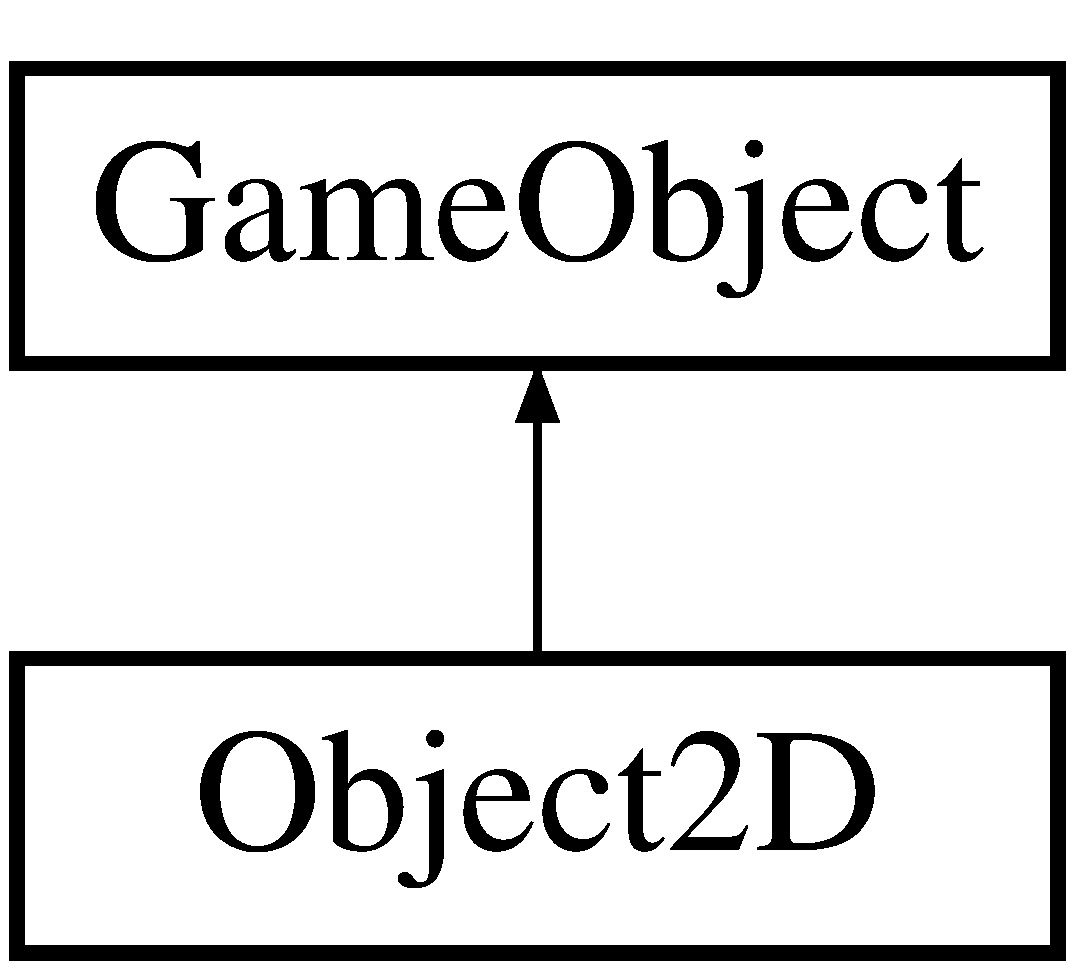
\includegraphics[height=2.000000cm]{class_object2_d}
\end{center}
\end{figure}
\subsection*{Public Member Functions}
\begin{DoxyCompactItemize}
\item 
\hyperlink{class_object2_d_adf886706d2a5aac31e1fbe0d71e8dc82}{Object2\-D} ()
\begin{DoxyCompactList}\small\item\em \mbox{[}brief description\mbox{]} \end{DoxyCompactList}\item 
int \hyperlink{class_object2_d_abeb56d59b3bd118d9ba5f098bae0c763}{is\-Type} ()
\begin{DoxyCompactList}\small\item\em \mbox{[}brief description\mbox{]} \end{DoxyCompactList}\item 
void \hyperlink{class_object2_d_a5a2f5ce24ca8a271932fbdb86bc8aa8e}{enable} (bool e)
\begin{DoxyCompactList}\small\item\em \mbox{[}brief description\mbox{]} \end{DoxyCompactList}\item 
bool \hyperlink{class_object2_d_a8a36288b9032a3ae53cac87e37c66716}{get\-Enable} ()
\begin{DoxyCompactList}\small\item\em \mbox{[}brief description\mbox{]} \end{DoxyCompactList}\item 
void \hyperlink{class_object2_d_a2d47915dce9714aecbc03038ff408df7}{translate} (float x, float y, float z)
\begin{DoxyCompactList}\small\item\em \mbox{[}brief description\mbox{]} \end{DoxyCompactList}\item 
void \hyperlink{class_object2_d_ab07a1bb40355a3f4c0a46357aa51a132}{set\-Pos} (float x, float y, float z)
\begin{DoxyCompactList}\small\item\em \mbox{[}brief description\mbox{]} \end{DoxyCompactList}\item 
\hyperlink{struct_vector3}{Vector3} \hyperlink{class_object2_d_a4d74800b53451bfa94d89f4dfba3d00a}{get\-Pos} ()
\begin{DoxyCompactList}\small\item\em \mbox{[}brief description\mbox{]} \end{DoxyCompactList}\item 
float \hyperlink{class_object2_d_a1e3b86ae9f6ab4c443ce12df0ef1730b}{get\-Pos\-X} ()
\begin{DoxyCompactList}\small\item\em \mbox{[}brief description\mbox{]} \end{DoxyCompactList}\item 
float \hyperlink{class_object2_d_a284eb150bf8c8ef6b383955302409a44}{get\-Pos\-Y} ()
\begin{DoxyCompactList}\small\item\em \mbox{[}brief description\mbox{]} \end{DoxyCompactList}\item 
float \hyperlink{class_object2_d_a8a72705600b30cb9594c21aa66b219a0}{get\-Pos\-Z} ()
\begin{DoxyCompactList}\small\item\em \mbox{[}brief description\mbox{]} \end{DoxyCompactList}\item 
void \hyperlink{class_object2_d_ae9379f6e64ee1d7661df355b91999d8d}{set\-Script} (const char $\ast$file)
\begin{DoxyCompactList}\small\item\em \mbox{[}brief description\mbox{]} \end{DoxyCompactList}\item 
std\-::string \hyperlink{class_object2_d_a953f9ebfc88c7d4ea4d155646c4f4a85}{get\-Script} ()
\begin{DoxyCompactList}\small\item\em \mbox{[}brief description\mbox{]} \end{DoxyCompactList}\item 
\hypertarget{class_object2_d_af39b3fe8563fa2b99ecbcfb5af89cd92}{std\-::string {\bfseries get\-Name} ()}\label{class_object2_d_af39b3fe8563fa2b99ecbcfb5af89cd92}

\item 
\hypertarget{class_object2_d_ac0b12924c5939c854efc213c1367aecb}{void {\bfseries set\-Name} (std\-::string n)}\label{class_object2_d_ac0b12924c5939c854efc213c1367aecb}

\item 
\hypertarget{class_object2_d_a7c0928456483dec69466938f2277f371}{std\-::string {\bfseries get\-Texture} ()}\label{class_object2_d_a7c0928456483dec69466938f2277f371}

\item 
\hypertarget{class_object2_d_ac202a1df015571805ac6432a574d8c29}{void {\bfseries set\-Texture} (std\-::string t)}\label{class_object2_d_ac202a1df015571805ac6432a574d8c29}

\item 
\hypertarget{class_object2_d_a296217271f737141b4cda09c1347a8b0}{float {\bfseries get\-Translate\-X} ()}\label{class_object2_d_a296217271f737141b4cda09c1347a8b0}

\item 
\hypertarget{class_object2_d_a7269f877b6ba784bd982e145b3cde40a}{float {\bfseries get\-Translate\-Y} ()}\label{class_object2_d_a7269f877b6ba784bd982e145b3cde40a}

\item 
\hypertarget{class_object2_d_a80e3245c977d904af2e60d5321e57d58}{float {\bfseries get\-Translate\-Z} ()}\label{class_object2_d_a80e3245c977d904af2e60d5321e57d58}

\item 
\hypertarget{class_object2_d_acaac60e76eb6bca23216293961cede8e}{void {\bfseries set\-Rotation} (Axis axis, float angle)}\label{class_object2_d_acaac60e76eb6bca23216293961cede8e}

\item 
\hypertarget{class_object2_d_ab3a5b9b3570efb91a7ba248015b90ef3}{float {\bfseries get\-Rotation\-X} ()}\label{class_object2_d_ab3a5b9b3570efb91a7ba248015b90ef3}

\item 
\hypertarget{class_object2_d_a357e962fc8e9920c1710e33813b2867e}{float {\bfseries get\-Rotation\-Y} ()}\label{class_object2_d_a357e962fc8e9920c1710e33813b2867e}

\item 
\hypertarget{class_object2_d_a1e8e73a4ac5183df5766c23f77288b9a}{float {\bfseries get\-Rotation\-Z} ()}\label{class_object2_d_a1e8e73a4ac5183df5766c23f77288b9a}

\end{DoxyCompactItemize}
\subsection*{Additional Inherited Members}


\subsection{Detailed Description}
\mbox{[}brief description\mbox{]} 

\mbox{[}long description\mbox{]} \begin{DoxyReturn}{Returns}
\mbox{[}description\mbox{]} 
\end{DoxyReturn}


\subsection{Constructor \& Destructor Documentation}
\hypertarget{class_object2_d_adf886706d2a5aac31e1fbe0d71e8dc82}{\index{Object2\-D@{Object2\-D}!Object2\-D@{Object2\-D}}
\index{Object2\-D@{Object2\-D}!Object2D@{Object2\-D}}
\subsubsection[{Object2\-D}]{\setlength{\rightskip}{0pt plus 5cm}Object2\-D\-::\-Object2\-D (
\begin{DoxyParamCaption}
{}
\end{DoxyParamCaption}
)}}\label{class_object2_d_adf886706d2a5aac31e1fbe0d71e8dc82}


\mbox{[}brief description\mbox{]} 

\mbox{[}long description\mbox{]} 

\subsection{Member Function Documentation}
\hypertarget{class_object2_d_a5a2f5ce24ca8a271932fbdb86bc8aa8e}{\index{Object2\-D@{Object2\-D}!enable@{enable}}
\index{enable@{enable}!Object2D@{Object2\-D}}
\subsubsection[{enable}]{\setlength{\rightskip}{0pt plus 5cm}void Object2\-D\-::enable (
\begin{DoxyParamCaption}
\item[{bool}]{e}
\end{DoxyParamCaption}
)\hspace{0.3cm}{\ttfamily [virtual]}}}\label{class_object2_d_a5a2f5ce24ca8a271932fbdb86bc8aa8e}


\mbox{[}brief description\mbox{]} 

\mbox{[}long description\mbox{]}


\begin{DoxyParams}{Parameters}
{\em m} & \mbox{[}description\mbox{]} \\
\hline
{\em t} & \mbox{[}description\mbox{]} \\
\hline
\end{DoxyParams}


Implements \hyperlink{class_game_object_a5e7b5056ab92f998cda8fa3779bf44d1}{Game\-Object}.

\hypertarget{class_object2_d_a8a36288b9032a3ae53cac87e37c66716}{\index{Object2\-D@{Object2\-D}!get\-Enable@{get\-Enable}}
\index{get\-Enable@{get\-Enable}!Object2D@{Object2\-D}}
\subsubsection[{get\-Enable}]{\setlength{\rightskip}{0pt plus 5cm}bool Object2\-D\-::get\-Enable (
\begin{DoxyParamCaption}
{}
\end{DoxyParamCaption}
)\hspace{0.3cm}{\ttfamily [virtual]}}}\label{class_object2_d_a8a36288b9032a3ae53cac87e37c66716}


\mbox{[}brief description\mbox{]} 

\mbox{[}long description\mbox{]}


\begin{DoxyParams}{Parameters}
{\em m} & \mbox{[}description\mbox{]} \\
\hline
{\em t} & \mbox{[}description\mbox{]} \\
\hline
\end{DoxyParams}


Implements \hyperlink{class_game_object_a0fa51b1d4bcf6756e4a5e1637fa01d78}{Game\-Object}.

\hypertarget{class_object2_d_a4d74800b53451bfa94d89f4dfba3d00a}{\index{Object2\-D@{Object2\-D}!get\-Pos@{get\-Pos}}
\index{get\-Pos@{get\-Pos}!Object2D@{Object2\-D}}
\subsubsection[{get\-Pos}]{\setlength{\rightskip}{0pt plus 5cm}{\bf Vector3} Object2\-D\-::get\-Pos (
\begin{DoxyParamCaption}
{}
\end{DoxyParamCaption}
)\hspace{0.3cm}{\ttfamily [virtual]}}}\label{class_object2_d_a4d74800b53451bfa94d89f4dfba3d00a}


\mbox{[}brief description\mbox{]} 

\mbox{[}long description\mbox{]} \begin{DoxyReturn}{Returns}
\mbox{[}description\mbox{]} 
\end{DoxyReturn}


Implements \hyperlink{class_game_object_a01903e73800537f21d25040de96b1e0a}{Game\-Object}.

\hypertarget{class_object2_d_a1e3b86ae9f6ab4c443ce12df0ef1730b}{\index{Object2\-D@{Object2\-D}!get\-Pos\-X@{get\-Pos\-X}}
\index{get\-Pos\-X@{get\-Pos\-X}!Object2D@{Object2\-D}}
\subsubsection[{get\-Pos\-X}]{\setlength{\rightskip}{0pt plus 5cm}float Object2\-D\-::get\-Pos\-X (
\begin{DoxyParamCaption}
{}
\end{DoxyParamCaption}
)\hspace{0.3cm}{\ttfamily [virtual]}}}\label{class_object2_d_a1e3b86ae9f6ab4c443ce12df0ef1730b}


\mbox{[}brief description\mbox{]} 

\mbox{[}long description\mbox{]} \begin{DoxyReturn}{Returns}
\mbox{[}description\mbox{]} 
\end{DoxyReturn}


Implements \hyperlink{class_game_object_ab41e4a13b4e37f7a40a9e5cf54db07d9}{Game\-Object}.

\hypertarget{class_object2_d_a284eb150bf8c8ef6b383955302409a44}{\index{Object2\-D@{Object2\-D}!get\-Pos\-Y@{get\-Pos\-Y}}
\index{get\-Pos\-Y@{get\-Pos\-Y}!Object2D@{Object2\-D}}
\subsubsection[{get\-Pos\-Y}]{\setlength{\rightskip}{0pt plus 5cm}float Object2\-D\-::get\-Pos\-Y (
\begin{DoxyParamCaption}
{}
\end{DoxyParamCaption}
)\hspace{0.3cm}{\ttfamily [virtual]}}}\label{class_object2_d_a284eb150bf8c8ef6b383955302409a44}


\mbox{[}brief description\mbox{]} 

\mbox{[}long description\mbox{]} \begin{DoxyReturn}{Returns}
\mbox{[}description\mbox{]} 
\end{DoxyReturn}


Implements \hyperlink{class_game_object_aab59caeb6b903c23a76be1ddb1497a60}{Game\-Object}.

\hypertarget{class_object2_d_a8a72705600b30cb9594c21aa66b219a0}{\index{Object2\-D@{Object2\-D}!get\-Pos\-Z@{get\-Pos\-Z}}
\index{get\-Pos\-Z@{get\-Pos\-Z}!Object2D@{Object2\-D}}
\subsubsection[{get\-Pos\-Z}]{\setlength{\rightskip}{0pt plus 5cm}float Object2\-D\-::get\-Pos\-Z (
\begin{DoxyParamCaption}
{}
\end{DoxyParamCaption}
)\hspace{0.3cm}{\ttfamily [virtual]}}}\label{class_object2_d_a8a72705600b30cb9594c21aa66b219a0}


\mbox{[}brief description\mbox{]} 

\mbox{[}long description\mbox{]} \begin{DoxyReturn}{Returns}
\mbox{[}description\mbox{]} 
\end{DoxyReturn}


Implements \hyperlink{class_game_object_a0eb3185aa4070664b4b7a6f23ae64f32}{Game\-Object}.

\hypertarget{class_object2_d_a953f9ebfc88c7d4ea4d155646c4f4a85}{\index{Object2\-D@{Object2\-D}!get\-Script@{get\-Script}}
\index{get\-Script@{get\-Script}!Object2D@{Object2\-D}}
\subsubsection[{get\-Script}]{\setlength{\rightskip}{0pt plus 5cm}std\-::string Object2\-D\-::get\-Script (
\begin{DoxyParamCaption}
{}
\end{DoxyParamCaption}
)\hspace{0.3cm}{\ttfamily [virtual]}}}\label{class_object2_d_a953f9ebfc88c7d4ea4d155646c4f4a85}


\mbox{[}brief description\mbox{]} 

\mbox{[}long description\mbox{]} \begin{DoxyReturn}{Returns}
\mbox{[}description\mbox{]} 
\end{DoxyReturn}


Implements \hyperlink{class_game_object_af8c16297dbff83e1ae7c4f75f314b856}{Game\-Object}.

\hypertarget{class_object2_d_abeb56d59b3bd118d9ba5f098bae0c763}{\index{Object2\-D@{Object2\-D}!is\-Type@{is\-Type}}
\index{is\-Type@{is\-Type}!Object2D@{Object2\-D}}
\subsubsection[{is\-Type}]{\setlength{\rightskip}{0pt plus 5cm}int Object2\-D\-::is\-Type (
\begin{DoxyParamCaption}
{}
\end{DoxyParamCaption}
)\hspace{0.3cm}{\ttfamily [virtual]}}}\label{class_object2_d_abeb56d59b3bd118d9ba5f098bae0c763}


\mbox{[}brief description\mbox{]} 

\mbox{[}long description\mbox{]} \begin{DoxyReturn}{Returns}
\mbox{[}description\mbox{]} 
\end{DoxyReturn}


Implements \hyperlink{class_game_object_a1d4237f8e511d5c6f0b1ad92480199b3}{Game\-Object}.

\hypertarget{class_object2_d_ab07a1bb40355a3f4c0a46357aa51a132}{\index{Object2\-D@{Object2\-D}!set\-Pos@{set\-Pos}}
\index{set\-Pos@{set\-Pos}!Object2D@{Object2\-D}}
\subsubsection[{set\-Pos}]{\setlength{\rightskip}{0pt plus 5cm}void Object2\-D\-::set\-Pos (
\begin{DoxyParamCaption}
\item[{float}]{x, }
\item[{float}]{y, }
\item[{float}]{z}
\end{DoxyParamCaption}
)\hspace{0.3cm}{\ttfamily [virtual]}}}\label{class_object2_d_ab07a1bb40355a3f4c0a46357aa51a132}


\mbox{[}brief description\mbox{]} 

\mbox{[}long description\mbox{]}


\begin{DoxyParams}{Parameters}
{\em x} & \mbox{[}description\mbox{]} \\
\hline
{\em y} & \mbox{[}description\mbox{]} \\
\hline
{\em z} & \mbox{[}description\mbox{]} \\
\hline
\end{DoxyParams}


Implements \hyperlink{class_game_object_a6f33cf0e915855f22c7e115625138567}{Game\-Object}.

\hypertarget{class_object2_d_ae9379f6e64ee1d7661df355b91999d8d}{\index{Object2\-D@{Object2\-D}!set\-Script@{set\-Script}}
\index{set\-Script@{set\-Script}!Object2D@{Object2\-D}}
\subsubsection[{set\-Script}]{\setlength{\rightskip}{0pt plus 5cm}void Object2\-D\-::set\-Script (
\begin{DoxyParamCaption}
\item[{const char $\ast$}]{file}
\end{DoxyParamCaption}
)\hspace{0.3cm}{\ttfamily [virtual]}}}\label{class_object2_d_ae9379f6e64ee1d7661df355b91999d8d}


\mbox{[}brief description\mbox{]} 

\mbox{[}long description\mbox{]}


\begin{DoxyParams}{Parameters}
{\em file} & \mbox{[}description\mbox{]} \\
\hline
\end{DoxyParams}


Implements \hyperlink{class_game_object_a3cdd9cb174d5fa4d4a5748df1ab09e87}{Game\-Object}.

\hypertarget{class_object2_d_a2d47915dce9714aecbc03038ff408df7}{\index{Object2\-D@{Object2\-D}!translate@{translate}}
\index{translate@{translate}!Object2D@{Object2\-D}}
\subsubsection[{translate}]{\setlength{\rightskip}{0pt plus 5cm}void Object2\-D\-::translate (
\begin{DoxyParamCaption}
\item[{float}]{x, }
\item[{float}]{y, }
\item[{float}]{z}
\end{DoxyParamCaption}
)\hspace{0.3cm}{\ttfamily [virtual]}}}\label{class_object2_d_a2d47915dce9714aecbc03038ff408df7}


\mbox{[}brief description\mbox{]} 

\mbox{[}long description\mbox{]}


\begin{DoxyParams}{Parameters}
{\em x} & \mbox{[}description\mbox{]} \\
\hline
{\em y} & \mbox{[}description\mbox{]} \\
\hline
{\em z} & \mbox{[}description\mbox{]} \\
\hline
\end{DoxyParams}


Implements \hyperlink{class_game_object_a00ebf6691d90a55af08dd1b1afd7abaf}{Game\-Object}.



The documentation for this class was generated from the following files\-:\begin{DoxyCompactItemize}
\item 
E\-:/\-G\-R\-A\-B\-L\-A\-U\-R\-G/\-I\-S\-E/\-I\-S\-E-\/\-Demo/\-I\-S\-E-\/\-Demo/Game\-Object.\-h\item 
E\-:/\-G\-R\-A\-B\-L\-A\-U\-R\-G/\-I\-S\-E/\-I\-S\-E-\/\-Demo/\-I\-S\-E-\/\-Demo/Object2\-D.\-cpp\end{DoxyCompactItemize}

\hypertarget{class_object3_d}{\section{Object3\-D Class Reference}
\label{class_object3_d}\index{Object3\-D@{Object3\-D}}
}


\mbox{[}brief description\mbox{]}  




{\ttfamily \#include $<$Game\-Object.\-h$>$}

Inheritance diagram for Object3\-D\-:\begin{figure}[H]
\begin{center}
\leavevmode
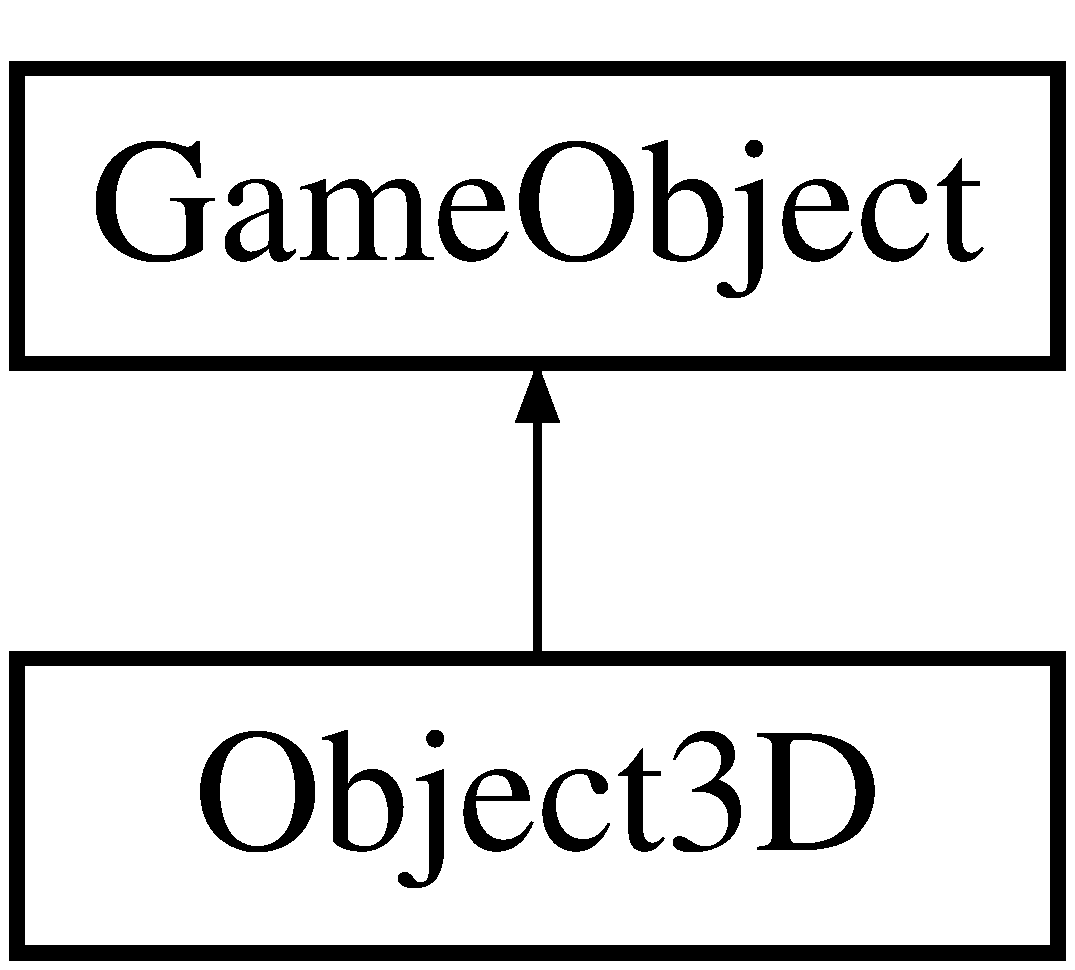
\includegraphics[height=2.000000cm]{class_object3_d}
\end{center}
\end{figure}
\subsection*{Public Member Functions}
\begin{DoxyCompactItemize}
\item 
\hyperlink{class_object3_d_ae3a1b17fb43ab59f5cf7b0ee21b9120b}{Object3\-D} ()
\begin{DoxyCompactList}\small\item\em \mbox{[}brief description\mbox{]} \end{DoxyCompactList}\item 
int \hyperlink{class_object3_d_af9a973bc07b6dcdacefebe20023a1d51}{is\-Type} ()
\begin{DoxyCompactList}\small\item\em \mbox{[}brief description\mbox{]} \end{DoxyCompactList}\item 
void \hyperlink{class_object3_d_a83b58f2bd94df5fb41cdd2ad2718b738}{enable} (bool enable)
\begin{DoxyCompactList}\small\item\em \mbox{[}brief description\mbox{]} \end{DoxyCompactList}\item 
bool \hyperlink{class_object3_d_ac51d638d70d1200d44d468945bfc0356}{get\-Enable} ()
\begin{DoxyCompactList}\small\item\em \mbox{[}brief description\mbox{]} \end{DoxyCompactList}\item 
void \hyperlink{class_object3_d_a1362e9e4752b6ce4bddb1fa69e0e0894}{translate} (float x, float y, float z)
\begin{DoxyCompactList}\small\item\em \mbox{[}brief description\mbox{]} \end{DoxyCompactList}\item 
void \hyperlink{class_object3_d_a4913643d7f24106e2272e3cf6c49bb8e}{set\-Pos} (float x, float y, float z)
\begin{DoxyCompactList}\small\item\em \mbox{[}brief description\mbox{]} \end{DoxyCompactList}\item 
\hyperlink{struct_vector3}{Vector3} \hyperlink{class_object3_d_a7c4949df5017e162cd5921ed18061730}{get\-Pos} ()
\begin{DoxyCompactList}\small\item\em \mbox{[}brief description\mbox{]} \end{DoxyCompactList}\item 
float \hyperlink{class_object3_d_a76e35761a85a8660b078a3a4780c2525}{get\-Pos\-X} ()
\begin{DoxyCompactList}\small\item\em \mbox{[}brief description\mbox{]} \end{DoxyCompactList}\item 
float \hyperlink{class_object3_d_a960a658a0c324bb13f5c230a52dabed9}{get\-Pos\-Y} ()
\begin{DoxyCompactList}\small\item\em \mbox{[}brief description\mbox{]} \end{DoxyCompactList}\item 
float \hyperlink{class_object3_d_a065ea3924cb5d9ba4fa70e2226d74e8d}{get\-Pos\-Z} ()
\begin{DoxyCompactList}\small\item\em \mbox{[}brief description\mbox{]} \end{DoxyCompactList}\item 
void \hyperlink{class_object3_d_a2f0bffd2963d34f7496531f35cfcb5ef}{set\-Script} (const char $\ast$file)
\begin{DoxyCompactList}\small\item\em \mbox{[}brief description\mbox{]} \end{DoxyCompactList}\item 
std\-::string \hyperlink{class_object3_d_a9e3a956e808621d37029941057724fab}{get\-Script} ()
\begin{DoxyCompactList}\small\item\em \mbox{[}brief description\mbox{]} \end{DoxyCompactList}\item 
\hypertarget{class_object3_d_aa80515b56146b062e55d91c01cbbba02}{std\-::string {\bfseries get\-Name} ()}\label{class_object3_d_aa80515b56146b062e55d91c01cbbba02}

\item 
\hypertarget{class_object3_d_af290d9de7127fda74883ae224baa88d6}{void {\bfseries set\-Name} (std\-::string n)}\label{class_object3_d_af290d9de7127fda74883ae224baa88d6}

\item 
\hypertarget{class_object3_d_a352441fd7f71023368e84b5b4f4387a4}{std\-::string {\bfseries get\-Texture} ()}\label{class_object3_d_a352441fd7f71023368e84b5b4f4387a4}

\item 
\hypertarget{class_object3_d_a2dbe7dd0df57b2eb770476c0878e5d2d}{void {\bfseries set\-Texture} (std\-::string t)}\label{class_object3_d_a2dbe7dd0df57b2eb770476c0878e5d2d}

\item 
\hypertarget{class_object3_d_af732ce29402725c98242f9672f615785}{float {\bfseries get\-Translate\-X} ()}\label{class_object3_d_af732ce29402725c98242f9672f615785}

\item 
\hypertarget{class_object3_d_ac8a7975a62006b86519e3089858a089d}{float {\bfseries get\-Translate\-Y} ()}\label{class_object3_d_ac8a7975a62006b86519e3089858a089d}

\item 
\hypertarget{class_object3_d_a95cdfa73ea33fb5c7770fa17a3b0ba4f}{float {\bfseries get\-Translate\-Z} ()}\label{class_object3_d_a95cdfa73ea33fb5c7770fa17a3b0ba4f}

\item 
\hypertarget{class_object3_d_a9e27b2de1331860441b0d44d9af8f59c}{void {\bfseries set\-Rotation} (Axis axis, float angle)}\label{class_object3_d_a9e27b2de1331860441b0d44d9af8f59c}

\item 
\hypertarget{class_object3_d_a468416e177fc4fd035b3ab9f36e2e31b}{float {\bfseries get\-Rotation\-X} ()}\label{class_object3_d_a468416e177fc4fd035b3ab9f36e2e31b}

\item 
\hypertarget{class_object3_d_a5e4b0659327d83244b8fdf7d68880635}{float {\bfseries get\-Rotation\-Y} ()}\label{class_object3_d_a5e4b0659327d83244b8fdf7d68880635}

\item 
\hypertarget{class_object3_d_aa84c252e5ae73542b3df96b17b270b58}{float {\bfseries get\-Rotation\-Z} ()}\label{class_object3_d_aa84c252e5ae73542b3df96b17b270b58}

\end{DoxyCompactItemize}
\subsection*{Additional Inherited Members}


\subsection{Detailed Description}
\mbox{[}brief description\mbox{]} 

\mbox{[}long description\mbox{]} \begin{DoxyReturn}{Returns}
\mbox{[}description\mbox{]} 
\end{DoxyReturn}
\begin{DoxyAuthor}{Author}
\mbox{[}author\mbox{]} 
\end{DoxyAuthor}


\subsection{Constructor \& Destructor Documentation}
\hypertarget{class_object3_d_ae3a1b17fb43ab59f5cf7b0ee21b9120b}{\index{Object3\-D@{Object3\-D}!Object3\-D@{Object3\-D}}
\index{Object3\-D@{Object3\-D}!Object3D@{Object3\-D}}
\subsubsection[{Object3\-D}]{\setlength{\rightskip}{0pt plus 5cm}Object3\-D\-::\-Object3\-D (
\begin{DoxyParamCaption}
{}
\end{DoxyParamCaption}
)}}\label{class_object3_d_ae3a1b17fb43ab59f5cf7b0ee21b9120b}


\mbox{[}brief description\mbox{]} 

\mbox{[}long description\mbox{]} 

\subsection{Member Function Documentation}
\hypertarget{class_object3_d_a83b58f2bd94df5fb41cdd2ad2718b738}{\index{Object3\-D@{Object3\-D}!enable@{enable}}
\index{enable@{enable}!Object3D@{Object3\-D}}
\subsubsection[{enable}]{\setlength{\rightskip}{0pt plus 5cm}void Object3\-D\-::enable (
\begin{DoxyParamCaption}
\item[{bool}]{enable}
\end{DoxyParamCaption}
)\hspace{0.3cm}{\ttfamily [virtual]}}}\label{class_object3_d_a83b58f2bd94df5fb41cdd2ad2718b738}


\mbox{[}brief description\mbox{]} 

\mbox{[}long description\mbox{]}


\begin{DoxyParams}{Parameters}
{\em m} & \mbox{[}description\mbox{]} \\
\hline
{\em t} & \mbox{[}description\mbox{]} \\
\hline
\end{DoxyParams}


Implements \hyperlink{class_game_object_a5e7b5056ab92f998cda8fa3779bf44d1}{Game\-Object}.

\hypertarget{class_object3_d_ac51d638d70d1200d44d468945bfc0356}{\index{Object3\-D@{Object3\-D}!get\-Enable@{get\-Enable}}
\index{get\-Enable@{get\-Enable}!Object3D@{Object3\-D}}
\subsubsection[{get\-Enable}]{\setlength{\rightskip}{0pt plus 5cm}bool Object3\-D\-::get\-Enable (
\begin{DoxyParamCaption}
{}
\end{DoxyParamCaption}
)\hspace{0.3cm}{\ttfamily [virtual]}}}\label{class_object3_d_ac51d638d70d1200d44d468945bfc0356}


\mbox{[}brief description\mbox{]} 

\mbox{[}long description\mbox{]}


\begin{DoxyParams}{Parameters}
{\em m} & \mbox{[}description\mbox{]} \\
\hline
{\em t} & \mbox{[}description\mbox{]} \\
\hline
\end{DoxyParams}


Implements \hyperlink{class_game_object_a0fa51b1d4bcf6756e4a5e1637fa01d78}{Game\-Object}.

\hypertarget{class_object3_d_a7c4949df5017e162cd5921ed18061730}{\index{Object3\-D@{Object3\-D}!get\-Pos@{get\-Pos}}
\index{get\-Pos@{get\-Pos}!Object3D@{Object3\-D}}
\subsubsection[{get\-Pos}]{\setlength{\rightskip}{0pt plus 5cm}{\bf Vector3} Object3\-D\-::get\-Pos (
\begin{DoxyParamCaption}
{}
\end{DoxyParamCaption}
)\hspace{0.3cm}{\ttfamily [virtual]}}}\label{class_object3_d_a7c4949df5017e162cd5921ed18061730}


\mbox{[}brief description\mbox{]} 

\mbox{[}long description\mbox{]} \begin{DoxyReturn}{Returns}
\mbox{[}description\mbox{]} 
\end{DoxyReturn}


Implements \hyperlink{class_game_object_a01903e73800537f21d25040de96b1e0a}{Game\-Object}.

\hypertarget{class_object3_d_a76e35761a85a8660b078a3a4780c2525}{\index{Object3\-D@{Object3\-D}!get\-Pos\-X@{get\-Pos\-X}}
\index{get\-Pos\-X@{get\-Pos\-X}!Object3D@{Object3\-D}}
\subsubsection[{get\-Pos\-X}]{\setlength{\rightskip}{0pt plus 5cm}float Object3\-D\-::get\-Pos\-X (
\begin{DoxyParamCaption}
{}
\end{DoxyParamCaption}
)\hspace{0.3cm}{\ttfamily [virtual]}}}\label{class_object3_d_a76e35761a85a8660b078a3a4780c2525}


\mbox{[}brief description\mbox{]} 

\mbox{[}long description\mbox{]} \begin{DoxyReturn}{Returns}
\mbox{[}description\mbox{]} 
\end{DoxyReturn}


Implements \hyperlink{class_game_object_ab41e4a13b4e37f7a40a9e5cf54db07d9}{Game\-Object}.

\hypertarget{class_object3_d_a960a658a0c324bb13f5c230a52dabed9}{\index{Object3\-D@{Object3\-D}!get\-Pos\-Y@{get\-Pos\-Y}}
\index{get\-Pos\-Y@{get\-Pos\-Y}!Object3D@{Object3\-D}}
\subsubsection[{get\-Pos\-Y}]{\setlength{\rightskip}{0pt plus 5cm}float Object3\-D\-::get\-Pos\-Y (
\begin{DoxyParamCaption}
{}
\end{DoxyParamCaption}
)\hspace{0.3cm}{\ttfamily [virtual]}}}\label{class_object3_d_a960a658a0c324bb13f5c230a52dabed9}


\mbox{[}brief description\mbox{]} 

\mbox{[}long description\mbox{]} \begin{DoxyReturn}{Returns}
\mbox{[}description\mbox{]} 
\end{DoxyReturn}


Implements \hyperlink{class_game_object_aab59caeb6b903c23a76be1ddb1497a60}{Game\-Object}.

\hypertarget{class_object3_d_a065ea3924cb5d9ba4fa70e2226d74e8d}{\index{Object3\-D@{Object3\-D}!get\-Pos\-Z@{get\-Pos\-Z}}
\index{get\-Pos\-Z@{get\-Pos\-Z}!Object3D@{Object3\-D}}
\subsubsection[{get\-Pos\-Z}]{\setlength{\rightskip}{0pt plus 5cm}float Object3\-D\-::get\-Pos\-Z (
\begin{DoxyParamCaption}
{}
\end{DoxyParamCaption}
)\hspace{0.3cm}{\ttfamily [virtual]}}}\label{class_object3_d_a065ea3924cb5d9ba4fa70e2226d74e8d}


\mbox{[}brief description\mbox{]} 

\mbox{[}long description\mbox{]} \begin{DoxyReturn}{Returns}
\mbox{[}description\mbox{]} 
\end{DoxyReturn}


Implements \hyperlink{class_game_object_a0eb3185aa4070664b4b7a6f23ae64f32}{Game\-Object}.

\hypertarget{class_object3_d_a9e3a956e808621d37029941057724fab}{\index{Object3\-D@{Object3\-D}!get\-Script@{get\-Script}}
\index{get\-Script@{get\-Script}!Object3D@{Object3\-D}}
\subsubsection[{get\-Script}]{\setlength{\rightskip}{0pt plus 5cm}std\-::string Object3\-D\-::get\-Script (
\begin{DoxyParamCaption}
{}
\end{DoxyParamCaption}
)\hspace{0.3cm}{\ttfamily [virtual]}}}\label{class_object3_d_a9e3a956e808621d37029941057724fab}


\mbox{[}brief description\mbox{]} 

\mbox{[}long description\mbox{]} \begin{DoxyReturn}{Returns}
\mbox{[}description\mbox{]} 
\end{DoxyReturn}


Implements \hyperlink{class_game_object_af8c16297dbff83e1ae7c4f75f314b856}{Game\-Object}.

\hypertarget{class_object3_d_af9a973bc07b6dcdacefebe20023a1d51}{\index{Object3\-D@{Object3\-D}!is\-Type@{is\-Type}}
\index{is\-Type@{is\-Type}!Object3D@{Object3\-D}}
\subsubsection[{is\-Type}]{\setlength{\rightskip}{0pt plus 5cm}int Object3\-D\-::is\-Type (
\begin{DoxyParamCaption}
{}
\end{DoxyParamCaption}
)\hspace{0.3cm}{\ttfamily [virtual]}}}\label{class_object3_d_af9a973bc07b6dcdacefebe20023a1d51}


\mbox{[}brief description\mbox{]} 

\mbox{[}long description\mbox{]} \begin{DoxyReturn}{Returns}
\mbox{[}description\mbox{]} 
\end{DoxyReturn}


Implements \hyperlink{class_game_object_a1d4237f8e511d5c6f0b1ad92480199b3}{Game\-Object}.

\hypertarget{class_object3_d_a4913643d7f24106e2272e3cf6c49bb8e}{\index{Object3\-D@{Object3\-D}!set\-Pos@{set\-Pos}}
\index{set\-Pos@{set\-Pos}!Object3D@{Object3\-D}}
\subsubsection[{set\-Pos}]{\setlength{\rightskip}{0pt plus 5cm}void Object3\-D\-::set\-Pos (
\begin{DoxyParamCaption}
\item[{float}]{x, }
\item[{float}]{y, }
\item[{float}]{z}
\end{DoxyParamCaption}
)\hspace{0.3cm}{\ttfamily [virtual]}}}\label{class_object3_d_a4913643d7f24106e2272e3cf6c49bb8e}


\mbox{[}brief description\mbox{]} 

\mbox{[}long description\mbox{]}


\begin{DoxyParams}{Parameters}
{\em x} & \mbox{[}description\mbox{]} \\
\hline
{\em y} & \mbox{[}description\mbox{]} \\
\hline
{\em z} & \mbox{[}description\mbox{]} \\
\hline
\end{DoxyParams}


Implements \hyperlink{class_game_object_a6f33cf0e915855f22c7e115625138567}{Game\-Object}.

\hypertarget{class_object3_d_a2f0bffd2963d34f7496531f35cfcb5ef}{\index{Object3\-D@{Object3\-D}!set\-Script@{set\-Script}}
\index{set\-Script@{set\-Script}!Object3D@{Object3\-D}}
\subsubsection[{set\-Script}]{\setlength{\rightskip}{0pt plus 5cm}void Object3\-D\-::set\-Script (
\begin{DoxyParamCaption}
\item[{const char $\ast$}]{file}
\end{DoxyParamCaption}
)\hspace{0.3cm}{\ttfamily [virtual]}}}\label{class_object3_d_a2f0bffd2963d34f7496531f35cfcb5ef}


\mbox{[}brief description\mbox{]} 

\mbox{[}long description\mbox{]}


\begin{DoxyParams}{Parameters}
{\em file} & \mbox{[}description\mbox{]} \\
\hline
\end{DoxyParams}


Implements \hyperlink{class_game_object_a3cdd9cb174d5fa4d4a5748df1ab09e87}{Game\-Object}.

\hypertarget{class_object3_d_a1362e9e4752b6ce4bddb1fa69e0e0894}{\index{Object3\-D@{Object3\-D}!translate@{translate}}
\index{translate@{translate}!Object3D@{Object3\-D}}
\subsubsection[{translate}]{\setlength{\rightskip}{0pt plus 5cm}void Object3\-D\-::translate (
\begin{DoxyParamCaption}
\item[{float}]{x, }
\item[{float}]{y, }
\item[{float}]{z}
\end{DoxyParamCaption}
)\hspace{0.3cm}{\ttfamily [virtual]}}}\label{class_object3_d_a1362e9e4752b6ce4bddb1fa69e0e0894}


\mbox{[}brief description\mbox{]} 

\mbox{[}long description\mbox{]}


\begin{DoxyParams}{Parameters}
{\em x} & \mbox{[}description\mbox{]} \\
\hline
{\em y} & \mbox{[}description\mbox{]} \\
\hline
{\em z} & \mbox{[}description\mbox{]} \\
\hline
\end{DoxyParams}


Implements \hyperlink{class_game_object_a00ebf6691d90a55af08dd1b1afd7abaf}{Game\-Object}.



The documentation for this class was generated from the following files\-:\begin{DoxyCompactItemize}
\item 
E\-:/\-G\-R\-A\-B\-L\-A\-U\-R\-G/\-I\-S\-E/\-I\-S\-E-\/\-Demo/\-I\-S\-E-\/\-Demo/Game\-Object.\-h\item 
E\-:/\-G\-R\-A\-B\-L\-A\-U\-R\-G/\-I\-S\-E/\-I\-S\-E-\/\-Demo/\-I\-S\-E-\/\-Demo/Object3\-D.\-cpp\end{DoxyCompactItemize}

\hypertarget{classobj_loader}{\section{obj\-Loader Class Reference}
\label{classobj_loader}\index{obj\-Loader@{obj\-Loader}}
}


A Loader function that converts the model data into the common \hyperlink{class_v_a_o}{V\-A\-O} format.  




{\ttfamily \#include $<$obj\-Loader.\-h$>$}

\subsection*{Static Public Member Functions}
\begin{DoxyCompactItemize}
\item 
static \hyperlink{class_v_a_o}{V\-A\-O} \hyperlink{classobj_loader_a203279b541b0b95974d6aed84ec686aa}{load} (std\-::string location)
\begin{DoxyCompactList}\small\item\em load data from model \end{DoxyCompactList}\end{DoxyCompactItemize}


\subsection{Detailed Description}
A Loader function that converts the model data into the common \hyperlink{class_v_a_o}{V\-A\-O} format. 

\begin{DoxyReturn}{Returns}
\hyperlink{class_v_a_o}{V\-A\-O}, containing the model data needed to be drawn in opengl 
\end{DoxyReturn}
\begin{DoxyAuthor}{Author}
Umar Badat 
\end{DoxyAuthor}
\begin{DoxyNote}{Note}
I would like to expand the data loaded in to allow it to get more information about the models 
\end{DoxyNote}


\subsection{Member Function Documentation}
\hypertarget{classobj_loader_a203279b541b0b95974d6aed84ec686aa}{\index{obj\-Loader@{obj\-Loader}!load@{load}}
\index{load@{load}!objLoader@{obj\-Loader}}
\subsubsection[{load}]{\setlength{\rightskip}{0pt plus 5cm}{\bf V\-A\-O} obj\-Loader\-::load (
\begin{DoxyParamCaption}
\item[{std\-::string}]{location}
\end{DoxyParamCaption}
)\hspace{0.3cm}{\ttfamily [static]}}}\label{classobj_loader_a203279b541b0b95974d6aed84ec686aa}


load data from model 

Loads data from a range of model formats and coverts them to \hyperlink{class_v_a_o}{V\-A\-O}'s so the render engine only needs to handle one type


\begin{DoxyParams}{Parameters}
{\em location} & The name and location of the file you want to load in. \\
\hline
\end{DoxyParams}
\begin{DoxyReturn}{Returns}
\hyperlink{class_v_a_o}{V\-A\-O}, containing all the data. 
\end{DoxyReturn}


The documentation for this class was generated from the following files\-:\begin{DoxyCompactItemize}
\item 
E\-:/\-G\-R\-A\-B\-L\-A\-U\-R\-G/\-I\-S\-E/\-I\-S\-E-\/\-Demo/\-I\-S\-E-\/\-Demo/obj\-Loader.\-h\item 
E\-:/\-G\-R\-A\-B\-L\-A\-U\-R\-G/\-I\-S\-E/\-I\-S\-E-\/\-Demo/\-I\-S\-E-\/\-Demo/obj\-Loader.\-cpp\end{DoxyCompactItemize}

\hypertarget{class_o_p_e_n_g_l___facade}{\section{O\-P\-E\-N\-G\-L\-\_\-\-Facade Class Reference}
\label{class_o_p_e_n_g_l___facade}\index{O\-P\-E\-N\-G\-L\-\_\-\-Facade@{O\-P\-E\-N\-G\-L\-\_\-\-Facade}}
}
\subsection*{Static Public Member Functions}
\begin{DoxyCompactItemize}
\item 
static bool \hyperlink{class_o_p_e_n_g_l___facade_ae0412d4df1d7ff1120503166033779ef}{colour} (float R, float G, float B)
\begin{DoxyCompactList}\small\item\em Specifies the Color you write to when you clear the buffer bit. \end{DoxyCompactList}\item 
static bool \hyperlink{class_o_p_e_n_g_l___facade_ad037c614275d05f2a532752e93b390aa}{Depth} (float Depth)
\begin{DoxyCompactList}\small\item\em Clear the Depth buffer. \end{DoxyCompactList}\item 
static bool \hyperlink{class_o_p_e_n_g_l___facade_abe5c7d40eefccfcfa32323bb91c7adc3}{colour\-Depth} ()
\begin{DoxyCompactList}\small\item\em calls two other functions with pre-\/defined values \end{DoxyCompactList}\item 
static bool \hyperlink{class_o_p_e_n_g_l___facade_a908faa52f01d8a827265979cbc4d4da7}{enable\-Depth} ()
\begin{DoxyCompactList}\small\item\em Enables Depth. \end{DoxyCompactList}\item 
static bool \hyperlink{class_o_p_e_n_g_l___facade_a61c708109c77441e1a12d1dd5e4dd2ec}{disable\-Depth} ()
\begin{DoxyCompactList}\small\item\em Disables Depth. \end{DoxyCompactList}\item 
static bool \hyperlink{class_o_p_e_n_g_l___facade_ab7a5aada5aad4a2a18739b6fb04782b7}{enable\-Lighting} ()
\begin{DoxyCompactList}\small\item\em enables Lighting \end{DoxyCompactList}\item 
static bool \hyperlink{class_o_p_e_n_g_l___facade_a34b3c22afc3992e652e65f9740925905}{disable\-Lighting} ()
\begin{DoxyCompactList}\small\item\em Disables Lighting. \end{DoxyCompactList}\item 
static bool \hyperlink{class_o_p_e_n_g_l___facade_a51140f19e7d41523d175150893537386}{Model\-Matrix} ()
\begin{DoxyCompactList}\small\item\em Sets the matrix mode to model view. \end{DoxyCompactList}\item 
static bool \hyperlink{class_o_p_e_n_g_l___facade_abb4ebfd03cbeb5c43a454d5fa73aedd7}{Projection\-Matrix} ()
\begin{DoxyCompactList}\small\item\em sets the matrix mode to Porjection \end{DoxyCompactList}\item 
static bool \hyperlink{class_o_p_e_n_g_l___facade_a3ca12e04b6f352bc806042359a4377d8}{perspective} (float fov, float apect, float z\-Near, float z\-Far)
\begin{DoxyCompactList}\small\item\em Sets the Perspective. \end{DoxyCompactList}\item 
static bool \hyperlink{class_o_p_e_n_g_l___facade_a5a2c8c1819e3fa3ccbe6e952d5d0f762}{viewport} (int width, int height)
\begin{DoxyCompactList}\small\item\em Adjust the viewport (not window size) \end{DoxyCompactList}\item 
static bool \hyperlink{class_o_p_e_n_g_l___facade_a227c3c1029810af83c21640049ee47f0}{push\-Matrix} ()
\begin{DoxyCompactList}\small\item\em push the current matrix onto the stack \end{DoxyCompactList}\item 
static bool \hyperlink{class_o_p_e_n_g_l___facade_ae3e6e4f7454abea71dc3a7bfe15781b6}{pop\-Matrix} ()
\begin{DoxyCompactList}\small\item\em pop a matrix off the stack \end{DoxyCompactList}\item 
static bool \hyperlink{class_o_p_e_n_g_l___facade_ae8927d95a970d8805682f938045e358b}{rotate} (float angle, float x\-Axis, float y\-Axis, float z\-Axis)
\begin{DoxyCompactList}\small\item\em apply a rotation to the world \end{DoxyCompactList}\item 
static bool \hyperlink{class_o_p_e_n_g_l___facade_ac578782f1a87df1afdca235bbc9a16ef}{transform} (float x\-Axis, float y\-Axis, float z\-Axis)
\begin{DoxyCompactList}\small\item\em applies and transformation to the world \end{DoxyCompactList}\item 
static bool \hyperlink{class_o_p_e_n_g_l___facade_aa3b8aea00b9d19d663c2a2b3d6e3abc0}{scale} (float x\-Axis, float y\-Axis, float z\-Axis)
\begin{DoxyCompactList}\small\item\em Scales the world. \end{DoxyCompactList}\item 
\hypertarget{class_o_p_e_n_g_l___facade_a965eaee1c3d8b0de6077adc1ac8af473}{static void \hyperlink{class_o_p_e_n_g_l___facade_a965eaee1c3d8b0de6077adc1ac8af473}{enable\-Wire} ()}\label{class_o_p_e_n_g_l___facade_a965eaee1c3d8b0de6077adc1ac8af473}

\begin{DoxyCompactList}\small\item\em Sets Open\-G\-L to render wireframe. \end{DoxyCompactList}\item 
\hypertarget{class_o_p_e_n_g_l___facade_a76d541372d8b7fc3e1d66c07adfd13d6}{static void \hyperlink{class_o_p_e_n_g_l___facade_a76d541372d8b7fc3e1d66c07adfd13d6}{disable\-Wire} ()}\label{class_o_p_e_n_g_l___facade_a76d541372d8b7fc3e1d66c07adfd13d6}

\begin{DoxyCompactList}\small\item\em Sets open\-G\-L to render Poly\-Gon. \end{DoxyCompactList}\item 
static void \hyperlink{class_o_p_e_n_g_l___facade_a44a1e4e5a6fd1b9e2e1b9d4ad5282c41}{render} (\hyperlink{class_v_a_o}{V\-A\-O} \&data)
\begin{DoxyCompactList}\small\item\em tells open\-G\-Lto render this \hyperlink{class_v_a_o}{V\-A\-O} \end{DoxyCompactList}\item 
static void \hyperlink{class_o_p_e_n_g_l___facade_a5227d49c3b085804fa7f250228173edd}{poly\-Colour} (float R, float G, float B)
\begin{DoxyCompactList}\small\item\em Sets the polygon colour. \end{DoxyCompactList}\item 
static void \hyperlink{class_o_p_e_n_g_l___facade_a0011ef0d8cf1d7aaa3f97d4a41bef573}{enable\-Texture} ()
\begin{DoxyCompactList}\small\item\em Enable \hyperlink{class_texture}{Texture}. \end{DoxyCompactList}\item 
static void \hyperlink{class_o_p_e_n_g_l___facade_a1d0cbb7151529bbce1b3a913c06c56dd}{disable\-Texture} ()
\begin{DoxyCompactList}\small\item\em Disables Textture. \end{DoxyCompactList}\item 
\hypertarget{class_o_p_e_n_g_l___facade_a7e93477364c2935010a6b4387be3b02b}{static void \hyperlink{class_o_p_e_n_g_l___facade_a7e93477364c2935010a6b4387be3b02b}{update} ()}\label{class_o_p_e_n_g_l___facade_a7e93477364c2935010a6b4387be3b02b}

\begin{DoxyCompactList}\small\item\em update @ needs to be called every loop \end{DoxyCompactList}\item 
\hypertarget{class_o_p_e_n_g_l___facade_a46a51f910f6290454758741f8b8af468}{static void \hyperlink{class_o_p_e_n_g_l___facade_a46a51f910f6290454758741f8b8af468}{ortho2\-D\-Render} (int left, int right, int bottom, int top)}\label{class_o_p_e_n_g_l___facade_a46a51f910f6290454758741f8b8af468}

\begin{DoxyCompactList}\small\item\em right and top are the window width and height \end{DoxyCompactList}\item 
\hypertarget{class_o_p_e_n_g_l___facade_a5904d250cc91b6fb3cfc8158a1c9ffa6}{static void \hyperlink{class_o_p_e_n_g_l___facade_a5904d250cc91b6fb3cfc8158a1c9ffa6}{ortho2\-D\-Render} (int width, int height)}\label{class_o_p_e_n_g_l___facade_a5904d250cc91b6fb3cfc8158a1c9ffa6}

\begin{DoxyCompactList}\small\item\em specify the width and height of the window (ortho will use 0 as some default values \end{DoxyCompactList}\end{DoxyCompactItemize}


\subsection{Member Function Documentation}
\hypertarget{class_o_p_e_n_g_l___facade_ae0412d4df1d7ff1120503166033779ef}{\index{O\-P\-E\-N\-G\-L\-\_\-\-Facade@{O\-P\-E\-N\-G\-L\-\_\-\-Facade}!colour@{colour}}
\index{colour@{colour}!OPENGL_Facade@{O\-P\-E\-N\-G\-L\-\_\-\-Facade}}
\subsubsection[{colour}]{\setlength{\rightskip}{0pt plus 5cm}bool O\-P\-E\-N\-G\-L\-\_\-\-Facade\-::colour (
\begin{DoxyParamCaption}
\item[{float}]{R, }
\item[{float}]{G, }
\item[{float}]{B}
\end{DoxyParamCaption}
)\hspace{0.3cm}{\ttfamily [static]}}}\label{class_o_p_e_n_g_l___facade_ae0412d4df1d7ff1120503166033779ef}


Specifies the Color you write to when you clear the buffer bit. 

When you call the function clear color buffer bit it sets it to the colour specified here


\begin{DoxyParams}{Parameters}
{\em R} & float representing the red value \\
\hline
{\em G} & float representing the green value \\
\hline
{\em B} & float representing the blue value \\
\hline
\end{DoxyParams}
\begin{DoxyReturn}{Returns}
true, to show it completed the function 
\end{DoxyReturn}
\hypertarget{class_o_p_e_n_g_l___facade_abe5c7d40eefccfcfa32323bb91c7adc3}{\index{O\-P\-E\-N\-G\-L\-\_\-\-Facade@{O\-P\-E\-N\-G\-L\-\_\-\-Facade}!colour\-Depth@{colour\-Depth}}
\index{colour\-Depth@{colour\-Depth}!OPENGL_Facade@{O\-P\-E\-N\-G\-L\-\_\-\-Facade}}
\subsubsection[{colour\-Depth}]{\setlength{\rightskip}{0pt plus 5cm}bool O\-P\-E\-N\-G\-L\-\_\-\-Facade\-::colour\-Depth (
\begin{DoxyParamCaption}
{}
\end{DoxyParamCaption}
)\hspace{0.3cm}{\ttfamily [static]}}}\label{class_o_p_e_n_g_l___facade_abe5c7d40eefccfcfa32323bb91c7adc3}


calls two other functions with pre-\/defined values 

Calls Colour(float R, float G, float B) and \hyperlink{class_o_p_e_n_g_l___facade_ad037c614275d05f2a532752e93b390aa}{Depth(float Depth)} with some predefined values. This call should be enough for most users \begin{DoxyReturn}{Returns}
true, if the function completed successfully 
\end{DoxyReturn}
\hypertarget{class_o_p_e_n_g_l___facade_ad037c614275d05f2a532752e93b390aa}{\index{O\-P\-E\-N\-G\-L\-\_\-\-Facade@{O\-P\-E\-N\-G\-L\-\_\-\-Facade}!Depth@{Depth}}
\index{Depth@{Depth}!OPENGL_Facade@{O\-P\-E\-N\-G\-L\-\_\-\-Facade}}
\subsubsection[{Depth}]{\setlength{\rightskip}{0pt plus 5cm}bool O\-P\-E\-N\-G\-L\-\_\-\-Facade\-::\-Depth (
\begin{DoxyParamCaption}
\item[{float}]{Depth}
\end{DoxyParamCaption}
)\hspace{0.3cm}{\ttfamily [static]}}}\label{class_o_p_e_n_g_l___facade_ad037c614275d05f2a532752e93b390aa}


Clear the Depth buffer. 

Clears the Depth buffer with a float specified by the user


\begin{DoxyParams}{Parameters}
{\em Depth} & float \\
\hline
\end{DoxyParams}
\begin{DoxyReturn}{Returns}
true, if completed successfully 
\end{DoxyReturn}
\hypertarget{class_o_p_e_n_g_l___facade_a61c708109c77441e1a12d1dd5e4dd2ec}{\index{O\-P\-E\-N\-G\-L\-\_\-\-Facade@{O\-P\-E\-N\-G\-L\-\_\-\-Facade}!disable\-Depth@{disable\-Depth}}
\index{disable\-Depth@{disable\-Depth}!OPENGL_Facade@{O\-P\-E\-N\-G\-L\-\_\-\-Facade}}
\subsubsection[{disable\-Depth}]{\setlength{\rightskip}{0pt plus 5cm}bool O\-P\-E\-N\-G\-L\-\_\-\-Facade\-::disable\-Depth (
\begin{DoxyParamCaption}
{}
\end{DoxyParamCaption}
)\hspace{0.3cm}{\ttfamily [static]}}}\label{class_o_p_e_n_g_l___facade_a61c708109c77441e1a12d1dd5e4dd2ec}


Disables Depth. 

Disables the Depth buffer and depth mask so that the user can no loger render in 3\-D \begin{DoxyReturn}{Returns}
true, if the function completed successfully 
\end{DoxyReturn}
\hypertarget{class_o_p_e_n_g_l___facade_a34b3c22afc3992e652e65f9740925905}{\index{O\-P\-E\-N\-G\-L\-\_\-\-Facade@{O\-P\-E\-N\-G\-L\-\_\-\-Facade}!disable\-Lighting@{disable\-Lighting}}
\index{disable\-Lighting@{disable\-Lighting}!OPENGL_Facade@{O\-P\-E\-N\-G\-L\-\_\-\-Facade}}
\subsubsection[{disable\-Lighting}]{\setlength{\rightskip}{0pt plus 5cm}bool O\-P\-E\-N\-G\-L\-\_\-\-Facade\-::disable\-Lighting (
\begin{DoxyParamCaption}
{}
\end{DoxyParamCaption}
)\hspace{0.3cm}{\ttfamily [static]}}}\label{class_o_p_e_n_g_l___facade_a34b3c22afc3992e652e65f9740925905}


Disables Lighting. 

Disables the lighting in opengl \begin{DoxyReturn}{Returns}
true, if completed successfully 
\end{DoxyReturn}
\begin{DoxyNote}{Note}
As mentioned in the enables lighting function no actual way to create lights are provided. 
\end{DoxyNote}
\hypertarget{class_o_p_e_n_g_l___facade_a1d0cbb7151529bbce1b3a913c06c56dd}{\index{O\-P\-E\-N\-G\-L\-\_\-\-Facade@{O\-P\-E\-N\-G\-L\-\_\-\-Facade}!disable\-Texture@{disable\-Texture}}
\index{disable\-Texture@{disable\-Texture}!OPENGL_Facade@{O\-P\-E\-N\-G\-L\-\_\-\-Facade}}
\subsubsection[{disable\-Texture}]{\setlength{\rightskip}{0pt plus 5cm}void O\-P\-E\-N\-G\-L\-\_\-\-Facade\-::disable\-Texture (
\begin{DoxyParamCaption}
{}
\end{DoxyParamCaption}
)\hspace{0.3cm}{\ttfamily [static]}}}\label{class_o_p_e_n_g_l___facade_a1d0cbb7151529bbce1b3a913c06c56dd}


Disables Textture. 

Disables texture 2\-D in the open\-Gl environment \hypertarget{class_o_p_e_n_g_l___facade_a908faa52f01d8a827265979cbc4d4da7}{\index{O\-P\-E\-N\-G\-L\-\_\-\-Facade@{O\-P\-E\-N\-G\-L\-\_\-\-Facade}!enable\-Depth@{enable\-Depth}}
\index{enable\-Depth@{enable\-Depth}!OPENGL_Facade@{O\-P\-E\-N\-G\-L\-\_\-\-Facade}}
\subsubsection[{enable\-Depth}]{\setlength{\rightskip}{0pt plus 5cm}bool O\-P\-E\-N\-G\-L\-\_\-\-Facade\-::enable\-Depth (
\begin{DoxyParamCaption}
{}
\end{DoxyParamCaption}
)\hspace{0.3cm}{\ttfamily [static]}}}\label{class_o_p_e_n_g_l___facade_a908faa52f01d8a827265979cbc4d4da7}


Enables Depth. 

Enables the depth buffer and depth mask to allow for 3d rendering \begin{DoxyReturn}{Returns}
true, if the function completed successfully 
\end{DoxyReturn}
\hypertarget{class_o_p_e_n_g_l___facade_ab7a5aada5aad4a2a18739b6fb04782b7}{\index{O\-P\-E\-N\-G\-L\-\_\-\-Facade@{O\-P\-E\-N\-G\-L\-\_\-\-Facade}!enable\-Lighting@{enable\-Lighting}}
\index{enable\-Lighting@{enable\-Lighting}!OPENGL_Facade@{O\-P\-E\-N\-G\-L\-\_\-\-Facade}}
\subsubsection[{enable\-Lighting}]{\setlength{\rightskip}{0pt plus 5cm}bool O\-P\-E\-N\-G\-L\-\_\-\-Facade\-::enable\-Lighting (
\begin{DoxyParamCaption}
{}
\end{DoxyParamCaption}
)\hspace{0.3cm}{\ttfamily [static]}}}\label{class_o_p_e_n_g_l___facade_ab7a5aada5aad4a2a18739b6fb04782b7}


enables Lighting 

Enables Lighting in open\-G\-L \begin{DoxyReturn}{Returns}
true if completed successfully 
\end{DoxyReturn}
\begin{DoxyNote}{Note}
Though the function to enable lighting is provided no actual lights can be made without using direct open\-G\-L, this function was not goignt to be used but it is here for future expansions 
\end{DoxyNote}
\hypertarget{class_o_p_e_n_g_l___facade_a0011ef0d8cf1d7aaa3f97d4a41bef573}{\index{O\-P\-E\-N\-G\-L\-\_\-\-Facade@{O\-P\-E\-N\-G\-L\-\_\-\-Facade}!enable\-Texture@{enable\-Texture}}
\index{enable\-Texture@{enable\-Texture}!OPENGL_Facade@{O\-P\-E\-N\-G\-L\-\_\-\-Facade}}
\subsubsection[{enable\-Texture}]{\setlength{\rightskip}{0pt plus 5cm}void O\-P\-E\-N\-G\-L\-\_\-\-Facade\-::enable\-Texture (
\begin{DoxyParamCaption}
{}
\end{DoxyParamCaption}
)\hspace{0.3cm}{\ttfamily [static]}}}\label{class_o_p_e_n_g_l___facade_a0011ef0d8cf1d7aaa3f97d4a41bef573}


Enable \hyperlink{class_texture}{Texture}. 

Enable \hyperlink{class_texture}{Texture} 2\-D in the open\-G\-L environment \hypertarget{class_o_p_e_n_g_l___facade_a51140f19e7d41523d175150893537386}{\index{O\-P\-E\-N\-G\-L\-\_\-\-Facade@{O\-P\-E\-N\-G\-L\-\_\-\-Facade}!Model\-Matrix@{Model\-Matrix}}
\index{Model\-Matrix@{Model\-Matrix}!OPENGL_Facade@{O\-P\-E\-N\-G\-L\-\_\-\-Facade}}
\subsubsection[{Model\-Matrix}]{\setlength{\rightskip}{0pt plus 5cm}bool O\-P\-E\-N\-G\-L\-\_\-\-Facade\-::\-Model\-Matrix (
\begin{DoxyParamCaption}
{}
\end{DoxyParamCaption}
)\hspace{0.3cm}{\ttfamily [static]}}}\label{class_o_p_e_n_g_l___facade_a51140f19e7d41523d175150893537386}


Sets the matrix mode to model view. 

Sets the matrix mode to model view and loads the identity \begin{DoxyReturn}{Returns}
bool depending on if the action completed (always returns true);
\end{DoxyReturn}
\begin{DoxyNote}{Note}
Model\-View Matrix shoul always be left on not the projection matrix 
\end{DoxyNote}
\hypertarget{class_o_p_e_n_g_l___facade_a3ca12e04b6f352bc806042359a4377d8}{\index{O\-P\-E\-N\-G\-L\-\_\-\-Facade@{O\-P\-E\-N\-G\-L\-\_\-\-Facade}!perspective@{perspective}}
\index{perspective@{perspective}!OPENGL_Facade@{O\-P\-E\-N\-G\-L\-\_\-\-Facade}}
\subsubsection[{perspective}]{\setlength{\rightskip}{0pt plus 5cm}bool O\-P\-E\-N\-G\-L\-\_\-\-Facade\-::perspective (
\begin{DoxyParamCaption}
\item[{float}]{fov, }
\item[{float}]{apect, }
\item[{float}]{z\-Near, }
\item[{float}]{z\-Far}
\end{DoxyParamCaption}
)\hspace{0.3cm}{\ttfamily [static]}}}\label{class_o_p_e_n_g_l___facade_a3ca12e04b6f352bc806042359a4377d8}


Sets the Perspective. 

Push's the Matrix, changes to the Projection Matrix makes the change Switches to the modelview matrix and pops it back off the stack


\begin{DoxyParams}{Parameters}
{\em fov} & float representing the field of view \\
\hline
{\em apect} & float representing the aspect ratio. this is usually obtained by the window width divided by height (width/height) \\
\hline
{\em z\-Near} & float specifying the z\-Near plane, this must be a positive number (usually 1) \\
\hline
{\em z\-Far} & \mbox{[}description\mbox{]} \\
\hline
\end{DoxyParams}
\begin{DoxyReturn}{Returns}
bool 
\end{DoxyReturn}
\hypertarget{class_o_p_e_n_g_l___facade_a5227d49c3b085804fa7f250228173edd}{\index{O\-P\-E\-N\-G\-L\-\_\-\-Facade@{O\-P\-E\-N\-G\-L\-\_\-\-Facade}!poly\-Colour@{poly\-Colour}}
\index{poly\-Colour@{poly\-Colour}!OPENGL_Facade@{O\-P\-E\-N\-G\-L\-\_\-\-Facade}}
\subsubsection[{poly\-Colour}]{\setlength{\rightskip}{0pt plus 5cm}void O\-P\-E\-N\-G\-L\-\_\-\-Facade\-::poly\-Colour (
\begin{DoxyParamCaption}
\item[{float}]{R, }
\item[{float}]{G, }
\item[{float}]{B}
\end{DoxyParamCaption}
)\hspace{0.3cm}{\ttfamily [static]}}}\label{class_o_p_e_n_g_l___facade_a5227d49c3b085804fa7f250228173edd}


Sets the polygon colour. 

This function sets the polygon colour in case we don't have atexture and just want a coloured object


\begin{DoxyParams}{Parameters}
{\em R} & float, Representing the Red value \\
\hline
{\em G} & float, Representing the Green value \\
\hline
{\em B} & float, Representing the Blue value \\
\hline
\end{DoxyParams}
\hypertarget{class_o_p_e_n_g_l___facade_ae3e6e4f7454abea71dc3a7bfe15781b6}{\index{O\-P\-E\-N\-G\-L\-\_\-\-Facade@{O\-P\-E\-N\-G\-L\-\_\-\-Facade}!pop\-Matrix@{pop\-Matrix}}
\index{pop\-Matrix@{pop\-Matrix}!OPENGL_Facade@{O\-P\-E\-N\-G\-L\-\_\-\-Facade}}
\subsubsection[{pop\-Matrix}]{\setlength{\rightskip}{0pt plus 5cm}bool O\-P\-E\-N\-G\-L\-\_\-\-Facade\-::pop\-Matrix (
\begin{DoxyParamCaption}
{}
\end{DoxyParamCaption}
)\hspace{0.3cm}{\ttfamily [static]}}}\label{class_o_p_e_n_g_l___facade_ae3e6e4f7454abea71dc3a7bfe15781b6}


pop a matrix off the stack 

Pop the matrix off the stack in open\-G\-L and replace it with the one you currently have \begin{DoxyReturn}{Returns}
true, if completed successfully 
\end{DoxyReturn}
\hypertarget{class_o_p_e_n_g_l___facade_abb4ebfd03cbeb5c43a454d5fa73aedd7}{\index{O\-P\-E\-N\-G\-L\-\_\-\-Facade@{O\-P\-E\-N\-G\-L\-\_\-\-Facade}!Projection\-Matrix@{Projection\-Matrix}}
\index{Projection\-Matrix@{Projection\-Matrix}!OPENGL_Facade@{O\-P\-E\-N\-G\-L\-\_\-\-Facade}}
\subsubsection[{Projection\-Matrix}]{\setlength{\rightskip}{0pt plus 5cm}bool O\-P\-E\-N\-G\-L\-\_\-\-Facade\-::\-Projection\-Matrix (
\begin{DoxyParamCaption}
{}
\end{DoxyParamCaption}
)\hspace{0.3cm}{\ttfamily [static]}}}\label{class_o_p_e_n_g_l___facade_abb4ebfd03cbeb5c43a454d5fa73aedd7}


sets the matrix mode to Porjection 

Sets the matrix mode to projectiong and calls Load\-Identity \begin{DoxyReturn}{Returns}
bool true if it succeeded 
\end{DoxyReturn}
\begin{DoxyNote}{Note}
matrix mode should be left as the default becuase projection is only used for very specific cases 
\end{DoxyNote}
\hypertarget{class_o_p_e_n_g_l___facade_a227c3c1029810af83c21640049ee47f0}{\index{O\-P\-E\-N\-G\-L\-\_\-\-Facade@{O\-P\-E\-N\-G\-L\-\_\-\-Facade}!push\-Matrix@{push\-Matrix}}
\index{push\-Matrix@{push\-Matrix}!OPENGL_Facade@{O\-P\-E\-N\-G\-L\-\_\-\-Facade}}
\subsubsection[{push\-Matrix}]{\setlength{\rightskip}{0pt plus 5cm}bool O\-P\-E\-N\-G\-L\-\_\-\-Facade\-::push\-Matrix (
\begin{DoxyParamCaption}
{}
\end{DoxyParamCaption}
)\hspace{0.3cm}{\ttfamily [static]}}}\label{class_o_p_e_n_g_l___facade_a227c3c1029810af83c21640049ee47f0}


push the current matrix onto the stack 

Push the current Open\-G\-L matrix onto the stack so rotate and translate can be called just for particular objects \begin{DoxyReturn}{Returns}
true, if completed successfully 
\end{DoxyReturn}
\hypertarget{class_o_p_e_n_g_l___facade_a44a1e4e5a6fd1b9e2e1b9d4ad5282c41}{\index{O\-P\-E\-N\-G\-L\-\_\-\-Facade@{O\-P\-E\-N\-G\-L\-\_\-\-Facade}!render@{render}}
\index{render@{render}!OPENGL_Facade@{O\-P\-E\-N\-G\-L\-\_\-\-Facade}}
\subsubsection[{render}]{\setlength{\rightskip}{0pt plus 5cm}void O\-P\-E\-N\-G\-L\-\_\-\-Facade\-::render (
\begin{DoxyParamCaption}
\item[{{\bf V\-A\-O} \&}]{data}
\end{DoxyParamCaption}
)\hspace{0.3cm}{\ttfamily [static]}}}\label{class_o_p_e_n_g_l___facade_a44a1e4e5a6fd1b9e2e1b9d4ad5282c41}


tells open\-G\-Lto render this \hyperlink{class_v_a_o}{V\-A\-O} 

Sends a \hyperlink{class_v_a_o}{V\-A\-O} ot open\-G\-L to render as a vertex array object


\begin{DoxyParams}{Parameters}
{\em data} & A \hyperlink{class_v_a_o}{V\-A\-O} \\
\hline
\end{DoxyParams}
\hypertarget{class_o_p_e_n_g_l___facade_ae8927d95a970d8805682f938045e358b}{\index{O\-P\-E\-N\-G\-L\-\_\-\-Facade@{O\-P\-E\-N\-G\-L\-\_\-\-Facade}!rotate@{rotate}}
\index{rotate@{rotate}!OPENGL_Facade@{O\-P\-E\-N\-G\-L\-\_\-\-Facade}}
\subsubsection[{rotate}]{\setlength{\rightskip}{0pt plus 5cm}bool O\-P\-E\-N\-G\-L\-\_\-\-Facade\-::rotate (
\begin{DoxyParamCaption}
\item[{float}]{angle, }
\item[{float}]{x\-Axis, }
\item[{float}]{y\-Axis, }
\item[{float}]{z\-Axis}
\end{DoxyParamCaption}
)\hspace{0.3cm}{\ttfamily [static]}}}\label{class_o_p_e_n_g_l___facade_ae8927d95a970d8805682f938045e358b}


apply a rotation to the world 

Apply a rotation to the world so all points draw from now on will use that


\begin{DoxyParams}{Parameters}
{\em angle} & float, The rotation to be applied numbers from 0-\/360 will have unique effects \\
\hline
{\em x\-Axis} & float, If 1 used This is rotation axis \\
\hline
{\em y\-Axis} & float, If 1 used This is rotation axis \\
\hline
{\em z\-Axis} & float, If 1 used This is rotation axis \\
\hline
\end{DoxyParams}
\begin{DoxyReturn}{Returns}
true, if completed successfully 
\end{DoxyReturn}
\hypertarget{class_o_p_e_n_g_l___facade_aa3b8aea00b9d19d663c2a2b3d6e3abc0}{\index{O\-P\-E\-N\-G\-L\-\_\-\-Facade@{O\-P\-E\-N\-G\-L\-\_\-\-Facade}!scale@{scale}}
\index{scale@{scale}!OPENGL_Facade@{O\-P\-E\-N\-G\-L\-\_\-\-Facade}}
\subsubsection[{scale}]{\setlength{\rightskip}{0pt plus 5cm}bool O\-P\-E\-N\-G\-L\-\_\-\-Facade\-::scale (
\begin{DoxyParamCaption}
\item[{float}]{x\-Axis, }
\item[{float}]{y\-Axis, }
\item[{float}]{z\-Axis}
\end{DoxyParamCaption}
)\hspace{0.3cm}{\ttfamily [static]}}}\label{class_o_p_e_n_g_l___facade_aa3b8aea00b9d19d663c2a2b3d6e3abc0}


Scales the world. 

Applies a Scale to the world so all objects are draw to the new sizes base on the scale


\begin{DoxyParams}{Parameters}
{\em x\-Axis} & The Scale to be applied in the x\-Axis \\
\hline
{\em y\-Axis} & The Scale to be applied in the y\-Axis \\
\hline
{\em z\-Axis} & The Scale to be applied in the z\-Axis \\
\hline
\end{DoxyParams}
\begin{DoxyReturn}{Returns}
true, if completed successfully 
\end{DoxyReturn}
\hypertarget{class_o_p_e_n_g_l___facade_ac578782f1a87df1afdca235bbc9a16ef}{\index{O\-P\-E\-N\-G\-L\-\_\-\-Facade@{O\-P\-E\-N\-G\-L\-\_\-\-Facade}!transform@{transform}}
\index{transform@{transform}!OPENGL_Facade@{O\-P\-E\-N\-G\-L\-\_\-\-Facade}}
\subsubsection[{transform}]{\setlength{\rightskip}{0pt plus 5cm}bool O\-P\-E\-N\-G\-L\-\_\-\-Facade\-::transform (
\begin{DoxyParamCaption}
\item[{float}]{x\-Axis, }
\item[{float}]{y\-Axis, }
\item[{float}]{z\-Axis}
\end{DoxyParamCaption}
)\hspace{0.3cm}{\ttfamily [static]}}}\label{class_o_p_e_n_g_l___facade_ac578782f1a87df1afdca235bbc9a16ef}


applies and transformation to the world 

Specifies a new Zero point so all thigns are draw relative to that point instead of the old one


\begin{DoxyParams}{Parameters}
{\em x\-Axis} & float, representing the movement along that Axis \\
\hline
{\em y\-Axis} & float, representing the movement along that Axis \\
\hline
{\em z\-Axis} & float, representing the movement along that Axis \\
\hline
\end{DoxyParams}
\begin{DoxyReturn}{Returns}
true, if fucntion completed successfully 
\end{DoxyReturn}
\hypertarget{class_o_p_e_n_g_l___facade_a5a2c8c1819e3fa3ccbe6e952d5d0f762}{\index{O\-P\-E\-N\-G\-L\-\_\-\-Facade@{O\-P\-E\-N\-G\-L\-\_\-\-Facade}!viewport@{viewport}}
\index{viewport@{viewport}!OPENGL_Facade@{O\-P\-E\-N\-G\-L\-\_\-\-Facade}}
\subsubsection[{viewport}]{\setlength{\rightskip}{0pt plus 5cm}bool O\-P\-E\-N\-G\-L\-\_\-\-Facade\-::viewport (
\begin{DoxyParamCaption}
\item[{int}]{width, }
\item[{int}]{height}
\end{DoxyParamCaption}
)\hspace{0.3cm}{\ttfamily [static]}}}\label{class_o_p_e_n_g_l___facade_a5a2c8c1819e3fa3ccbe6e952d5d0f762}


Adjust the viewport (not window size) 

This function allows the user to adjust the view port of the opengl rendered window


\begin{DoxyParams}{Parameters}
{\em width} & takes in the new width of the windw \\
\hline
{\em height} & Takes in the new height of the window\\
\hline
\end{DoxyParams}
\begin{DoxyReturn}{Returns}
true, if functions completed successfully 
\end{DoxyReturn}


The documentation for this class was generated from the following files\-:\begin{DoxyCompactItemize}
\item 
E\-:/\-G\-R\-A\-B\-L\-A\-U\-R\-G/\-I\-S\-E/\-I\-S\-E-\/\-Demo/\-I\-S\-E-\/\-Demo/O\-P\-E\-N\-G\-L\-\_\-\-Facade.\-h\item 
E\-:/\-G\-R\-A\-B\-L\-A\-U\-R\-G/\-I\-S\-E/\-I\-S\-E-\/\-Demo/\-I\-S\-E-\/\-Demo/O\-P\-E\-N\-G\-L\-\_\-\-Facade.\-cpp\end{DoxyCompactItemize}

\hypertarget{class_render}{\section{Render Class Reference}
\label{class_render}\index{Render@{Render}}
}


The render portion of the \hyperlink{class_render_engine}{Render\-Engine}.  




{\ttfamily \#include $<$Render.\-h$>$}

\subsection*{Public Member Functions}
\begin{DoxyCompactItemize}
\item 
void \hyperlink{class_render_a3685dee198801656d82b3597c0995a5f}{translate} (float x, float y, float z)
\begin{DoxyCompactList}\small\item\em translate the next rendered model to that position \end{DoxyCompactList}\item 
void \hyperlink{class_render_ac4c31c973bb8a82f965cc5a8c8d81f22}{rotate} (Axis axis, float angle)
\begin{DoxyCompactList}\small\item\em apply a rotation matrix \end{DoxyCompactList}\item 
void \hyperlink{class_render_a425bc40a7f1af78b41bc913ab9613cd4}{set\-Wire\-Frame} (bool enable)
\begin{DoxyCompactList}\small\item\em Turn on or off wireframe. \end{DoxyCompactList}\item 
void \hyperlink{class_render_ab498aa4c187f5c3d4e1479b94d86f161}{bind\-Tex} (\hyperlink{class_texture}{Texture} \&tex)
\begin{DoxyCompactList}\small\item\em bind a texture \end{DoxyCompactList}\item 
void \hyperlink{class_render_a05951fdb27e9ad1fbc28be2c682aaf12}{set\-Colour} (float R, float G, float B)
\begin{DoxyCompactList}\small\item\em set the colour for when textures are not ebing used \end{DoxyCompactList}\item 
void \hyperlink{class_render_a09b3ee0ca3c35661a942ba46d3aedd75}{render} (\hyperlink{class_v_a_o}{V\-A\-O} \&data)
\begin{DoxyCompactList}\small\item\em render \end{DoxyCompactList}\end{DoxyCompactItemize}


\subsection{Detailed Description}
The render portion of the \hyperlink{class_render_engine}{Render\-Engine}. 

Takes values from the user like rotation transformation ect and renders them to screen \begin{DoxyAuthor}{Author}
Umar Badat 
\end{DoxyAuthor}


\subsection{Member Function Documentation}
\hypertarget{class_render_ab498aa4c187f5c3d4e1479b94d86f161}{\index{Render@{Render}!bind\-Tex@{bind\-Tex}}
\index{bind\-Tex@{bind\-Tex}!Render@{Render}}
\subsubsection[{bind\-Tex}]{\setlength{\rightskip}{0pt plus 5cm}void Render\-::bind\-Tex (
\begin{DoxyParamCaption}
\item[{{\bf Texture} \&}]{tex}
\end{DoxyParamCaption}
)}}\label{class_render_ab498aa4c187f5c3d4e1479b94d86f161}


bind a texture 

Bind a texture for the next model to use as its texture


\begin{DoxyParams}{Parameters}
{\em tex} & address of the \hyperlink{class_texture}{Texture}, which will then call the bind function \\
\hline
\end{DoxyParams}
\hypertarget{class_render_a09b3ee0ca3c35661a942ba46d3aedd75}{\index{Render@{Render}!render@{render}}
\index{render@{render}!Render@{Render}}
\subsubsection[{render}]{\setlength{\rightskip}{0pt plus 5cm}void Render\-::render (
\begin{DoxyParamCaption}
\item[{{\bf V\-A\-O} \&}]{data}
\end{DoxyParamCaption}
)}}\label{class_render_a09b3ee0ca3c35661a942ba46d3aedd75}


render 

render a \hyperlink{class_v_a_o}{V\-A\-O}


\begin{DoxyParams}{Parameters}
{\em data} & takes in the address of a \hyperlink{class_v_a_o}{V\-A\-O} and renders it with all the parameters set previously \\
\hline
\end{DoxyParams}
\begin{DoxyNote}{Note}
this will then reset all the data in previous calls except the wireframe call 
\end{DoxyNote}
\hypertarget{class_render_ac4c31c973bb8a82f965cc5a8c8d81f22}{\index{Render@{Render}!rotate@{rotate}}
\index{rotate@{rotate}!Render@{Render}}
\subsubsection[{rotate}]{\setlength{\rightskip}{0pt plus 5cm}void Render\-::rotate (
\begin{DoxyParamCaption}
\item[{Axis}]{axis, }
\item[{float}]{angle}
\end{DoxyParamCaption}
)}}\label{class_render_ac4c31c973bb8a82f965cc5a8c8d81f22}


apply a rotation matrix 

Rotate the next rendered object only


\begin{DoxyParams}{Parameters}
{\em axis} & enum specifying what axis you want to rotate on \\
\hline
{\em angle} & float, what is the rotaion angle \\
\hline
\end{DoxyParams}
\hypertarget{class_render_a05951fdb27e9ad1fbc28be2c682aaf12}{\index{Render@{Render}!set\-Colour@{set\-Colour}}
\index{set\-Colour@{set\-Colour}!Render@{Render}}
\subsubsection[{set\-Colour}]{\setlength{\rightskip}{0pt plus 5cm}void Render\-::set\-Colour (
\begin{DoxyParamCaption}
\item[{float}]{R, }
\item[{float}]{G, }
\item[{float}]{B}
\end{DoxyParamCaption}
)}}\label{class_render_a05951fdb27e9ad1fbc28be2c682aaf12}


set the colour for when textures are not ebing used 

use a colour


\begin{DoxyParams}{Parameters}
{\em R} & red \\
\hline
{\em G} & green \\
\hline
{\em B} & blue\\
\hline
\end{DoxyParams}
\begin{DoxyRefDesc}{Bug}
\item[\hyperlink{bug__bug000004}{Bug}]this function is currently disabled due to falts in the code \end{DoxyRefDesc}
\hypertarget{class_render_a425bc40a7f1af78b41bc913ab9613cd4}{\index{Render@{Render}!set\-Wire\-Frame@{set\-Wire\-Frame}}
\index{set\-Wire\-Frame@{set\-Wire\-Frame}!Render@{Render}}
\subsubsection[{set\-Wire\-Frame}]{\setlength{\rightskip}{0pt plus 5cm}void Render\-::set\-Wire\-Frame (
\begin{DoxyParamCaption}
\item[{bool}]{enable}
\end{DoxyParamCaption}
)}}\label{class_render_a425bc40a7f1af78b41bc913ab9613cd4}


Turn on or off wireframe. 

Turn Wire\-Fram on or off


\begin{DoxyParams}{Parameters}
{\em enable} & true, will turn wire frame on \\
\hline
\end{DoxyParams}
\hypertarget{class_render_a3685dee198801656d82b3597c0995a5f}{\index{Render@{Render}!translate@{translate}}
\index{translate@{translate}!Render@{Render}}
\subsubsection[{translate}]{\setlength{\rightskip}{0pt plus 5cm}void Render\-::translate (
\begin{DoxyParamCaption}
\item[{float}]{x, }
\item[{float}]{y, }
\item[{float}]{z}
\end{DoxyParamCaption}
)}}\label{class_render_a3685dee198801656d82b3597c0995a5f}


translate the next rendered model to that position 

The translation specified will be applied to the next object only


\begin{DoxyParams}{Parameters}
{\em x} & float, movement along this axis \\
\hline
{\em y} & float, movement along this axis \\
\hline
{\em z} & float, movement along this axis \\
\hline
\end{DoxyParams}


The documentation for this class was generated from the following files\-:\begin{DoxyCompactItemize}
\item 
E\-:/\-G\-R\-A\-B\-L\-A\-U\-R\-G/\-I\-S\-E/\-I\-S\-E-\/\-Demo/\-I\-S\-E-\/\-Demo/Render.\-h\item 
E\-:/\-G\-R\-A\-B\-L\-A\-U\-R\-G/\-I\-S\-E/\-I\-S\-E-\/\-Demo/\-I\-S\-E-\/\-Demo/Render.\-cpp\end{DoxyCompactItemize}

\hypertarget{class_render_engine}{\section{Render\-Engine Class Reference}
\label{class_render_engine}\index{Render\-Engine@{Render\-Engine}}
}


\hyperlink{class_render}{Render} Engine.  




{\ttfamily \#include $<$Render\-Engine.\-h$>$}

\subsection*{Public Member Functions}
\begin{DoxyCompactItemize}
\item 
void \hyperlink{class_render_engine_a7bb821d7e18008bd0e5d954d7b56ec6d}{create} (int width, int height, std\-::string name)
\begin{DoxyCompactList}\small\item\em create the window \end{DoxyCompactList}\item 
void \hyperlink{class_render_engine_a547e76ef1a421a3e213a2855d8470e2e}{display} ()
\begin{DoxyCompactList}\small\item\em swap buffers \end{DoxyCompactList}\item 
int \hyperlink{class_render_engine_ab7279de663ddad610fae03c3aecdb155}{get\-Width} ()
\begin{DoxyCompactList}\small\item\em get Width of the window \end{DoxyCompactList}\item 
void \hyperlink{class_render_engine_a44f785dafba934d8ab822a1aaf024d9d}{set\-Width} (int w)
\begin{DoxyCompactList}\small\item\em set the Width of the window \end{DoxyCompactList}\item 
int \hyperlink{class_render_engine_a04049d5f051357dcf4ac66c2199da2c5}{get\-Height} ()
\begin{DoxyCompactList}\small\item\em Get the height of the window. \end{DoxyCompactList}\item 
void \hyperlink{class_render_engine_ace5627cb71113ce09e681ba2c052af32}{set\-Height} (int h)
\begin{DoxyCompactList}\small\item\em set the Height of the window \end{DoxyCompactList}\item 
void \hyperlink{class_render_engine_acc455c0e6073b67859e5c8343f9634a1}{set\-Title} (std\-::string t)
\begin{DoxyCompactList}\small\item\em set the title of the window \end{DoxyCompactList}\item 
void \hyperlink{class_render_engine_aaac5e48c7d25024cd2ae9d9b86ea2e41}{set\-Win\-Pos} (int x, int y)
\begin{DoxyCompactList}\small\item\em set window position \end{DoxyCompactList}\item 
void \hyperlink{class_render_engine_a8ec2ff634d1b42287cf54c07b2fce7d5}{get\-Win\-Pos} (int \&x, int \&y)
\begin{DoxyCompactList}\small\item\em get the position of thw window \end{DoxyCompactList}\item 
void \hyperlink{class_render_engine_a03173b737d8eb90afe2b2e41ae45782f}{set\-Depth} (bool on)
\begin{DoxyCompactList}\small\item\em set the depth buffer on or off \end{DoxyCompactList}\item 
bool \hyperlink{class_render_engine_a7613fd73a0813a595f4683f49bfb6888}{get\-Depth} ()
\begin{DoxyCompactList}\small\item\em get the depth buffer state (on or off) \end{DoxyCompactList}\item 
void \hyperlink{class_render_engine_af7293647c6835d3264a4f6b7aec5d79f}{set\-Lighting} (bool on)
\begin{DoxyCompactList}\small\item\em set Light \end{DoxyCompactList}\item 
bool \hyperlink{class_render_engine_ab6509900a3985ed9f48d23afd83f8f73}{get\-Lighting} ()
\begin{DoxyCompactList}\small\item\em get the state of light \end{DoxyCompactList}\item 
bool \hyperlink{class_render_engine_a7b9691e101c8faffb68da2ba3ef94e79}{get\-Focus} ()
\begin{DoxyCompactList}\small\item\em check if the window has focus or not \end{DoxyCompactList}\item 
\hypertarget{class_render_engine_ac84ced7bed02e9e99166610d593e97ba}{void \hyperlink{class_render_engine_ac84ced7bed02e9e99166610d593e97ba}{update} ()}\label{class_render_engine_ac84ced7bed02e9e99166610d593e97ba}

\begin{DoxyCompactList}\small\item\em update the event calls \end{DoxyCompactList}\item 
void \hyperlink{class_render_engine_aa204613d418099a75efb240fb50025b5}{translate} (float x, float y, float z)
\begin{DoxyCompactList}\small\item\em apply translation to next render \end{DoxyCompactList}\item 
void \hyperlink{class_render_engine_ae848f09c3401e2320d037cf8f1aa41c6}{rotate} (Axis axis, float angle)
\begin{DoxyCompactList}\small\item\em rotation \end{DoxyCompactList}\item 
void \hyperlink{class_render_engine_aef04b2b6db3a023dcf9e92a55098d1ed}{set\-Wire\-Frame} (bool enable)
\begin{DoxyCompactList}\small\item\em set wireframe \end{DoxyCompactList}\item 
bool \hyperlink{class_render_engine_a99e16cbcc316fcbcc10df80db224bc2e}{get\-Wire\-Frame} ()
\begin{DoxyCompactList}\small\item\em get wireframe \end{DoxyCompactList}\item 
void \hyperlink{class_render_engine_afa295b21d41e28792bd175bc4792859a}{bind\-Tex} (\hyperlink{class_texture}{Texture} \&tex)
\begin{DoxyCompactList}\small\item\em use texture \end{DoxyCompactList}\item 
void \hyperlink{class_render_engine_a215dfb9663adfe099943c67f70504aaf}{render\-V} (\hyperlink{class_v_a_o}{V\-A\-O} \&data)
\begin{DoxyCompactList}\small\item\em render object \end{DoxyCompactList}\item 
void \hyperlink{class_render_engine_afd9aa16bd773fb102d7ee1bd711e4f12}{set\-Camera\-Position} (float x, float y, float z)
\begin{DoxyCompactList}\small\item\em set camera position \end{DoxyCompactList}\item 
float \hyperlink{class_render_engine_aba6e542657290bf6a94cab611066fc3e}{get\-Camera\-Position\-X} ()
\begin{DoxyCompactList}\small\item\em get camera position \end{DoxyCompactList}\item 
\hypertarget{class_render_engine_a5ac2b51f09ef60eae4f122c43d94bb8c}{float {\bfseries get\-Camera\-Position\-Y} ()}\label{class_render_engine_a5ac2b51f09ef60eae4f122c43d94bb8c}

\item 
\hypertarget{class_render_engine_a0cae00fa51bca7f4414dced857b2a909}{float {\bfseries get\-Camera\-Position\-Z} ()}\label{class_render_engine_a0cae00fa51bca7f4414dced857b2a909}

\item 
\hypertarget{class_render_engine_adfdba922aec083d0731ce8800a18f920}{void {\bfseries set\-Camera\-Focus} (float x, float y, float z)}\label{class_render_engine_adfdba922aec083d0731ce8800a18f920}

\item 
\hypertarget{class_render_engine_a994459d774d9020bc22286810a2dc6bb}{float {\bfseries get\-Camera\-Focus\-X} ()}\label{class_render_engine_a994459d774d9020bc22286810a2dc6bb}

\item 
\hypertarget{class_render_engine_a234ae8c0830f7798b08df87f6d2ad88d}{float {\bfseries get\-Camera\-Focus\-Y} ()}\label{class_render_engine_a234ae8c0830f7798b08df87f6d2ad88d}

\item 
\hypertarget{class_render_engine_a992122db2771284c812713a7e4dfc70c}{float {\bfseries get\-Camera\-Focus\-Z} ()}\label{class_render_engine_a992122db2771284c812713a7e4dfc70c}

\item 
\hypertarget{class_render_engine_a629a095a7453ad78e9b692e4e9522c64}{void {\bfseries set\-Camera\-Up} (float x, float y, float z)}\label{class_render_engine_a629a095a7453ad78e9b692e4e9522c64}

\item 
\hypertarget{class_render_engine_a9234c95800b9200a4296c1550c49bf26}{float {\bfseries get\-Camera\-Up\-X} ()}\label{class_render_engine_a9234c95800b9200a4296c1550c49bf26}

\item 
\hypertarget{class_render_engine_a23f3d39a74df6bdea9f133746af82a9c}{float {\bfseries get\-Camera\-Up\-Y} ()}\label{class_render_engine_a23f3d39a74df6bdea9f133746af82a9c}

\item 
\hypertarget{class_render_engine_a0e46e46650506b8972038e032835b39b}{float {\bfseries get\-Camera\-Up\-Z} ()}\label{class_render_engine_a0e46e46650506b8972038e032835b39b}

\item 
\hypertarget{class_render_engine_a4b3a40de0970e9436210076fdfb6eda0}{void {\bfseries set\-Camera\-Mode} (Camera\-::camera\-Mode m)}\label{class_render_engine_a4b3a40de0970e9436210076fdfb6eda0}

\item 
\hypertarget{class_render_engine_a80c1ba74da94aa68ea3b262f16dbcfbe}{void {\bfseries move\-Camera\-Forward} (float x)}\label{class_render_engine_a80c1ba74da94aa68ea3b262f16dbcfbe}

\item 
\hypertarget{class_render_engine_add9933a517cc6899cc47edb376675c18}{void {\bfseries move\-Camera\-Left} (float x)}\label{class_render_engine_add9933a517cc6899cc47edb376675c18}

\item 
\hypertarget{class_render_engine_ac5708ab17601842d4c1740ffffb1efc1}{void {\bfseries move\-Camera\-Up} (float x)}\label{class_render_engine_ac5708ab17601842d4c1740ffffb1efc1}

\item 
\hypertarget{class_render_engine_ab59b72e8484098100cb81a8a10eb1f46}{void {\bfseries rotate\-Camera\-Up} (float x)}\label{class_render_engine_ab59b72e8484098100cb81a8a10eb1f46}

\item 
\hypertarget{class_render_engine_aab2507d056198b6c0a1cdce8052c8c7e}{void {\bfseries rotate\-Camera\-Left} (float x)}\label{class_render_engine_aab2507d056198b6c0a1cdce8052c8c7e}

\item 
\hypertarget{class_render_engine_ab56b031101cd39b934e8a2a1bf1bb578}{void {\bfseries set\-Perspective} (float fov, float ratio, float cnear, float cfar)}\label{class_render_engine_ab56b031101cd39b934e8a2a1bf1bb578}

\item 
\hypertarget{class_render_engine_a93628cf3d21428f0f6562727335e67fc}{void {\bfseries set\-Ortho2\-D} (float left, float right, float down, float up)}\label{class_render_engine_a93628cf3d21428f0f6562727335e67fc}

\item 
\hypertarget{class_render_engine_a17af2e852997b7d7a8f126e4223f54d2}{void {\bfseries Ortho2\-D\-Begin} ()}\label{class_render_engine_a17af2e852997b7d7a8f126e4223f54d2}

\item 
\hypertarget{class_render_engine_a20191c71cb16bd08e0052a9b3088701f}{void {\bfseries Ortho2\-D\-End} ()}\label{class_render_engine_a20191c71cb16bd08e0052a9b3088701f}

\end{DoxyCompactItemize}


\subsection{Detailed Description}
\hyperlink{class_render}{Render} Engine. 

Brings all of the render components together \begin{DoxyAuthor}{Author}
Umar Badat 


\end{DoxyAuthor}


\subsection{Member Function Documentation}
\hypertarget{class_render_engine_afa295b21d41e28792bd175bc4792859a}{\index{Render\-Engine@{Render\-Engine}!bind\-Tex@{bind\-Tex}}
\index{bind\-Tex@{bind\-Tex}!RenderEngine@{Render\-Engine}}
\subsubsection[{bind\-Tex}]{\setlength{\rightskip}{0pt plus 5cm}void Render\-Engine\-::bind\-Tex (
\begin{DoxyParamCaption}
\item[{{\bf Texture} \&}]{tex}
\end{DoxyParamCaption}
)}}\label{class_render_engine_afa295b21d41e28792bd175bc4792859a}


use texture 

bind this texture to the next render object


\begin{DoxyParams}{Parameters}
{\em tex} & address of a \hyperlink{class_texture}{Texture} object \\
\hline
\end{DoxyParams}
\hypertarget{class_render_engine_a7bb821d7e18008bd0e5d954d7b56ec6d}{\index{Render\-Engine@{Render\-Engine}!create@{create}}
\index{create@{create}!RenderEngine@{Render\-Engine}}
\subsubsection[{create}]{\setlength{\rightskip}{0pt plus 5cm}void Render\-Engine\-::create (
\begin{DoxyParamCaption}
\item[{int}]{width, }
\item[{int}]{height, }
\item[{std\-::string}]{name}
\end{DoxyParamCaption}
)}}\label{class_render_engine_a7bb821d7e18008bd0e5d954d7b56ec6d}


create the window 

Create a \hyperlink{class_window}{Window} with the valuse specified


\begin{DoxyParams}{Parameters}
{\em width} & int width of the window \\
\hline
{\em height} & int height of the window \\
\hline
{\em name} & the name that appears on the window \\
\hline
\end{DoxyParams}
\hypertarget{class_render_engine_a547e76ef1a421a3e213a2855d8470e2e}{\index{Render\-Engine@{Render\-Engine}!display@{display}}
\index{display@{display}!RenderEngine@{Render\-Engine}}
\subsubsection[{display}]{\setlength{\rightskip}{0pt plus 5cm}void Render\-Engine\-::display (
\begin{DoxyParamCaption}
{}
\end{DoxyParamCaption}
)}}\label{class_render_engine_a547e76ef1a421a3e213a2855d8470e2e}


swap buffers 

display all the gl calls to the window \hypertarget{class_render_engine_aba6e542657290bf6a94cab611066fc3e}{\index{Render\-Engine@{Render\-Engine}!get\-Camera\-Position\-X@{get\-Camera\-Position\-X}}
\index{get\-Camera\-Position\-X@{get\-Camera\-Position\-X}!RenderEngine@{Render\-Engine}}
\subsubsection[{get\-Camera\-Position\-X}]{\setlength{\rightskip}{0pt plus 5cm}float Render\-Engine\-::get\-Camera\-Position\-X (
\begin{DoxyParamCaption}
{}
\end{DoxyParamCaption}
)}}\label{class_render_engine_aba6e542657290bf6a94cab611066fc3e}


get camera position 

Get the camera's x coordinate \begin{DoxyReturn}{Returns}
float x 
\end{DoxyReturn}
\hypertarget{class_render_engine_a7613fd73a0813a595f4683f49bfb6888}{\index{Render\-Engine@{Render\-Engine}!get\-Depth@{get\-Depth}}
\index{get\-Depth@{get\-Depth}!RenderEngine@{Render\-Engine}}
\subsubsection[{get\-Depth}]{\setlength{\rightskip}{0pt plus 5cm}bool Render\-Engine\-::get\-Depth (
\begin{DoxyParamCaption}
{}
\end{DoxyParamCaption}
)}}\label{class_render_engine_a7613fd73a0813a595f4683f49bfb6888}


get the depth buffer state (on or off) 

\begin{DoxyReturn}{Returns}
bool, true if it is on 
\end{DoxyReturn}
\hypertarget{class_render_engine_a7b9691e101c8faffb68da2ba3ef94e79}{\index{Render\-Engine@{Render\-Engine}!get\-Focus@{get\-Focus}}
\index{get\-Focus@{get\-Focus}!RenderEngine@{Render\-Engine}}
\subsubsection[{get\-Focus}]{\setlength{\rightskip}{0pt plus 5cm}bool Render\-Engine\-::get\-Focus (
\begin{DoxyParamCaption}
{}
\end{DoxyParamCaption}
)}}\label{class_render_engine_a7b9691e101c8faffb68da2ba3ef94e79}


check if the window has focus or not 

\begin{DoxyReturn}{Returns}
true if the window is currently selected 
\end{DoxyReturn}
\hypertarget{class_render_engine_a04049d5f051357dcf4ac66c2199da2c5}{\index{Render\-Engine@{Render\-Engine}!get\-Height@{get\-Height}}
\index{get\-Height@{get\-Height}!RenderEngine@{Render\-Engine}}
\subsubsection[{get\-Height}]{\setlength{\rightskip}{0pt plus 5cm}int Render\-Engine\-::get\-Height (
\begin{DoxyParamCaption}
{}
\end{DoxyParamCaption}
)}}\label{class_render_engine_a04049d5f051357dcf4ac66c2199da2c5}


Get the height of the window. 

\begin{DoxyReturn}{Returns}
int height 
\end{DoxyReturn}
\hypertarget{class_render_engine_ab6509900a3985ed9f48d23afd83f8f73}{\index{Render\-Engine@{Render\-Engine}!get\-Lighting@{get\-Lighting}}
\index{get\-Lighting@{get\-Lighting}!RenderEngine@{Render\-Engine}}
\subsubsection[{get\-Lighting}]{\setlength{\rightskip}{0pt plus 5cm}bool Render\-Engine\-::get\-Lighting (
\begin{DoxyParamCaption}
{}
\end{DoxyParamCaption}
)}}\label{class_render_engine_ab6509900a3985ed9f48d23afd83f8f73}


get the state of light 

Get the current state of light \begin{DoxyReturn}{Returns}
bool true = on false = off 
\end{DoxyReturn}
\hypertarget{class_render_engine_ab7279de663ddad610fae03c3aecdb155}{\index{Render\-Engine@{Render\-Engine}!get\-Width@{get\-Width}}
\index{get\-Width@{get\-Width}!RenderEngine@{Render\-Engine}}
\subsubsection[{get\-Width}]{\setlength{\rightskip}{0pt plus 5cm}int Render\-Engine\-::get\-Width (
\begin{DoxyParamCaption}
{}
\end{DoxyParamCaption}
)}}\label{class_render_engine_ab7279de663ddad610fae03c3aecdb155}


get Width of the window 

\begin{DoxyReturn}{Returns}
int width of the window 
\end{DoxyReturn}
\hypertarget{class_render_engine_a8ec2ff634d1b42287cf54c07b2fce7d5}{\index{Render\-Engine@{Render\-Engine}!get\-Win\-Pos@{get\-Win\-Pos}}
\index{get\-Win\-Pos@{get\-Win\-Pos}!RenderEngine@{Render\-Engine}}
\subsubsection[{get\-Win\-Pos}]{\setlength{\rightskip}{0pt plus 5cm}void Render\-Engine\-::get\-Win\-Pos (
\begin{DoxyParamCaption}
\item[{int \&}]{x, }
\item[{int \&}]{y}
\end{DoxyParamCaption}
)}}\label{class_render_engine_a8ec2ff634d1b42287cf54c07b2fce7d5}


get the position of thw window 

Get the position of the window on screen


\begin{DoxyParams}{Parameters}
{\em x} & address of x is assigned the window position \\
\hline
{\em y} & address of y is assigned the window position \\
\hline
\end{DoxyParams}
\hypertarget{class_render_engine_a99e16cbcc316fcbcc10df80db224bc2e}{\index{Render\-Engine@{Render\-Engine}!get\-Wire\-Frame@{get\-Wire\-Frame}}
\index{get\-Wire\-Frame@{get\-Wire\-Frame}!RenderEngine@{Render\-Engine}}
\subsubsection[{get\-Wire\-Frame}]{\setlength{\rightskip}{0pt plus 5cm}bool Render\-Engine\-::get\-Wire\-Frame (
\begin{DoxyParamCaption}
{}
\end{DoxyParamCaption}
)}}\label{class_render_engine_a99e16cbcc316fcbcc10df80db224bc2e}


get wireframe 

get the wireframe condition \hypertarget{class_render_engine_a215dfb9663adfe099943c67f70504aaf}{\index{Render\-Engine@{Render\-Engine}!render\-V@{render\-V}}
\index{render\-V@{render\-V}!RenderEngine@{Render\-Engine}}
\subsubsection[{render\-V}]{\setlength{\rightskip}{0pt plus 5cm}void Render\-Engine\-::render\-V (
\begin{DoxyParamCaption}
\item[{{\bf V\-A\-O} \&}]{data}
\end{DoxyParamCaption}
)}}\label{class_render_engine_a215dfb9663adfe099943c67f70504aaf}


render object 

Take in a \hyperlink{class_v_a_o}{V\-A\-O} and render it using the values specified before


\begin{DoxyParams}{Parameters}
{\em data} & address of a \hyperlink{class_v_a_o}{V\-A\-O} to render \\
\hline
\end{DoxyParams}
\hypertarget{class_render_engine_ae848f09c3401e2320d037cf8f1aa41c6}{\index{Render\-Engine@{Render\-Engine}!rotate@{rotate}}
\index{rotate@{rotate}!RenderEngine@{Render\-Engine}}
\subsubsection[{rotate}]{\setlength{\rightskip}{0pt plus 5cm}void Render\-Engine\-::rotate (
\begin{DoxyParamCaption}
\item[{Axis}]{axis, }
\item[{float}]{angle}
\end{DoxyParamCaption}
)}}\label{class_render_engine_ae848f09c3401e2320d037cf8f1aa41c6}


rotation 

rotation on a certain axis depending on axis


\begin{DoxyParams}{Parameters}
{\em axis} & and enum specifying the rotation axis \\
\hline
{\em angle} & what angle do you want to rotate at \\
\hline
\end{DoxyParams}
\hypertarget{class_render_engine_afd9aa16bd773fb102d7ee1bd711e4f12}{\index{Render\-Engine@{Render\-Engine}!set\-Camera\-Position@{set\-Camera\-Position}}
\index{set\-Camera\-Position@{set\-Camera\-Position}!RenderEngine@{Render\-Engine}}
\subsubsection[{set\-Camera\-Position}]{\setlength{\rightskip}{0pt plus 5cm}void Render\-Engine\-::set\-Camera\-Position (
\begin{DoxyParamCaption}
\item[{float}]{x, }
\item[{float}]{y, }
\item[{float}]{z}
\end{DoxyParamCaption}
)}}\label{class_render_engine_afd9aa16bd773fb102d7ee1bd711e4f12}


set camera position 

Takes three floats and sets the camera's position in the world


\begin{DoxyParams}{Parameters}
{\em floats} & representing the camera coordinates \\
\hline
\end{DoxyParams}
\hypertarget{class_render_engine_a03173b737d8eb90afe2b2e41ae45782f}{\index{Render\-Engine@{Render\-Engine}!set\-Depth@{set\-Depth}}
\index{set\-Depth@{set\-Depth}!RenderEngine@{Render\-Engine}}
\subsubsection[{set\-Depth}]{\setlength{\rightskip}{0pt plus 5cm}void Render\-Engine\-::set\-Depth (
\begin{DoxyParamCaption}
\item[{bool}]{on}
\end{DoxyParamCaption}
)}}\label{class_render_engine_a03173b737d8eb90afe2b2e41ae45782f}


set the depth buffer on or off 

\mbox{[}long description\mbox{]}


\begin{DoxyParams}{Parameters}
{\em on} & true to turn the depth buffer on \\
\hline
\end{DoxyParams}
\hypertarget{class_render_engine_ace5627cb71113ce09e681ba2c052af32}{\index{Render\-Engine@{Render\-Engine}!set\-Height@{set\-Height}}
\index{set\-Height@{set\-Height}!RenderEngine@{Render\-Engine}}
\subsubsection[{set\-Height}]{\setlength{\rightskip}{0pt plus 5cm}void Render\-Engine\-::set\-Height (
\begin{DoxyParamCaption}
\item[{int}]{h}
\end{DoxyParamCaption}
)}}\label{class_render_engine_ace5627cb71113ce09e681ba2c052af32}


set the Height of the window 

sets the height of the window \hypertarget{class_render_engine_af7293647c6835d3264a4f6b7aec5d79f}{\index{Render\-Engine@{Render\-Engine}!set\-Lighting@{set\-Lighting}}
\index{set\-Lighting@{set\-Lighting}!RenderEngine@{Render\-Engine}}
\subsubsection[{set\-Lighting}]{\setlength{\rightskip}{0pt plus 5cm}void Render\-Engine\-::set\-Lighting (
\begin{DoxyParamCaption}
\item[{bool}]{on}
\end{DoxyParamCaption}
)}}\label{class_render_engine_af7293647c6835d3264a4f6b7aec5d79f}


set Light 

set light on or off with true being on


\begin{DoxyParams}{Parameters}
{\em on} & boolean true for on false for off \\
\hline
\end{DoxyParams}
\hypertarget{class_render_engine_acc455c0e6073b67859e5c8343f9634a1}{\index{Render\-Engine@{Render\-Engine}!set\-Title@{set\-Title}}
\index{set\-Title@{set\-Title}!RenderEngine@{Render\-Engine}}
\subsubsection[{set\-Title}]{\setlength{\rightskip}{0pt plus 5cm}void Render\-Engine\-::set\-Title (
\begin{DoxyParamCaption}
\item[{std\-::string}]{t}
\end{DoxyParamCaption}
)}}\label{class_render_engine_acc455c0e6073b67859e5c8343f9634a1}


set the title of the window 

set the name or title of the window \hypertarget{class_render_engine_a44f785dafba934d8ab822a1aaf024d9d}{\index{Render\-Engine@{Render\-Engine}!set\-Width@{set\-Width}}
\index{set\-Width@{set\-Width}!RenderEngine@{Render\-Engine}}
\subsubsection[{set\-Width}]{\setlength{\rightskip}{0pt plus 5cm}void Render\-Engine\-::set\-Width (
\begin{DoxyParamCaption}
\item[{int}]{w}
\end{DoxyParamCaption}
)}}\label{class_render_engine_a44f785dafba934d8ab822a1aaf024d9d}


set the Width of the window 

sets the width of the window \hypertarget{class_render_engine_aaac5e48c7d25024cd2ae9d9b86ea2e41}{\index{Render\-Engine@{Render\-Engine}!set\-Win\-Pos@{set\-Win\-Pos}}
\index{set\-Win\-Pos@{set\-Win\-Pos}!RenderEngine@{Render\-Engine}}
\subsubsection[{set\-Win\-Pos}]{\setlength{\rightskip}{0pt plus 5cm}void Render\-Engine\-::set\-Win\-Pos (
\begin{DoxyParamCaption}
\item[{int}]{x, }
\item[{int}]{y}
\end{DoxyParamCaption}
)}}\label{class_render_engine_aaac5e48c7d25024cd2ae9d9b86ea2e41}


set window position 

Set the window position on the screen


\begin{DoxyParams}{Parameters}
{\em x} & int x position \\
\hline
{\em y} & int y position \\
\hline
\end{DoxyParams}
\hypertarget{class_render_engine_aef04b2b6db3a023dcf9e92a55098d1ed}{\index{Render\-Engine@{Render\-Engine}!set\-Wire\-Frame@{set\-Wire\-Frame}}
\index{set\-Wire\-Frame@{set\-Wire\-Frame}!RenderEngine@{Render\-Engine}}
\subsubsection[{set\-Wire\-Frame}]{\setlength{\rightskip}{0pt plus 5cm}void Render\-Engine\-::set\-Wire\-Frame (
\begin{DoxyParamCaption}
\item[{bool}]{enable}
\end{DoxyParamCaption}
)}}\label{class_render_engine_aef04b2b6db3a023dcf9e92a55098d1ed}


set wireframe 

set the wireframe to true or false


\begin{DoxyParams}{Parameters}
{\em enable} & true = turn on wireframe \\
\hline
\end{DoxyParams}
\hypertarget{class_render_engine_aa204613d418099a75efb240fb50025b5}{\index{Render\-Engine@{Render\-Engine}!translate@{translate}}
\index{translate@{translate}!RenderEngine@{Render\-Engine}}
\subsubsection[{translate}]{\setlength{\rightskip}{0pt plus 5cm}void Render\-Engine\-::translate (
\begin{DoxyParamCaption}
\item[{float}]{x, }
\item[{float}]{y, }
\item[{float}]{z}
\end{DoxyParamCaption}
)}}\label{class_render_engine_aa204613d418099a75efb240fb50025b5}


apply translation to next render 

Apply this translation to the next render


\begin{DoxyParams}{Parameters}
{\em x} & translation across x \\
\hline
{\em y} & translation across y \\
\hline
{\em z} & translation across z \\
\hline
\end{DoxyParams}


The documentation for this class was generated from the following files\-:\begin{DoxyCompactItemize}
\item 
E\-:/\-G\-R\-A\-B\-L\-A\-U\-R\-G/\-I\-S\-E/\-I\-S\-E-\/\-Demo/\-I\-S\-E-\/\-Demo/Render\-Engine.\-h\item 
E\-:/\-G\-R\-A\-B\-L\-A\-U\-R\-G/\-I\-S\-E/\-I\-S\-E-\/\-Demo/\-I\-S\-E-\/\-Demo/Render\-Engine.\-cpp\end{DoxyCompactItemize}

\hypertarget{class_s_f_m_l___clock}{\section{S\-F\-M\-L\-\_\-\-Clock Class Reference}
\label{class_s_f_m_l___clock}\index{S\-F\-M\-L\-\_\-\-Clock@{S\-F\-M\-L\-\_\-\-Clock}}
}
\subsection*{Public Member Functions}
\begin{DoxyCompactItemize}
\item 
\hypertarget{class_s_f_m_l___clock_a85bb772cc6c23340d7cc313a581602f4}{float {\bfseries elapsed} ()}\label{class_s_f_m_l___clock_a85bb772cc6c23340d7cc313a581602f4}

\end{DoxyCompactItemize}


The documentation for this class was generated from the following files\-:\begin{DoxyCompactItemize}
\item 
E\-:/\-G\-R\-A\-B\-L\-A\-U\-R\-G/\-I\-S\-E/\-I\-S\-E-\/\-Demo/\-I\-S\-E-\/\-Demo/S\-F\-M\-L\-\_\-\-Clock.\-h\item 
E\-:/\-G\-R\-A\-B\-L\-A\-U\-R\-G/\-I\-S\-E/\-I\-S\-E-\/\-Demo/\-I\-S\-E-\/\-Demo/S\-F\-M\-L\-\_\-\-Clock.\-cpp\end{DoxyCompactItemize}

\hypertarget{class_s_f_m_l___facade}{\section{S\-F\-M\-L\-\_\-\-Facade Class Reference}
\label{class_s_f_m_l___facade}\index{S\-F\-M\-L\-\_\-\-Facade@{S\-F\-M\-L\-\_\-\-Facade}}
}


The Facade of S\-F\-M\-L.  




{\ttfamily \#include $<$S\-F\-M\-L\-\_\-\-Facade.\-h$>$}

\subsection*{Public Member Functions}
\begin{DoxyCompactItemize}
\item 
bool \hyperlink{class_s_f_m_l___facade_a6a7b88dd503f64f62fd92640981eccc9}{win\-\_\-\-Create} (int width, int height, std\-::string name)
\begin{DoxyCompactList}\small\item\em Create a \hyperlink{class_window}{Window}. \end{DoxyCompactList}\item 
bool \hyperlink{class_s_f_m_l___facade_ac698020c6dc577e2c3b7d9b226bd6f52}{win\-\_\-active} ()
\begin{DoxyCompactList}\small\item\em Set the window as the active open\-G\-L context. \end{DoxyCompactList}\item 
void \hyperlink{class_s_f_m_l___facade_adc4c6ebbd7fa6a1b59dd55cdf2d13b56}{win\-\_\-display} ()
\begin{DoxyCompactList}\small\item\em Display all the draws between the previous render the the current one. \end{DoxyCompactList}\item 
int \hyperlink{class_s_f_m_l___facade_a74825fe2634276a08d085c20873ad3ab}{win\-\_\-get\-Width} ()
\begin{DoxyCompactList}\small\item\em Get the \hyperlink{class_window}{Window} Width. \end{DoxyCompactList}\item 
int \hyperlink{class_s_f_m_l___facade_ac75771d37a899ee7a998320591f42b87}{win\-\_\-get\-Height} ()
\begin{DoxyCompactList}\small\item\em Get the Height of the window. \end{DoxyCompactList}\item 
sf\-::\-Window $\ast$ \hyperlink{class_s_f_m_l___facade_a09e484b954d3b6a1a1590860f80e022b}{get\-Event} ()
\begin{DoxyCompactList}\small\item\em returns the event log from sfml \end{DoxyCompactList}\item 
void \hyperlink{class_s_f_m_l___facade_a1ba95a94ef28178eef51e765f9c1df77}{set\-Window\-Pos} (int x, int y)
\begin{DoxyCompactList}\small\item\em Sets the window Position. \end{DoxyCompactList}\item 
void \hyperlink{class_s_f_m_l___facade_af2468f9018f13e29335253aa93940b89}{get\-Window\-Pos} (int \&x, int \&y)
\begin{DoxyCompactList}\small\item\em Gets the window position. \end{DoxyCompactList}\item 
bool \hyperlink{class_s_f_m_l___facade_ab9589b861c25532a4a397e87d5dde5f2}{get\-Focus} ()
\begin{DoxyCompactList}\small\item\em Gets current focus of the window. \end{DoxyCompactList}\item 
bool \hyperlink{class_s_f_m_l___facade_a565762751ecd44eaad03e3ed6329954e}{get\-Reshape} ()
\begin{DoxyCompactList}\small\item\em Gets if the window has been resized. \end{DoxyCompactList}\item 
void \hyperlink{class_s_f_m_l___facade_a1e338ffadc16f2b5b462ac8cf37f4a1b}{update} ()
\begin{DoxyCompactList}\small\item\em Gets the information from the window facade. \end{DoxyCompactList}\end{DoxyCompactItemize}


\subsection{Detailed Description}
The Facade of S\-F\-M\-L. 

This class provides a Facade between some components in our engine and S\-F\-M\-L \begin{DoxyAuthor}{Author}
Umar Badat 
\end{DoxyAuthor}
\begin{DoxyNote}{Note}
Some Functions are not used in this class, while others may have been split down furthure. 
\end{DoxyNote}


\subsection{Member Function Documentation}
\hypertarget{class_s_f_m_l___facade_a09e484b954d3b6a1a1590860f80e022b}{\index{S\-F\-M\-L\-\_\-\-Facade@{S\-F\-M\-L\-\_\-\-Facade}!get\-Event@{get\-Event}}
\index{get\-Event@{get\-Event}!SFML_Facade@{S\-F\-M\-L\-\_\-\-Facade}}
\subsubsection[{get\-Event}]{\setlength{\rightskip}{0pt plus 5cm}sf\-::\-Window$\ast$ S\-F\-M\-L\-\_\-\-Facade\-::get\-Event (
\begin{DoxyParamCaption}
{}
\end{DoxyParamCaption}
)\hspace{0.3cm}{\ttfamily [inline]}}}\label{class_s_f_m_l___facade_a09e484b954d3b6a1a1590860f80e022b}


returns the event log from sfml 

Returns the Event log from sfml \begin{DoxyReturn}{Returns}
sf\-::\-Window$\ast$ returns the window so polling can take place 
\end{DoxyReturn}
\begin{DoxyNote}{Note}
This function was initially used for testing and a possible way to poll for key\-Board events. The issue is that the input events are locked to the window that was created. this is a limitation by most operating systems The best way to resolve it would be to pass the window or find another method of input
\end{DoxyNote}
\begin{DoxyRefDesc}{Deprecated}
\item[\hyperlink{deprecated__deprecated000001}{Deprecated}]This fuction is no longer needed as a better way was found and implemented in the input engine \end{DoxyRefDesc}
\hypertarget{class_s_f_m_l___facade_ab9589b861c25532a4a397e87d5dde5f2}{\index{S\-F\-M\-L\-\_\-\-Facade@{S\-F\-M\-L\-\_\-\-Facade}!get\-Focus@{get\-Focus}}
\index{get\-Focus@{get\-Focus}!SFML_Facade@{S\-F\-M\-L\-\_\-\-Facade}}
\subsubsection[{get\-Focus}]{\setlength{\rightskip}{0pt plus 5cm}bool S\-F\-M\-L\-\_\-\-Facade\-::get\-Focus (
\begin{DoxyParamCaption}
{}
\end{DoxyParamCaption}
)}}\label{class_s_f_m_l___facade_ab9589b861c25532a4a397e87d5dde5f2}


Gets current focus of the window. 

If the window is the current focussed window in windows, it will be true \begin{DoxyReturn}{Returns}
true, if this window is the one currently selected 
\end{DoxyReturn}
\hypertarget{class_s_f_m_l___facade_a565762751ecd44eaad03e3ed6329954e}{\index{S\-F\-M\-L\-\_\-\-Facade@{S\-F\-M\-L\-\_\-\-Facade}!get\-Reshape@{get\-Reshape}}
\index{get\-Reshape@{get\-Reshape}!SFML_Facade@{S\-F\-M\-L\-\_\-\-Facade}}
\subsubsection[{get\-Reshape}]{\setlength{\rightskip}{0pt plus 5cm}bool S\-F\-M\-L\-\_\-\-Facade\-::get\-Reshape (
\begin{DoxyParamCaption}
{}
\end{DoxyParamCaption}
)}}\label{class_s_f_m_l___facade_a565762751ecd44eaad03e3ed6329954e}


Gets if the window has been resized. 

\begin{DoxyReturn}{Returns}
true, if the window has been resized 
\end{DoxyReturn}
\hypertarget{class_s_f_m_l___facade_af2468f9018f13e29335253aa93940b89}{\index{S\-F\-M\-L\-\_\-\-Facade@{S\-F\-M\-L\-\_\-\-Facade}!get\-Window\-Pos@{get\-Window\-Pos}}
\index{get\-Window\-Pos@{get\-Window\-Pos}!SFML_Facade@{S\-F\-M\-L\-\_\-\-Facade}}
\subsubsection[{get\-Window\-Pos}]{\setlength{\rightskip}{0pt plus 5cm}void S\-F\-M\-L\-\_\-\-Facade\-::get\-Window\-Pos (
\begin{DoxyParamCaption}
\item[{int \&}]{x, }
\item[{int \&}]{y}
\end{DoxyParamCaption}
)}}\label{class_s_f_m_l___facade_af2468f9018f13e29335253aa93940b89}


Gets the window position. 

Gets the window position


\begin{DoxyParams}{Parameters}
{\em x} & int, Pass in an int and the x position is assigned to it \\
\hline
{\em y} & int, Pass in an int and the y position is assigned to it \\
\hline
\end{DoxyParams}
\hypertarget{class_s_f_m_l___facade_a1ba95a94ef28178eef51e765f9c1df77}{\index{S\-F\-M\-L\-\_\-\-Facade@{S\-F\-M\-L\-\_\-\-Facade}!set\-Window\-Pos@{set\-Window\-Pos}}
\index{set\-Window\-Pos@{set\-Window\-Pos}!SFML_Facade@{S\-F\-M\-L\-\_\-\-Facade}}
\subsubsection[{set\-Window\-Pos}]{\setlength{\rightskip}{0pt plus 5cm}void S\-F\-M\-L\-\_\-\-Facade\-::set\-Window\-Pos (
\begin{DoxyParamCaption}
\item[{int}]{x, }
\item[{int}]{y}
\end{DoxyParamCaption}
)}}\label{class_s_f_m_l___facade_a1ba95a94ef28178eef51e765f9c1df77}


Sets the window Position. 

Sets the window to a position on the screen


\begin{DoxyParams}{Parameters}
{\em x} & int, The position in the X plane \\
\hline
{\em y} & \mbox{[}description\mbox{]} \\
\hline
\end{DoxyParams}
\hypertarget{class_s_f_m_l___facade_a1e338ffadc16f2b5b462ac8cf37f4a1b}{\index{S\-F\-M\-L\-\_\-\-Facade@{S\-F\-M\-L\-\_\-\-Facade}!update@{update}}
\index{update@{update}!SFML_Facade@{S\-F\-M\-L\-\_\-\-Facade}}
\subsubsection[{update}]{\setlength{\rightskip}{0pt plus 5cm}void S\-F\-M\-L\-\_\-\-Facade\-::update (
\begin{DoxyParamCaption}
{}
\end{DoxyParamCaption}
)}}\label{class_s_f_m_l___facade_a1e338ffadc16f2b5b462ac8cf37f4a1b}


Gets the information from the window facade. 

Polls for events from the window part \begin{DoxyNote}{Note}
As mentioned before there are certain limitations with input and events when it comes to almost all operating systems 
\end{DoxyNote}
\hypertarget{class_s_f_m_l___facade_ac698020c6dc577e2c3b7d9b226bd6f52}{\index{S\-F\-M\-L\-\_\-\-Facade@{S\-F\-M\-L\-\_\-\-Facade}!win\-\_\-active@{win\-\_\-active}}
\index{win\-\_\-active@{win\-\_\-active}!SFML_Facade@{S\-F\-M\-L\-\_\-\-Facade}}
\subsubsection[{win\-\_\-active}]{\setlength{\rightskip}{0pt plus 5cm}bool S\-F\-M\-L\-\_\-\-Facade\-::win\-\_\-active (
\begin{DoxyParamCaption}
{}
\end{DoxyParamCaption}
)}}\label{class_s_f_m_l___facade_ac698020c6dc577e2c3b7d9b226bd6f52}


Set the window as the active open\-G\-L context. 

Sets the \hyperlink{class_window}{Window} as the current open\-G\-L context so alll open\-G\-L commands will be performed here \begin{DoxyReturn}{Returns}
true, if completed successfully 
\end{DoxyReturn}
\hypertarget{class_s_f_m_l___facade_a6a7b88dd503f64f62fd92640981eccc9}{\index{S\-F\-M\-L\-\_\-\-Facade@{S\-F\-M\-L\-\_\-\-Facade}!win\-\_\-\-Create@{win\-\_\-\-Create}}
\index{win\-\_\-\-Create@{win\-\_\-\-Create}!SFML_Facade@{S\-F\-M\-L\-\_\-\-Facade}}
\subsubsection[{win\-\_\-\-Create}]{\setlength{\rightskip}{0pt plus 5cm}bool S\-F\-M\-L\-\_\-\-Facade\-::win\-\_\-\-Create (
\begin{DoxyParamCaption}
\item[{int}]{width, }
\item[{int}]{height, }
\item[{std\-::string}]{name}
\end{DoxyParamCaption}
)}}\label{class_s_f_m_l___facade_a6a7b88dd503f64f62fd92640981eccc9}


Create a \hyperlink{class_window}{Window}. 

Creates a window for the user


\begin{DoxyParams}{Parameters}
{\em width} & int, Representing the Width of the window \\
\hline
{\em height} & int, Representing the Height of the window \\
\hline
{\em name} & std\-::string, Representing the Name of the window \\
\hline
\end{DoxyParams}
\begin{DoxyReturn}{Returns}
true, if Succeeded 
\end{DoxyReturn}
\hypertarget{class_s_f_m_l___facade_adc4c6ebbd7fa6a1b59dd55cdf2d13b56}{\index{S\-F\-M\-L\-\_\-\-Facade@{S\-F\-M\-L\-\_\-\-Facade}!win\-\_\-display@{win\-\_\-display}}
\index{win\-\_\-display@{win\-\_\-display}!SFML_Facade@{S\-F\-M\-L\-\_\-\-Facade}}
\subsubsection[{win\-\_\-display}]{\setlength{\rightskip}{0pt plus 5cm}void S\-F\-M\-L\-\_\-\-Facade\-::win\-\_\-display (
\begin{DoxyParamCaption}
{}
\end{DoxyParamCaption}
)}}\label{class_s_f_m_l___facade_adc4c6ebbd7fa6a1b59dd55cdf2d13b56}


Display all the draws between the previous render the the current one. 

Swaps the Buffer's \hypertarget{class_s_f_m_l___facade_ac75771d37a899ee7a998320591f42b87}{\index{S\-F\-M\-L\-\_\-\-Facade@{S\-F\-M\-L\-\_\-\-Facade}!win\-\_\-get\-Height@{win\-\_\-get\-Height}}
\index{win\-\_\-get\-Height@{win\-\_\-get\-Height}!SFML_Facade@{S\-F\-M\-L\-\_\-\-Facade}}
\subsubsection[{win\-\_\-get\-Height}]{\setlength{\rightskip}{0pt plus 5cm}int S\-F\-M\-L\-\_\-\-Facade\-::win\-\_\-get\-Height (
\begin{DoxyParamCaption}
{}
\end{DoxyParamCaption}
)}}\label{class_s_f_m_l___facade_ac75771d37a899ee7a998320591f42b87}


Get the Height of the window. 

\begin{DoxyReturn}{Returns}
int Representing the Height of the window 
\end{DoxyReturn}
\hypertarget{class_s_f_m_l___facade_a74825fe2634276a08d085c20873ad3ab}{\index{S\-F\-M\-L\-\_\-\-Facade@{S\-F\-M\-L\-\_\-\-Facade}!win\-\_\-get\-Width@{win\-\_\-get\-Width}}
\index{win\-\_\-get\-Width@{win\-\_\-get\-Width}!SFML_Facade@{S\-F\-M\-L\-\_\-\-Facade}}
\subsubsection[{win\-\_\-get\-Width}]{\setlength{\rightskip}{0pt plus 5cm}int S\-F\-M\-L\-\_\-\-Facade\-::win\-\_\-get\-Width (
\begin{DoxyParamCaption}
{}
\end{DoxyParamCaption}
)}}\label{class_s_f_m_l___facade_a74825fe2634276a08d085c20873ad3ab}


Get the \hyperlink{class_window}{Window} Width. 

\begin{DoxyReturn}{Returns}
int representing the Width of the window 
\end{DoxyReturn}


The documentation for this class was generated from the following files\-:\begin{DoxyCompactItemize}
\item 
E\-:/\-G\-R\-A\-B\-L\-A\-U\-R\-G/\-I\-S\-E/\-I\-S\-E-\/\-Demo/\-I\-S\-E-\/\-Demo/S\-F\-M\-L\-\_\-\-Facade.\-h\item 
E\-:/\-G\-R\-A\-B\-L\-A\-U\-R\-G/\-I\-S\-E/\-I\-S\-E-\/\-Demo/\-I\-S\-E-\/\-Demo/S\-F\-M\-L\-\_\-\-Facade.\-cpp\end{DoxyCompactItemize}

\hypertarget{class_s_f_m_l___input}{\section{S\-F\-M\-L\-\_\-\-Input Class Reference}
\label{class_s_f_m_l___input}\index{S\-F\-M\-L\-\_\-\-Input@{S\-F\-M\-L\-\_\-\-Input}}
}


The Facade of the input portion of S\-F\-M\-L.  




{\ttfamily \#include $<$S\-F\-M\-L\-\_\-\-Input.\-h$>$}

\subsection*{Public Member Functions}
\begin{DoxyCompactItemize}
\item 
bool \hyperlink{class_s_f_m_l___input_a502a178db8476cee4885c8ca98942840}{is\-Pressed} (Keyboard\-::\-Key key)
\begin{DoxyCompactList}\small\item\em checks if a key from th keyboard is pressed \end{DoxyCompactList}\item 
bool \hyperlink{class_s_f_m_l___input_a070bf3a2362b9e0ac9288e3c06e474b0}{is\-Pressed} (Mouse\-::\-Button but)
\begin{DoxyCompactList}\small\item\em Check if a mouse button is pressed. \end{DoxyCompactList}\item 
void \hyperlink{class_s_f_m_l___input_a30d660f643a41aa76689ba5f89d459a3}{lock\-Mouse} ()
\begin{DoxyCompactList}\small\item\em Lock the mouse to the position specified by the \hyperlink{class_s_f_m_l___input_a06a45c6f02890f93854f57b3ed2656a8}{set\-Mouse(int x,int y)} function. \end{DoxyCompactList}\item 
void \hyperlink{class_s_f_m_l___input_aa4b918ee8382dbf7f2fdf1f67032505b}{Release\-Mouse} ()
\begin{DoxyCompactList}\small\item\em release the mouse from its lock \end{DoxyCompactList}\item 
void \hyperlink{class_s_f_m_l___input_a06a45c6f02890f93854f57b3ed2656a8}{set\-Mouse} (int x, int y)
\begin{DoxyCompactList}\small\item\em Set the mouse position for when it is being locked. \end{DoxyCompactList}\item 
void \hyperlink{class_s_f_m_l___input_ade915afa1193ecdb6fbcfc9ccef3924e}{get\-Mouse} (int \&x, int \&y)
\begin{DoxyCompactList}\small\item\em Get the mouse position. \end{DoxyCompactList}\item 
void \hyperlink{class_s_f_m_l___input_a665ba41b07ca93fb6b81354762e5e619}{get\-Mouse\-Vec} (int \&x, int \&y)
\begin{DoxyCompactList}\small\item\em Returns the difference be. \end{DoxyCompactList}\item 
void \hyperlink{class_s_f_m_l___input_a7f7c0aa12051cacb00a502fd575abb00}{mouse\-Update} ()
\begin{DoxyCompactList}\small\item\em Should be called every itteration. \end{DoxyCompactList}\end{DoxyCompactItemize}


\subsection{Detailed Description}
The Facade of the input portion of S\-F\-M\-L. 

This is the sperate facade for inputs only \begin{DoxyAuthor}{Author}
Umar Badat 
\end{DoxyAuthor}
\begin{DoxyNote}{Note}
This facade provides both keyboard inputs and mouse, controller support would be something to look to add in the future. 
\end{DoxyNote}


\subsection{Member Function Documentation}
\hypertarget{class_s_f_m_l___input_ade915afa1193ecdb6fbcfc9ccef3924e}{\index{S\-F\-M\-L\-\_\-\-Input@{S\-F\-M\-L\-\_\-\-Input}!get\-Mouse@{get\-Mouse}}
\index{get\-Mouse@{get\-Mouse}!SFML_Input@{S\-F\-M\-L\-\_\-\-Input}}
\subsubsection[{get\-Mouse}]{\setlength{\rightskip}{0pt plus 5cm}void S\-F\-M\-L\-\_\-\-Input\-::get\-Mouse (
\begin{DoxyParamCaption}
\item[{int \&}]{x, }
\item[{int \&}]{y}
\end{DoxyParamCaption}
)}}\label{class_s_f_m_l___input_ade915afa1193ecdb6fbcfc9ccef3924e}


Get the mouse position. 

Gets the current position of the mouse on the screen


\begin{DoxyParams}{Parameters}
{\em x} & int passed in and the x value is asssigned to it \\
\hline
{\em y} & int passed in and the y value is asssigned to it \\
\hline
\end{DoxyParams}
\hypertarget{class_s_f_m_l___input_a665ba41b07ca93fb6b81354762e5e619}{\index{S\-F\-M\-L\-\_\-\-Input@{S\-F\-M\-L\-\_\-\-Input}!get\-Mouse\-Vec@{get\-Mouse\-Vec}}
\index{get\-Mouse\-Vec@{get\-Mouse\-Vec}!SFML_Input@{S\-F\-M\-L\-\_\-\-Input}}
\subsubsection[{get\-Mouse\-Vec}]{\setlength{\rightskip}{0pt plus 5cm}void S\-F\-M\-L\-\_\-\-Input\-::get\-Mouse\-Vec (
\begin{DoxyParamCaption}
\item[{int \&}]{x, }
\item[{int \&}]{y}
\end{DoxyParamCaption}
)}}\label{class_s_f_m_l___input_a665ba41b07ca93fb6b81354762e5e619}


Returns the difference be. 

\mbox{[}long description\mbox{]}


\begin{DoxyParams}{Parameters}
{\em x} & \mbox{[}description\mbox{]} \\
\hline
{\em y} & \mbox{[}description\mbox{]} \\
\hline
\end{DoxyParams}
\hypertarget{class_s_f_m_l___input_a502a178db8476cee4885c8ca98942840}{\index{S\-F\-M\-L\-\_\-\-Input@{S\-F\-M\-L\-\_\-\-Input}!is\-Pressed@{is\-Pressed}}
\index{is\-Pressed@{is\-Pressed}!SFML_Input@{S\-F\-M\-L\-\_\-\-Input}}
\subsubsection[{is\-Pressed}]{\setlength{\rightskip}{0pt plus 5cm}bool S\-F\-M\-L\-\_\-\-Input\-::is\-Pressed (
\begin{DoxyParamCaption}
\item[{Keyboard\-::\-Key}]{key}
\end{DoxyParamCaption}
)}}\label{class_s_f_m_l___input_a502a178db8476cee4885c8ca98942840}


checks if a key from th keyboard is pressed 

An enum is taken in representing the key input to check and a boolean is returned if that key is being pressed


\begin{DoxyParams}{Parameters}
{\em key} & An enum representing the keys on a keyboard \\
\hline
\end{DoxyParams}
\begin{DoxyReturn}{Returns}
boolean if it is pressed or not 
\end{DoxyReturn}
\hypertarget{class_s_f_m_l___input_a070bf3a2362b9e0ac9288e3c06e474b0}{\index{S\-F\-M\-L\-\_\-\-Input@{S\-F\-M\-L\-\_\-\-Input}!is\-Pressed@{is\-Pressed}}
\index{is\-Pressed@{is\-Pressed}!SFML_Input@{S\-F\-M\-L\-\_\-\-Input}}
\subsubsection[{is\-Pressed}]{\setlength{\rightskip}{0pt plus 5cm}bool S\-F\-M\-L\-\_\-\-Input\-::is\-Pressed (
\begin{DoxyParamCaption}
\item[{Mouse\-::\-Button}]{but}
\end{DoxyParamCaption}
)}}\label{class_s_f_m_l___input_a070bf3a2362b9e0ac9288e3c06e474b0}


Check if a mouse button is pressed. 

Check if a mouse button is pressed has support for 5 mouse buttons


\begin{DoxyParams}{Parameters}
{\em but} & an enum representing the buttons on a mouse \\
\hline
\end{DoxyParams}
\begin{DoxyReturn}{Returns}
boolean if it is pressed or not 
\end{DoxyReturn}
\hypertarget{class_s_f_m_l___input_a30d660f643a41aa76689ba5f89d459a3}{\index{S\-F\-M\-L\-\_\-\-Input@{S\-F\-M\-L\-\_\-\-Input}!lock\-Mouse@{lock\-Mouse}}
\index{lock\-Mouse@{lock\-Mouse}!SFML_Input@{S\-F\-M\-L\-\_\-\-Input}}
\subsubsection[{lock\-Mouse}]{\setlength{\rightskip}{0pt plus 5cm}void S\-F\-M\-L\-\_\-\-Input\-::lock\-Mouse (
\begin{DoxyParamCaption}
{}
\end{DoxyParamCaption}
)}}\label{class_s_f_m_l___input_a30d660f643a41aa76689ba5f89d459a3}


Lock the mouse to the position specified by the \hyperlink{class_s_f_m_l___input_a06a45c6f02890f93854f57b3ed2656a8}{set\-Mouse(int x,int y)} function. 

sets the mouse back to a position specifiec by the client, default is given 0,0 \hypertarget{class_s_f_m_l___input_a7f7c0aa12051cacb00a502fd575abb00}{\index{S\-F\-M\-L\-\_\-\-Input@{S\-F\-M\-L\-\_\-\-Input}!mouse\-Update@{mouse\-Update}}
\index{mouse\-Update@{mouse\-Update}!SFML_Input@{S\-F\-M\-L\-\_\-\-Input}}
\subsubsection[{mouse\-Update}]{\setlength{\rightskip}{0pt plus 5cm}void S\-F\-M\-L\-\_\-\-Input\-::mouse\-Update (
\begin{DoxyParamCaption}
{}
\end{DoxyParamCaption}
)}}\label{class_s_f_m_l___input_a7f7c0aa12051cacb00a502fd575abb00}


Should be called every itteration. 

This function keeps the mouse position in check so when the mouse vector function is called it can properly tell you the movement \hypertarget{class_s_f_m_l___input_aa4b918ee8382dbf7f2fdf1f67032505b}{\index{S\-F\-M\-L\-\_\-\-Input@{S\-F\-M\-L\-\_\-\-Input}!Release\-Mouse@{Release\-Mouse}}
\index{Release\-Mouse@{Release\-Mouse}!SFML_Input@{S\-F\-M\-L\-\_\-\-Input}}
\subsubsection[{Release\-Mouse}]{\setlength{\rightskip}{0pt plus 5cm}void S\-F\-M\-L\-\_\-\-Input\-::\-Release\-Mouse (
\begin{DoxyParamCaption}
{}
\end{DoxyParamCaption}
)}}\label{class_s_f_m_l___input_aa4b918ee8382dbf7f2fdf1f67032505b}


release the mouse from its lock 

Stops the mouse from being locked \hypertarget{class_s_f_m_l___input_a06a45c6f02890f93854f57b3ed2656a8}{\index{S\-F\-M\-L\-\_\-\-Input@{S\-F\-M\-L\-\_\-\-Input}!set\-Mouse@{set\-Mouse}}
\index{set\-Mouse@{set\-Mouse}!SFML_Input@{S\-F\-M\-L\-\_\-\-Input}}
\subsubsection[{set\-Mouse}]{\setlength{\rightskip}{0pt plus 5cm}void S\-F\-M\-L\-\_\-\-Input\-::set\-Mouse (
\begin{DoxyParamCaption}
\item[{int}]{x, }
\item[{int}]{y}
\end{DoxyParamCaption}
)}}\label{class_s_f_m_l___input_a06a45c6f02890f93854f57b3ed2656a8}


Set the mouse position for when it is being locked. 

Sets the mouse to the position when lock\-Nouse() called


\begin{DoxyParams}{Parameters}
{\em x} & int, Rrepresenting a position on screen \\
\hline
{\em y} & int, Represengint a position on screen \\
\hline
\end{DoxyParams}


The documentation for this class was generated from the following files\-:\begin{DoxyCompactItemize}
\item 
E\-:/\-G\-R\-A\-B\-L\-A\-U\-R\-G/\-I\-S\-E/\-I\-S\-E-\/\-Demo/\-I\-S\-E-\/\-Demo/S\-F\-M\-L\-\_\-\-Input.\-h\item 
E\-:/\-G\-R\-A\-B\-L\-A\-U\-R\-G/\-I\-S\-E/\-I\-S\-E-\/\-Demo/\-I\-S\-E-\/\-Demo/S\-F\-M\-L\-\_\-\-Input.\-cpp\end{DoxyCompactItemize}

\hypertarget{class_s_f_m_l___texture}{\section{S\-F\-M\-L\-\_\-\-Texture Class Reference}
\label{class_s_f_m_l___texture}\index{S\-F\-M\-L\-\_\-\-Texture@{S\-F\-M\-L\-\_\-\-Texture}}
}


Handles the textures.  




{\ttfamily \#include $<$S\-F\-M\-L\-\_\-\-Texture.\-h$>$}

\subsection*{Public Member Functions}
\begin{DoxyCompactItemize}
\item 
void \hyperlink{class_s_f_m_l___texture_a08d52cde4f65b7936a8872eb1fa6e4ed}{load} (std\-::string location)
\begin{DoxyCompactList}\small\item\em load a texture in \end{DoxyCompactList}\item 
void \hyperlink{class_s_f_m_l___texture_a519376bac117252c20fdaaad0eaa9986}{bind} ()
\begin{DoxyCompactList}\small\item\em bind the texture \end{DoxyCompactList}\end{DoxyCompactItemize}


\subsection{Detailed Description}
Handles the textures. 

Stores loads and binds the texture \begin{DoxyReturn}{Returns}

\end{DoxyReturn}
\begin{DoxyAuthor}{Author}
Umar Badat 
\end{DoxyAuthor}
\begin{DoxyNote}{Note}
This class acts as a mediator between the asset manager and sfml to ensure an easy switch if the need should arise 
\end{DoxyNote}


\subsection{Member Function Documentation}
\hypertarget{class_s_f_m_l___texture_a519376bac117252c20fdaaad0eaa9986}{\index{S\-F\-M\-L\-\_\-\-Texture@{S\-F\-M\-L\-\_\-\-Texture}!bind@{bind}}
\index{bind@{bind}!SFML_Texture@{S\-F\-M\-L\-\_\-\-Texture}}
\subsubsection[{bind}]{\setlength{\rightskip}{0pt plus 5cm}void S\-F\-M\-L\-\_\-\-Texture\-::bind (
\begin{DoxyParamCaption}
{}
\end{DoxyParamCaption}
)}}\label{class_s_f_m_l___texture_a519376bac117252c20fdaaad0eaa9986}


bind the texture 

set this texture as the one to draw onto objects \hypertarget{class_s_f_m_l___texture_a08d52cde4f65b7936a8872eb1fa6e4ed}{\index{S\-F\-M\-L\-\_\-\-Texture@{S\-F\-M\-L\-\_\-\-Texture}!load@{load}}
\index{load@{load}!SFML_Texture@{S\-F\-M\-L\-\_\-\-Texture}}
\subsubsection[{load}]{\setlength{\rightskip}{0pt plus 5cm}void S\-F\-M\-L\-\_\-\-Texture\-::load (
\begin{DoxyParamCaption}
\item[{std\-::string}]{location}
\end{DoxyParamCaption}
)}}\label{class_s_f_m_l___texture_a08d52cde4f65b7936a8872eb1fa6e4ed}


load a texture in 

Loads the texture into the class


\begin{DoxyParams}{Parameters}
{\em location} & String storing the location \\
\hline
\end{DoxyParams}


The documentation for this class was generated from the following files\-:\begin{DoxyCompactItemize}
\item 
E\-:/\-G\-R\-A\-B\-L\-A\-U\-R\-G/\-I\-S\-E/\-I\-S\-E-\/\-Demo/\-I\-S\-E-\/\-Demo/S\-F\-M\-L\-\_\-\-Texture.\-h\item 
E\-:/\-G\-R\-A\-B\-L\-A\-U\-R\-G/\-I\-S\-E/\-I\-S\-E-\/\-Demo/\-I\-S\-E-\/\-Demo/S\-F\-M\-L\-\_\-\-Texture.\-cpp\end{DoxyCompactItemize}

\hypertarget{classstructure}{\section{structure Class Reference}
\label{classstructure}\index{structure@{structure}}
}
Inheritance diagram for structure\-:\begin{figure}[H]
\begin{center}
\leavevmode
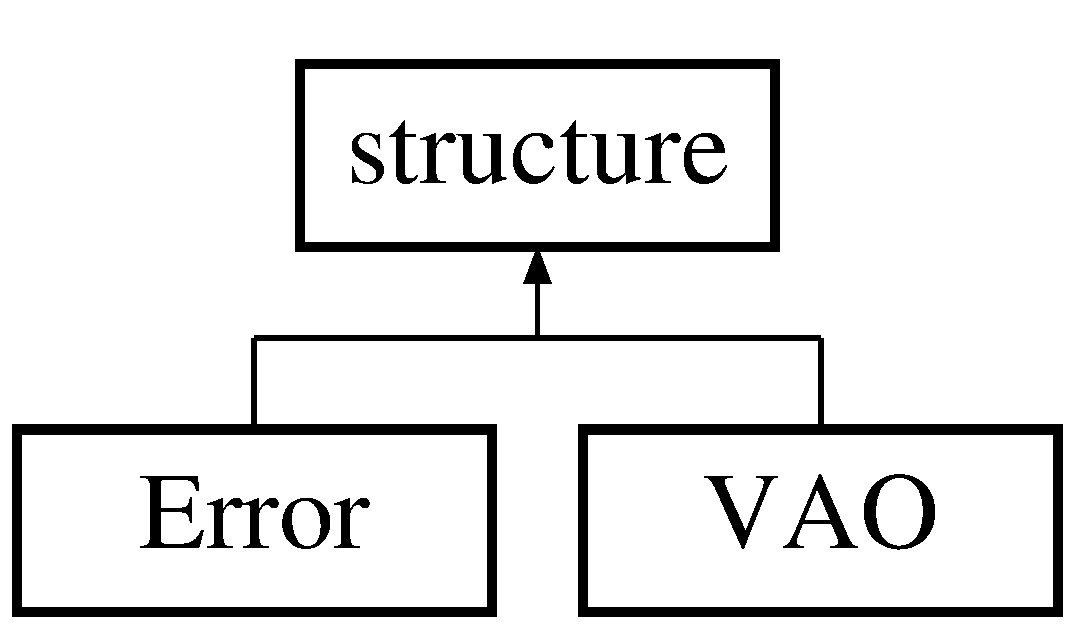
\includegraphics[height=2.000000cm]{classstructure}
\end{center}
\end{figure}


The documentation for this class was generated from the following file\-:\begin{DoxyCompactItemize}
\item 
E\-:/\-G\-R\-A\-B\-L\-A\-U\-R\-G/\-I\-S\-E/\-I\-S\-E-\/\-Demo/\-I\-S\-E-\/\-Demo/V\-A\-O.\-h\end{DoxyCompactItemize}

\hypertarget{class_texture}{\section{Texture Class Reference}
\label{class_texture}\index{Texture@{Texture}}
}


Loads in the texture from a file.  




{\ttfamily \#include $<$Texture.\-h$>$}

\subsection*{Public Member Functions}
\begin{DoxyCompactItemize}
\item 
void \hyperlink{class_texture_aca0c643c48ba3ae98d4effa09eed1737}{load} (std\-::string location)
\begin{DoxyCompactList}\small\item\em Load in texture from the a location. \end{DoxyCompactList}\item 
void \hyperlink{class_texture_a3840dc7429982ffaddeafc8d62345b5d}{bind} ()
\begin{DoxyCompactList}\small\item\em bind the texture \end{DoxyCompactList}\end{DoxyCompactItemize}


\subsection{Detailed Description}
Loads in the texture from a file. 

This class handles loading all the textures and Binding them to open\-G\-L \begin{DoxyReturn}{Returns}
N/\-A 
\end{DoxyReturn}
\begin{DoxyAuthor}{Author}
Umar Badat 
\end{DoxyAuthor}
\begin{DoxyNote}{Note}
Because it was not possible to seperate the sfml \hyperlink{class_texture}{Texture} into a data structure of my own. I could not seperate the functionality from the data so the texture could not be done independantly of the texture object 
\end{DoxyNote}


\subsection{Member Function Documentation}
\hypertarget{class_texture_a3840dc7429982ffaddeafc8d62345b5d}{\index{Texture@{Texture}!bind@{bind}}
\index{bind@{bind}!Texture@{Texture}}
\subsubsection[{bind}]{\setlength{\rightskip}{0pt plus 5cm}void Texture\-::bind (
\begin{DoxyParamCaption}
{}
\end{DoxyParamCaption}
)}}\label{class_texture_a3840dc7429982ffaddeafc8d62345b5d}


bind the texture 

Bind the \hyperlink{class_texture}{Texture} stored in this class to any polygons drawn after it \begin{DoxyNote}{Note}
It might be an idea to find the glu\-Ints so i can manage the memory and reduce a need to pass large objects around. 
\end{DoxyNote}
\hypertarget{class_texture_aca0c643c48ba3ae98d4effa09eed1737}{\index{Texture@{Texture}!load@{load}}
\index{load@{load}!Texture@{Texture}}
\subsubsection[{load}]{\setlength{\rightskip}{0pt plus 5cm}void Texture\-::load (
\begin{DoxyParamCaption}
\item[{std\-::string}]{location}
\end{DoxyParamCaption}
)}}\label{class_texture_aca0c643c48ba3ae98d4effa09eed1737}


Load in texture from the a location. 

Loads in a texture from the given location and stores the texture data within this class. binding is a function from within this class as well


\begin{DoxyParams}{Parameters}
{\em location} & A string to the location of the data \\
\hline
\end{DoxyParams}
\begin{DoxyNote}{Note}
It would have been nice to seperate the data from the function so I could keep components sperated 
\end{DoxyNote}


The documentation for this class was generated from the following files\-:\begin{DoxyCompactItemize}
\item 
E\-:/\-G\-R\-A\-B\-L\-A\-U\-R\-G/\-I\-S\-E/\-I\-S\-E-\/\-Demo/\-I\-S\-E-\/\-Demo/Texture.\-h\item 
E\-:/\-G\-R\-A\-B\-L\-A\-U\-R\-G/\-I\-S\-E/\-I\-S\-E-\/\-Demo/\-I\-S\-E-\/\-Demo/Texture.\-cpp\end{DoxyCompactItemize}

\hypertarget{class_v_a_o}{\section{V\-A\-O Class Reference}
\label{class_v_a_o}\index{V\-A\-O@{V\-A\-O}}
}
Inheritance diagram for V\-A\-O\-:\begin{figure}[H]
\begin{center}
\leavevmode
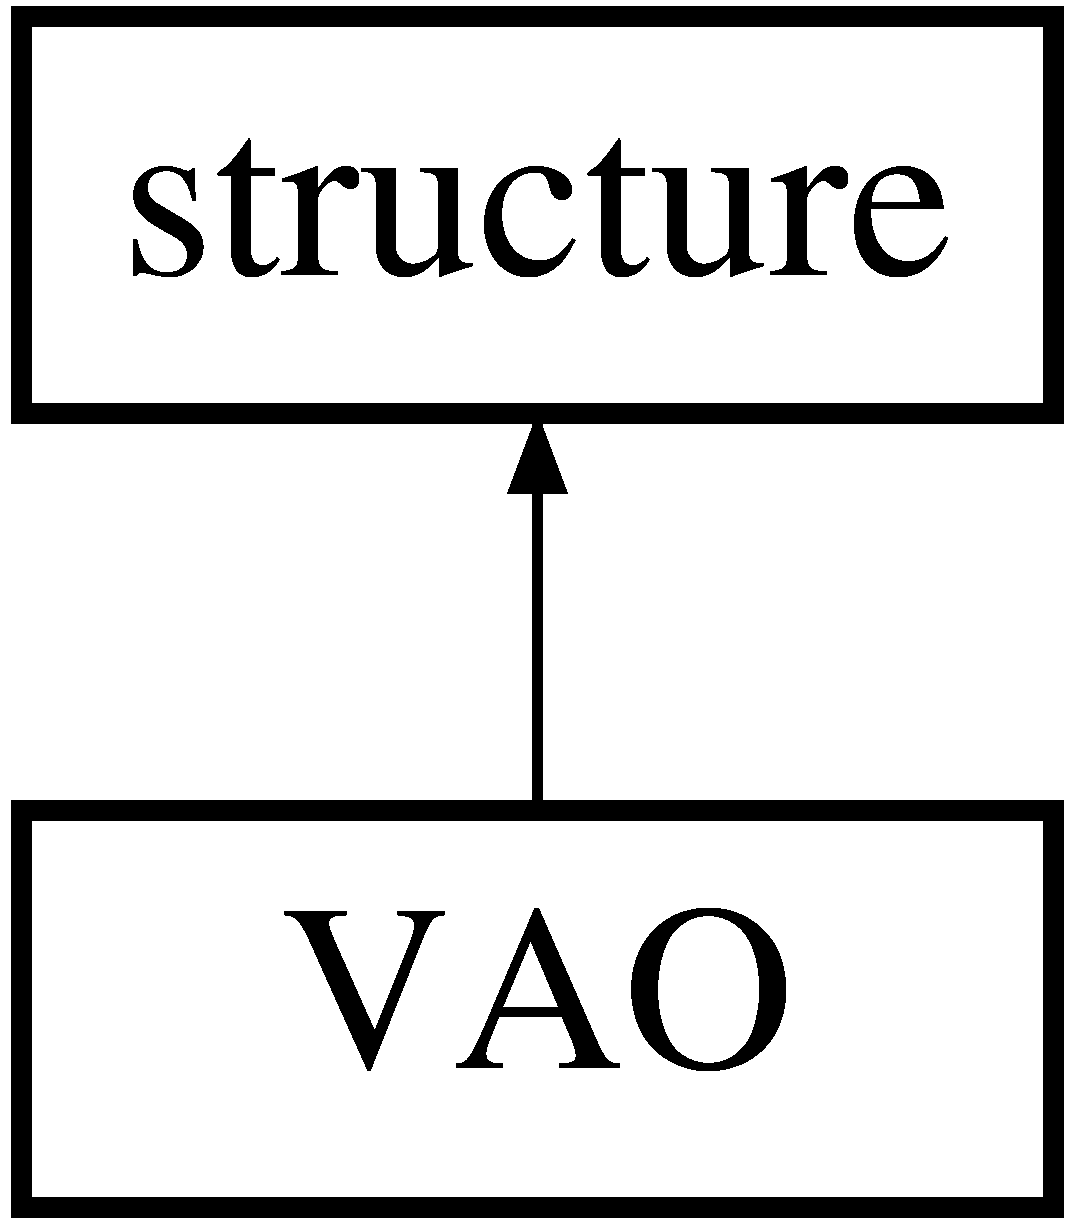
\includegraphics[height=2.000000cm]{class_v_a_o}
\end{center}
\end{figure}
\subsection*{Public Attributes}
\begin{DoxyCompactItemize}
\item 
\hypertarget{class_v_a_o_a4bb703efebc8b659fafb9214df1c00a2}{float $\ast$ {\bfseries vertex\-Array}}\label{class_v_a_o_a4bb703efebc8b659fafb9214df1c00a2}

\item 
\hypertarget{class_v_a_o_a8cac351866d092035d0dd3e1db550443}{float $\ast$ {\bfseries normal\-Array}}\label{class_v_a_o_a8cac351866d092035d0dd3e1db550443}

\item 
\hypertarget{class_v_a_o_a151242cdc48c1f31b1db972e0ed623b3}{float $\ast$ {\bfseries uv\-Array}}\label{class_v_a_o_a151242cdc48c1f31b1db972e0ed623b3}

\item 
\hypertarget{class_v_a_o_a25d570ad1a339b9928f34f920cbae339}{int {\bfseries num\-Verts}}\label{class_v_a_o_a25d570ad1a339b9928f34f920cbae339}

\end{DoxyCompactItemize}


The documentation for this class was generated from the following file\-:\begin{DoxyCompactItemize}
\item 
E\-:/\-G\-R\-A\-B\-L\-A\-U\-R\-G/\-I\-S\-E/\-I\-S\-E-\/\-Demo/\-I\-S\-E-\/\-Demo/V\-A\-O.\-h\end{DoxyCompactItemize}

\hypertarget{struct_vector3}{\section{Vector3 Struct Reference}
\label{struct_vector3}\index{Vector3@{Vector3}}
}


The \hyperlink{struct_vector3}{Vector3} struct.  




{\ttfamily \#include $<$Vector3.\-h$>$}

\subsection*{Public Member Functions}
\begin{DoxyCompactItemize}
\item 
\hypertarget{struct_vector3_a0f49191f7e001e7f7ae1cb49522118b4}{\hyperlink{struct_vector3_a0f49191f7e001e7f7ae1cb49522118b4}{Vector3} ()}\label{struct_vector3_a0f49191f7e001e7f7ae1cb49522118b4}

\begin{DoxyCompactList}\small\item\em Default constuctor for \hyperlink{struct_vector3}{Vector3}. \end{DoxyCompactList}\item 
\hypertarget{struct_vector3_ac599dbf981021aed3af55e48b17a20de}{\hyperlink{struct_vector3_ac599dbf981021aed3af55e48b17a20de}{Vector3} (float new\-X, float new\-Y, float new\-Z)}\label{struct_vector3_ac599dbf981021aed3af55e48b17a20de}

\begin{DoxyCompactList}\small\item\em Constuctor for \hyperlink{struct_vector3}{Vector3} setting up the vectors. \end{DoxyCompactList}\item 
\hyperlink{struct_vector3}{Vector3} \hyperlink{struct_vector3_a15fe643f1a60db32bc90fada912d5886}{operator+} (\hyperlink{struct_vector3}{Vector3} pos)
\begin{DoxyCompactList}\small\item\em \mbox{[}brief description\mbox{]} \end{DoxyCompactList}\item 
\hyperlink{struct_vector3}{Vector3} \hyperlink{struct_vector3_a5652cc75947bccd44a04a353226f3943}{operator-\/} (\hyperlink{struct_vector3}{Vector3} pos)
\begin{DoxyCompactList}\small\item\em \mbox{[}brief description\mbox{]} \end{DoxyCompactList}\item 
\hyperlink{struct_vector3}{Vector3} \hyperlink{struct_vector3_aabd796697d63625e0a6723e0d88f8da7}{operator$\ast$} (\hyperlink{struct_vector3}{Vector3} pos)
\begin{DoxyCompactList}\small\item\em \mbox{[}brief description\mbox{]} \end{DoxyCompactList}\item 
\hyperlink{struct_vector3}{Vector3} \hyperlink{struct_vector3_af9c4cf04f1023d5933416d6c931a54cc}{operator/} (\hyperlink{struct_vector3}{Vector3} pos)
\begin{DoxyCompactList}\small\item\em \mbox{[}brief description\mbox{]} \end{DoxyCompactList}\end{DoxyCompactItemize}
\subsection*{Public Attributes}
\begin{DoxyCompactItemize}
\item 
\hypertarget{struct_vector3_ae3c898eb50be07d39f16964b0328f395}{float {\bfseries m\-\_\-\-X}}\label{struct_vector3_ae3c898eb50be07d39f16964b0328f395}

\item 
\hypertarget{struct_vector3_ac36308f26ba3de04273290a8d430bd3a}{float {\bfseries m\-\_\-\-Y}}\label{struct_vector3_ac36308f26ba3de04273290a8d430bd3a}

\item 
\hypertarget{struct_vector3_aed5814ac3580ece53e3da338346a14ff}{float {\bfseries m\-\_\-\-Z}}\label{struct_vector3_aed5814ac3580ece53e3da338346a14ff}

\end{DoxyCompactItemize}


\subsection{Detailed Description}
The \hyperlink{struct_vector3}{Vector3} struct. 

\begin{DoxyRefDesc}{Bug}
\item[\hyperlink{bug__bug000005}{Bug}]\begin{DoxyNote}{Note}

\end{DoxyNote}
\begin{DoxyAuthor}{Author}
Welsley Gai-\/\-Yeen Lui 
\end{DoxyAuthor}
\begin{DoxyDate}{Date}

\end{DoxyDate}
\end{DoxyRefDesc}


\subsection{Member Function Documentation}
\hypertarget{struct_vector3_aabd796697d63625e0a6723e0d88f8da7}{\index{Vector3@{Vector3}!operator$\ast$@{operator$\ast$}}
\index{operator$\ast$@{operator$\ast$}!Vector3@{Vector3}}
\subsubsection[{operator$\ast$}]{\setlength{\rightskip}{0pt plus 5cm}{\bf Vector3} Vector3\-::operator$\ast$ (
\begin{DoxyParamCaption}
\item[{{\bf Vector3}}]{pos}
\end{DoxyParamCaption}
)\hspace{0.3cm}{\ttfamily [inline]}}}\label{struct_vector3_aabd796697d63625e0a6723e0d88f8da7}


\mbox{[}brief description\mbox{]} 

\mbox{[}long description\mbox{]}


\begin{DoxyParams}{Parameters}
{\em pos} & \mbox{[}description\mbox{]} \\
\hline
{\em pos} & \mbox{[}description\mbox{]} \\
\hline
{\em pos} & \mbox{[}description\mbox{]} \\
\hline
\end{DoxyParams}
\begin{DoxyReturn}{Returns}
\mbox{[}description\mbox{]} 
\end{DoxyReturn}
\hypertarget{struct_vector3_a15fe643f1a60db32bc90fada912d5886}{\index{Vector3@{Vector3}!operator+@{operator+}}
\index{operator+@{operator+}!Vector3@{Vector3}}
\subsubsection[{operator+}]{\setlength{\rightskip}{0pt plus 5cm}{\bf Vector3} Vector3\-::operator+ (
\begin{DoxyParamCaption}
\item[{{\bf Vector3}}]{pos}
\end{DoxyParamCaption}
)\hspace{0.3cm}{\ttfamily [inline]}}}\label{struct_vector3_a15fe643f1a60db32bc90fada912d5886}


\mbox{[}brief description\mbox{]} 

\mbox{[}long description\mbox{]}


\begin{DoxyParams}{Parameters}
{\em pos} & \mbox{[}description\mbox{]} \\
\hline
\end{DoxyParams}
\begin{DoxyReturn}{Returns}
\mbox{[}description\mbox{]} 
\end{DoxyReturn}
\hypertarget{struct_vector3_a5652cc75947bccd44a04a353226f3943}{\index{Vector3@{Vector3}!operator-\/@{operator-\/}}
\index{operator-\/@{operator-\/}!Vector3@{Vector3}}
\subsubsection[{operator-\/}]{\setlength{\rightskip}{0pt plus 5cm}{\bf Vector3} Vector3\-::operator-\/ (
\begin{DoxyParamCaption}
\item[{{\bf Vector3}}]{pos}
\end{DoxyParamCaption}
)\hspace{0.3cm}{\ttfamily [inline]}}}\label{struct_vector3_a5652cc75947bccd44a04a353226f3943}


\mbox{[}brief description\mbox{]} 

\mbox{[}long description\mbox{]}


\begin{DoxyParams}{Parameters}
{\em pos} & \mbox{[}description\mbox{]} \\
\hline
\end{DoxyParams}
\begin{DoxyReturn}{Returns}
\mbox{[}description\mbox{]} 
\end{DoxyReturn}
\hypertarget{struct_vector3_af9c4cf04f1023d5933416d6c931a54cc}{\index{Vector3@{Vector3}!operator/@{operator/}}
\index{operator/@{operator/}!Vector3@{Vector3}}
\subsubsection[{operator/}]{\setlength{\rightskip}{0pt plus 5cm}{\bf Vector3} Vector3\-::operator/ (
\begin{DoxyParamCaption}
\item[{{\bf Vector3}}]{pos}
\end{DoxyParamCaption}
)\hspace{0.3cm}{\ttfamily [inline]}}}\label{struct_vector3_af9c4cf04f1023d5933416d6c931a54cc}


\mbox{[}brief description\mbox{]} 

\mbox{[}long description\mbox{]}


\begin{DoxyParams}{Parameters}
{\em pos} & \mbox{[}description\mbox{]} \\
\hline
\end{DoxyParams}
\begin{DoxyReturn}{Returns}
\mbox{[}description\mbox{]} 
\end{DoxyReturn}


The documentation for this struct was generated from the following file\-:\begin{DoxyCompactItemize}
\item 
E\-:/\-G\-R\-A\-B\-L\-A\-U\-R\-G/\-I\-S\-E/\-I\-S\-E-\/\-Demo/\-I\-S\-E-\/\-Demo/Vector3.\-h\end{DoxyCompactItemize}

\hypertarget{class_window}{\section{Window Class Reference}
\label{class_window}\index{Window@{Window}}
}
\subsection*{Public Member Functions}
\begin{DoxyCompactItemize}
\item 
\hyperlink{class_window_a4a680ada9e0fea7c45c8c84614cb5699}{Window} (\hyperlink{class_s_f_m_l___facade}{S\-F\-M\-L\-\_\-\-Facade} window)
\begin{DoxyCompactList}\small\item\em copy a window in so both use the same address \end{DoxyCompactList}\item 
void \hyperlink{class_window_ac10f45b63d94348594f65398c0583151}{create} (int width, int height, std\-::string name)
\begin{DoxyCompactList}\small\item\em create a window \end{DoxyCompactList}\item 
void \hyperlink{class_window_a574ee2df1903f21e80b2e1c3ad487339}{set\-Width\-Height} (int width, int height)
\begin{DoxyCompactList}\small\item\em set this window's width and height \end{DoxyCompactList}\item 
void \hyperlink{class_window_a1f38c584ac5fb56dd4de62f56d8e62e3}{set\-Width} (int width)
\begin{DoxyCompactList}\small\item\em set this window's width \end{DoxyCompactList}\item 
void \hyperlink{class_window_af84228b0e73053ce7632bef29047b57b}{set\-Height} (int height)
\begin{DoxyCompactList}\small\item\em set this window's height \end{DoxyCompactList}\item 
void \hyperlink{class_window_ab10e764f00af15dab354b9693db252fe}{set\-Title} (std\-::string name)
\begin{DoxyCompactList}\small\item\em set this window's title \end{DoxyCompactList}\item 
void \hyperlink{class_window_a20e45797c9462dba56ae532fe76cb815}{active} ()
\begin{DoxyCompactList}\small\item\em set this window to the active opengl context \end{DoxyCompactList}\item 
void \hyperlink{class_window_afadfafa5a0b9472554759004aafb327e}{display} ()
\begin{DoxyCompactList}\small\item\em swap buffers \end{DoxyCompactList}\item 
int \hyperlink{class_window_a2d459fe21a48b6a41834a32a6c84fe2e}{get\-Width} ()
\begin{DoxyCompactList}\small\item\em get width \end{DoxyCompactList}\item 
int \hyperlink{class_window_a02acaaf02d8b63d4bd74d99482fe3a78}{get\-Height} ()
\begin{DoxyCompactList}\small\item\em ge height \end{DoxyCompactList}\item 
void \hyperlink{class_window_aeb09abe99d95c2a0e18b376a69ff1829}{enable\-Depth} ()
\begin{DoxyCompactList}\small\item\em enable depth items \end{DoxyCompactList}\item 
void \hyperlink{class_window_aef2dd56a6369e2833e8d28b1c136a92e}{disable\-Depth} ()
\begin{DoxyCompactList}\small\item\em Disable depth items. \end{DoxyCompactList}\item 
void \hyperlink{class_window_a0d3072ad7bb6198c4a8f8b2eee9cb65a}{enable\-Lighting} ()
\begin{DoxyCompactList}\small\item\em enable light \end{DoxyCompactList}\item 
void \hyperlink{class_window_a02569a6c097115bf19dab36eaa5887e0}{disable\-Lighting} ()
\begin{DoxyCompactList}\small\item\em disable lights \end{DoxyCompactList}\item 
void \hyperlink{class_window_ae802af8f8026e3cf48079b83a2fab65d}{colour\-Depth} ()
\begin{DoxyCompactList}\small\item\em set color and depth automatically \end{DoxyCompactList}\item 
void \hyperlink{class_window_a02533f2cb7bbb254b5603173dcb48985}{set\-Colour} (float R, float G, float B)
\begin{DoxyCompactList}\small\item\em set the clear colour \end{DoxyCompactList}\item 
void \hyperlink{class_window_adb9181c38ed81867aeca95fa1fa6b3f7}{set\-Depth} (float Depth)
\begin{DoxyCompactList}\small\item\em set depth \end{DoxyCompactList}\item 
sf\-::\-Window $\ast$ \hyperlink{class_window_a1f00d7696a8ef63e34313e5a5a1224b7}{get\-Event} ()
\begin{DoxyCompactList}\small\item\em Get events function. \end{DoxyCompactList}\item 
\hypertarget{class_window_a59515fc5a56e86d5a46d771595daac55}{void {\bfseries update} ()}\label{class_window_a59515fc5a56e86d5a46d771595daac55}

\item 
void \hyperlink{class_window_aeab5e948ff730b4d7fe503104c52f79c}{set\-Window\-Pos} (int x, int y)
\begin{DoxyCompactList}\small\item\em set window position \end{DoxyCompactList}\item 
void \hyperlink{class_window_aded83fb2975d2c14e7892427dd9bc02e}{get\-Window\-Pos} (int \&x, int \&y)
\begin{DoxyCompactList}\small\item\em get window position \end{DoxyCompactList}\end{DoxyCompactItemize}


\subsection{Constructor \& Destructor Documentation}
\hypertarget{class_window_a4a680ada9e0fea7c45c8c84614cb5699}{\index{Window@{Window}!Window@{Window}}
\index{Window@{Window}!Window@{Window}}
\subsubsection[{Window}]{\setlength{\rightskip}{0pt plus 5cm}Window\-::\-Window (
\begin{DoxyParamCaption}
\item[{{\bf S\-F\-M\-L\-\_\-\-Facade}}]{window}
\end{DoxyParamCaption}
)}}\label{class_window_a4a680ada9e0fea7c45c8c84614cb5699}


copy a window in so both use the same address 

this functio was intended for seperating the input from the render engine while still having access to the events


\begin{DoxyParams}{Parameters}
{\em window} & \hyperlink{class_s_f_m_l___facade}{S\-F\-M\-L\-\_\-\-Facade} window \\
\hline
\end{DoxyParams}
\begin{DoxyRefDesc}{Deprecated}
\item[\hyperlink{deprecated__deprecated000002}{Deprecated}]This function is no longer used, there are better ways to get the key inputs from the user \end{DoxyRefDesc}


\subsection{Member Function Documentation}
\hypertarget{class_window_a20e45797c9462dba56ae532fe76cb815}{\index{Window@{Window}!active@{active}}
\index{active@{active}!Window@{Window}}
\subsubsection[{active}]{\setlength{\rightskip}{0pt plus 5cm}void Window\-::active (
\begin{DoxyParamCaption}
{}
\end{DoxyParamCaption}
)}}\label{class_window_a20e45797c9462dba56ae532fe76cb815}


set this window to the active opengl context 

This window is now going to have all opengl calls applied to it \hypertarget{class_window_ae802af8f8026e3cf48079b83a2fab65d}{\index{Window@{Window}!colour\-Depth@{colour\-Depth}}
\index{colour\-Depth@{colour\-Depth}!Window@{Window}}
\subsubsection[{colour\-Depth}]{\setlength{\rightskip}{0pt plus 5cm}void Window\-::colour\-Depth (
\begin{DoxyParamCaption}
{}
\end{DoxyParamCaption}
)}}\label{class_window_ae802af8f8026e3cf48079b83a2fab65d}


set color and depth automatically 

\mbox{[}long description\mbox{]} \hypertarget{class_window_ac10f45b63d94348594f65398c0583151}{\index{Window@{Window}!create@{create}}
\index{create@{create}!Window@{Window}}
\subsubsection[{create}]{\setlength{\rightskip}{0pt plus 5cm}void Window\-::create (
\begin{DoxyParamCaption}
\item[{int}]{width, }
\item[{int}]{height, }
\item[{std\-::string}]{name}
\end{DoxyParamCaption}
)}}\label{class_window_ac10f45b63d94348594f65398c0583151}


create a window 

create a window with a name width and heigh specified upon creation


\begin{DoxyParams}{Parameters}
{\em width} & int \\
\hline
{\em height} & int \\
\hline
{\em name} & string \\
\hline
\end{DoxyParams}
\hypertarget{class_window_aef2dd56a6369e2833e8d28b1c136a92e}{\index{Window@{Window}!disable\-Depth@{disable\-Depth}}
\index{disable\-Depth@{disable\-Depth}!Window@{Window}}
\subsubsection[{disable\-Depth}]{\setlength{\rightskip}{0pt plus 5cm}void Window\-::disable\-Depth (
\begin{DoxyParamCaption}
{}
\end{DoxyParamCaption}
)}}\label{class_window_aef2dd56a6369e2833e8d28b1c136a92e}


Disable depth items. 

Disable depth test and depth mask \hypertarget{class_window_a02569a6c097115bf19dab36eaa5887e0}{\index{Window@{Window}!disable\-Lighting@{disable\-Lighting}}
\index{disable\-Lighting@{disable\-Lighting}!Window@{Window}}
\subsubsection[{disable\-Lighting}]{\setlength{\rightskip}{0pt plus 5cm}void Window\-::disable\-Lighting (
\begin{DoxyParamCaption}
{}
\end{DoxyParamCaption}
)}}\label{class_window_a02569a6c097115bf19dab36eaa5887e0}


disable lights 

disable the lights in opengl \hypertarget{class_window_afadfafa5a0b9472554759004aafb327e}{\index{Window@{Window}!display@{display}}
\index{display@{display}!Window@{Window}}
\subsubsection[{display}]{\setlength{\rightskip}{0pt plus 5cm}void Window\-::display (
\begin{DoxyParamCaption}
{}
\end{DoxyParamCaption}
)}}\label{class_window_afadfafa5a0b9472554759004aafb327e}


swap buffers 

display all the open\-G\-L calls that have been called \hypertarget{class_window_aeb09abe99d95c2a0e18b376a69ff1829}{\index{Window@{Window}!enable\-Depth@{enable\-Depth}}
\index{enable\-Depth@{enable\-Depth}!Window@{Window}}
\subsubsection[{enable\-Depth}]{\setlength{\rightskip}{0pt plus 5cm}void Window\-::enable\-Depth (
\begin{DoxyParamCaption}
{}
\end{DoxyParamCaption}
)}}\label{class_window_aeb09abe99d95c2a0e18b376a69ff1829}


enable depth items 

Enable depths test and depth mask \hypertarget{class_window_a0d3072ad7bb6198c4a8f8b2eee9cb65a}{\index{Window@{Window}!enable\-Lighting@{enable\-Lighting}}
\index{enable\-Lighting@{enable\-Lighting}!Window@{Window}}
\subsubsection[{enable\-Lighting}]{\setlength{\rightskip}{0pt plus 5cm}void Window\-::enable\-Lighting (
\begin{DoxyParamCaption}
{}
\end{DoxyParamCaption}
)}}\label{class_window_a0d3072ad7bb6198c4a8f8b2eee9cb65a}


enable light 

enable the opengl lights \begin{DoxyRefDesc}{Bug}
\item[\hyperlink{bug__bug000006}{Bug}]the functionality of this has not been implemented yet please don't use it unless you can call light \end{DoxyRefDesc}
\hypertarget{class_window_a1f00d7696a8ef63e34313e5a5a1224b7}{\index{Window@{Window}!get\-Event@{get\-Event}}
\index{get\-Event@{get\-Event}!Window@{Window}}
\subsubsection[{get\-Event}]{\setlength{\rightskip}{0pt plus 5cm}sf\-::\-Window$\ast$ Window\-::get\-Event (
\begin{DoxyParamCaption}
{}
\end{DoxyParamCaption}
)\hspace{0.3cm}{\ttfamily [inline]}}}\label{class_window_a1f00d7696a8ef63e34313e5a5a1224b7}


Get events function. 

This function was used to get to the window so you can poll it \begin{DoxyReturn}{Returns}
sf\-::\-Event 
\end{DoxyReturn}
\begin{DoxyRefDesc}{Deprecated}
\item[\hyperlink{deprecated__deprecated000003}{Deprecated}]This function is no longer used it has been replaced by a better engine \end{DoxyRefDesc}
\hypertarget{class_window_a02acaaf02d8b63d4bd74d99482fe3a78}{\index{Window@{Window}!get\-Height@{get\-Height}}
\index{get\-Height@{get\-Height}!Window@{Window}}
\subsubsection[{get\-Height}]{\setlength{\rightskip}{0pt plus 5cm}int Window\-::get\-Height (
\begin{DoxyParamCaption}
{}
\end{DoxyParamCaption}
)}}\label{class_window_a02acaaf02d8b63d4bd74d99482fe3a78}


ge height 

get th height of the window \begin{DoxyReturn}{Returns}
int height 
\end{DoxyReturn}
\hypertarget{class_window_a2d459fe21a48b6a41834a32a6c84fe2e}{\index{Window@{Window}!get\-Width@{get\-Width}}
\index{get\-Width@{get\-Width}!Window@{Window}}
\subsubsection[{get\-Width}]{\setlength{\rightskip}{0pt plus 5cm}int Window\-::get\-Width (
\begin{DoxyParamCaption}
{}
\end{DoxyParamCaption}
)}}\label{class_window_a2d459fe21a48b6a41834a32a6c84fe2e}


get width 

get the width of the window \begin{DoxyReturn}{Returns}
int width 
\end{DoxyReturn}
\hypertarget{class_window_aded83fb2975d2c14e7892427dd9bc02e}{\index{Window@{Window}!get\-Window\-Pos@{get\-Window\-Pos}}
\index{get\-Window\-Pos@{get\-Window\-Pos}!Window@{Window}}
\subsubsection[{get\-Window\-Pos}]{\setlength{\rightskip}{0pt plus 5cm}void Window\-::get\-Window\-Pos (
\begin{DoxyParamCaption}
\item[{int \&}]{x, }
\item[{int \&}]{y}
\end{DoxyParamCaption}
)}}\label{class_window_aded83fb2975d2c14e7892427dd9bc02e}


get window position 

get window position on screenn


\begin{DoxyParams}{Parameters}
{\em x} & int pass in address the value is then assigned to it \\
\hline
{\em y} & int pass in address the value is then assigned to it \\
\hline
\end{DoxyParams}
\hypertarget{class_window_a02533f2cb7bbb254b5603173dcb48985}{\index{Window@{Window}!set\-Colour@{set\-Colour}}
\index{set\-Colour@{set\-Colour}!Window@{Window}}
\subsubsection[{set\-Colour}]{\setlength{\rightskip}{0pt plus 5cm}void Window\-::set\-Colour (
\begin{DoxyParamCaption}
\item[{float}]{R, }
\item[{float}]{G, }
\item[{float}]{B}
\end{DoxyParamCaption}
)}}\label{class_window_a02533f2cb7bbb254b5603173dcb48985}


set the clear colour 


\begin{DoxyParams}{Parameters}
{\em R} & Red \\
\hline
{\em G} & Green \\
\hline
{\em B} & Blue \\
\hline
\end{DoxyParams}
\hypertarget{class_window_adb9181c38ed81867aeca95fa1fa6b3f7}{\index{Window@{Window}!set\-Depth@{set\-Depth}}
\index{set\-Depth@{set\-Depth}!Window@{Window}}
\subsubsection[{set\-Depth}]{\setlength{\rightskip}{0pt plus 5cm}void Window\-::set\-Depth (
\begin{DoxyParamCaption}
\item[{float}]{Depth}
\end{DoxyParamCaption}
)}}\label{class_window_adb9181c38ed81867aeca95fa1fa6b3f7}


set depth 


\begin{DoxyParams}{Parameters}
{\em Depth} & depth \\
\hline
\end{DoxyParams}
\hypertarget{class_window_af84228b0e73053ce7632bef29047b57b}{\index{Window@{Window}!set\-Height@{set\-Height}}
\index{set\-Height@{set\-Height}!Window@{Window}}
\subsubsection[{set\-Height}]{\setlength{\rightskip}{0pt plus 5cm}void Window\-::set\-Height (
\begin{DoxyParamCaption}
\item[{int}]{height}
\end{DoxyParamCaption}
)}}\label{class_window_af84228b0e73053ce7632bef29047b57b}


set this window's height 

the height of this window is set here


\begin{DoxyParams}{Parameters}
{\em height} & int \\
\hline
\end{DoxyParams}
\hypertarget{class_window_ab10e764f00af15dab354b9693db252fe}{\index{Window@{Window}!set\-Title@{set\-Title}}
\index{set\-Title@{set\-Title}!Window@{Window}}
\subsubsection[{set\-Title}]{\setlength{\rightskip}{0pt plus 5cm}void Window\-::set\-Title (
\begin{DoxyParamCaption}
\item[{std\-::string}]{name}
\end{DoxyParamCaption}
)}}\label{class_window_ab10e764f00af15dab354b9693db252fe}


set this window's title 

the title of this window is set here


\begin{DoxyParams}{Parameters}
{\em name} & string \\
\hline
\end{DoxyParams}
\hypertarget{class_window_a1f38c584ac5fb56dd4de62f56d8e62e3}{\index{Window@{Window}!set\-Width@{set\-Width}}
\index{set\-Width@{set\-Width}!Window@{Window}}
\subsubsection[{set\-Width}]{\setlength{\rightskip}{0pt plus 5cm}void Window\-::set\-Width (
\begin{DoxyParamCaption}
\item[{int}]{width}
\end{DoxyParamCaption}
)}}\label{class_window_a1f38c584ac5fb56dd4de62f56d8e62e3}


set this window's width 

the width of this window is set here


\begin{DoxyParams}{Parameters}
{\em width} & int \\
\hline
\end{DoxyParams}
\hypertarget{class_window_a574ee2df1903f21e80b2e1c3ad487339}{\index{Window@{Window}!set\-Width\-Height@{set\-Width\-Height}}
\index{set\-Width\-Height@{set\-Width\-Height}!Window@{Window}}
\subsubsection[{set\-Width\-Height}]{\setlength{\rightskip}{0pt plus 5cm}void Window\-::set\-Width\-Height (
\begin{DoxyParamCaption}
\item[{int}]{width, }
\item[{int}]{height}
\end{DoxyParamCaption}
)}}\label{class_window_a574ee2df1903f21e80b2e1c3ad487339}


set this window's width and height 

the width and height of this window is set by two numbers


\begin{DoxyParams}{Parameters}
{\em width} & int \\
\hline
{\em height} & int \\
\hline
\end{DoxyParams}
\hypertarget{class_window_aeab5e948ff730b4d7fe503104c52f79c}{\index{Window@{Window}!set\-Window\-Pos@{set\-Window\-Pos}}
\index{set\-Window\-Pos@{set\-Window\-Pos}!Window@{Window}}
\subsubsection[{set\-Window\-Pos}]{\setlength{\rightskip}{0pt plus 5cm}void Window\-::set\-Window\-Pos (
\begin{DoxyParamCaption}
\item[{int}]{x, }
\item[{int}]{y}
\end{DoxyParamCaption}
)}}\label{class_window_aeab5e948ff730b4d7fe503104c52f79c}


set window position 

set the window positio on the screen


\begin{DoxyParams}{Parameters}
{\em x} & int x position on screen \\
\hline
{\em y} & int y position on screen \\
\hline
\end{DoxyParams}


The documentation for this class was generated from the following files\-:\begin{DoxyCompactItemize}
\item 
E\-:/\-G\-R\-A\-B\-L\-A\-U\-R\-G/\-I\-S\-E/\-I\-S\-E-\/\-Demo/\-I\-S\-E-\/\-Demo/Window.\-h\item 
E\-:/\-G\-R\-A\-B\-L\-A\-U\-R\-G/\-I\-S\-E/\-I\-S\-E-\/\-Demo/\-I\-S\-E-\/\-Demo/Window.\-cpp\end{DoxyCompactItemize}

%--- End generated contents ---

% Index
\newpage
\phantomsection
\addcontentsline{toc}{chapter}{Index}
\printindex

\end{document}
